\documentclass{book}

%
% Use Times font
%
\usepackage[T1]{fontenc}
\usepackage{textcomp}
\usepackage{times}
%\usepackage{mathtime}
\usepackage[scaled=0.8]{luximono}
\usepackage{listings}
\usepackage{fancyhdr}
\usepackage{fancyvrb}
\usepackage{makeidx}
\usepackage{proof}
\usepackage{graphicx}
\usepackage{setspace}
%\doublespacing

%%%%%%%%%%%%%%%%%%%%%%%%%%%%%%%%%%%%%%%%%%%%%%%%%%%%%%%%%%%%%%%%%%%%%%%%%
% METAPRL DEFINITIONS
%%%%%%%%%%%%%%%%%%%%%%%%%%%%%%%%%%%%%%%%%%%%%%%%%%%%%%%%%%%%%%%%%%%%%%%%%

%
% Make sure \|,\< and \> always produce an appropriate symbol
%
\def\|{\ifmmode\mid\else$\mid$\fi}
\def\lt{\ifmmode<\else\texttt{<}\fi}
\def\gt{\ifmmode>\else\texttt{>}\fi}
\def\makehat{\ifmmode\hat{\ }\else\^{}\fi}

%
% Sectioning commands
%
\newcommand\theory[1]{\chapter{#1}}
\newcommand\module[1]{\section{#1}}
\newcommand\labelmodule[2]{\section{#2 module}
  \hypertarget{hypmodule:#1}{}
  \label{module:#1}}
\newcommand\modsection[1]{\subsection{#1}}
\newcommand\modsubsection[1]{\subsubsection{#1}}
\newcommand\labelchapter[2]{\chapter{#2}%
  %\hypertarget{hypsection:#1}{}
  \label{chapter:#1}%
  \label{section:#1}%
  %HEVEA\cutname{#1.html}
  \setcounter{doexercise}{0}}
\newcommand\labelsection[2]{\section{#2}%
  %\hypertarget{hypsection:#1}{}%
  \label{section:#1}}
\newcommand\labelsubsection[2]{\subsection{#2}%
  %\hypertarget{hypsection:#1}{}
  \label{section:#1}}
\newcommand\labelsubsubsection[2]{\subsubsection{#2}%
  %\hypertarget{hypsection:#1}{}
  \label{section:#1}}

\newcommand\hreflabelmodule[2]{\hyperlink{hypmodule:#1}{{\tt #2}}}
\newcommand\reflabelmodule[1]{\ref{module:#1}}

\newcommand\hreflabelchapter[2]{\hyperlink{hypsection:#1}{{\tt #2}}}
\newcommand\reflabelchapter[1]{\ref{section:#1}}

\newcommand\hreflabelsection[2]{\hyperlink{hypsection:#1}{{\tt #2}}}
\newcommand\reflabelsection[1]{\ref{section:#1}}

\newcommand\hreflabelsubsection[2]{\hyperlink{hypsection:#1}{{\tt #2}}}
\newcommand\reflabelsubsection[1]{\ref{section:#1}}

\newcommand\hreflabelsubsubsection[2]{\hyperlink{hypsection:#1}{{\tt #2}}}
\newcommand\reflabelsubsubsection[1]{\ref{section:#1}}

\newcommand\parents{\thysection{Parents}}
%\newcommand\terms{\thysection{Terms}}
\newcommand\resources{\thysection{Resources}}
\newcommand\tactics{\thysection{Tactics}}
\newcommand\tacticals{\thysection{Tacticals}}
\newcommand\rules{\thysection{Rules}}
\newcommand\rewrites{\thysection{Rewrites}}
\newcommand\conversions{\thysection{Conversions}}
\newcommand\conversionals{\thysection{Conversionals}}
\newcommand\convs{\thysection{Conversions}}

%
% Hyperlinks
%
\newcommand\labeltarget[2]{%
  \label{target:#1}
  \hypertarget{hyptarget:#1}{{\tt #2}}\index{Targets!#1@{\it #2}}}

\newcommand\labelterm[2]{%
  \label{term:#1}
  \hypertarget{hypterm:#1}{{\tt #2}}\index{Terms!#1@{\it #2}}}
\newcommand\labelresource[2]{%
  \label{resource:#1}
  \hypertarget{hypresource:#1}{{\tt #2}}\index{Resources!#1@{\it #2}}}
\newcommand\labelrewrite[2]{%
  \label{rewrite:#1}
  \hypertarget{hyprewrite:#1}{{\tt #2}}\index{Rewrites!#1@{\it #2}}}
\newcommand\labeltactic[2]{%
  \label{tactic:#1}
  \hypertarget{hyptactic:#1}{{\tt #2}}\index{Tactics!#1@{\it #2}}}
\newcommand\labelconv[2]{%
  \label{conv:#1}
  \hypertarget{hypconv:#1}{{\tt #2}}\index{Conversions!#1@{\it #2}}}
\newcommand\labelrule[2]{%
  \label{rule:#1}
  \hypertarget{hyprule:#1}{{\tt #2}}\index{Rules!#1@{\it #2}}}

\newcommand\hreflabeltarget[2]{\hyperlink{hyptarget:#1}{{\tt #2}}}
\newcommand\hreflabelterm[2]{\hyperlink{hypterm:#1}{{\tt #2}}}
\newcommand\hreflabelresource[2]{\hyperlink{hypresource:#1}{{\tt #2}}}
\newcommand\hreflabelrewrite[2]{\hyperlink{hyprewrite:#1}{{\tt #2}}}
\newcommand\hreflabeltactic[2]{\hyperlink{hyptactic:#1}{{\tt #2}}}
\newcommand\hreflabelconv[2]{\hyperlink{hypconv:#1}{{\tt #2}}}
\newcommand\hreflabelrule[2]{\hyperlink{hyprule:#1}{{\tt #2}}}

\newcommand\reftarget[1]{\pageref{target:#1}}
\newcommand\refterm[1]{\pageref{term:#1}}
\newcommand\refresource[1]{\pageref{resource:#1}}
\newcommand\refrewrite[1]{\pageref{rewrite:#1}}
\newcommand\reftactic[1]{\pageref{tactic:#1}}
\newcommand\refconv[1]{\pageref{conv:#1}}
\newcommand\refrule[1]{\pageref{rule:#1}}

\newcommand\reflabeltarget[1]{\pageref{target:#1}}
\newcommand\reflabelterm[1]{\pageref{term:#1}}
\newcommand\reflabelresource[1]{\pageref{resource:#1}}
\newcommand\reflabelrewrite[1]{\pageref{rewrite:#1}}
\newcommand\reflabeltactic[1]{\pageref{tactic:#1}}
\newcommand\reflabelconv[1]{\pageref{conv:#1}}
\newcommand\reflabelrule[1]{\pageref{rule:#1}}

\newcommand\labelfigure[1]{\label{figure:#1}}
\newcommand\reffigure[1]{\ref{figure:#1}}

%
% Macros for the OCaml book.
%
\newcommand\note[1]{}
\newcommand\misspelled[1]{#1}

\newcommand\OCaml{OCaml}

%
% Basic macros
%
\newcommand\mr[1]{\textrm{#1}}
\newcommand\ms[1]{\textit{#1}}
\newcommand\mt[1]{\texttt{#1}}
\newcommand\mb[1]{\textbf{#1}}
\newcommand\vbar{\mathrel{|}}
\newcommand\ttemph[1]{\texttt{\emph{#1}}}
\newcommand\nt[1]{\ms{\rmfamily #1}}

\newcommand\subtype{\mathrel{\hbox{<:}}}

\newcommand\pipe{|}

%
% An indented paragraph.
%
% \renewenvironment{indent}
%     {\begin{center}
%      \begin{minipage}{\innerwidth}}
%     {\end{minipage}
%      \end{center}}

%
% Comments
%
\newif\ifcomment
\commenttrue
\newdimen\columnwidth
\setlength\columnwidth{\textwidth}
\newdimen\commentwidth
\setlength{\commentwidth}{\columnwidth}
\newcommand\comment[1]{%
  \ifcomment
    \begin{center}
      \advance\commentwidth by -0.5in
      \fbox{\begin{minipage}{\commentwidth}
            \sf #1
            \end{minipage}}
    \end{center}
  \fi}
\newcommand\nocomment[1]{}

%
% Marginal comments.
%
% Commenting symbol
%
\newcommand\commentsym{%
\begin{picture}(9, 7)
\put(4, 3.5){\circle{6}}
\put(1, 3.5){\line(1,0){6}}
\end{picture}}
%
% Comment in the margin.
%
\newcommand\mcomment[1]{%
   \ifcomment
      \commentsym\marginpar{\commentsym \em #1}
   \fi}

%
% Comment in a footnote
%
\newcommand\fcomment[1]{%
   \ifcomment
      \footnote{\comment{#1}}
   \fi}

%%%%%%%%%%%%%%%%%%%%%%%%%%%%%%%%%%%%%%%%%%%%%%%%%%%%%%%%%%%%%%%%%%%%%%%%
% Display
%

%
% Use verbatim environments for the toploop.
%
\DefineVerbatimEnvironment{topoutput}{BVerbatim}{fontshape=it}
\DefineVerbatimEnvironment{toperror}{BVerbatim}{fontshape=it}

%%%%%%%%%%%%%%%%%%%%%%%%%%%%%%%%%%%%%%%%%%%%%%%%%%%%%%%%%%%%%%%%%%%%%%%%
% Exercise section.
%
% \answers       : set if we are printing the answers
%
\newif\ifanswers
\answersfalse

\newtheorem{doexercise}{Exercise}
\newenvironment{exercise}[1]
{%
\begin{doexercise}
   \label{exercise:#1}
   \ifanswers
   \else
      \rm
   \fi
}
{\end{doexercise}}
\renewcommand\thedoexercise{\thechapter.\arabic{doexercise}}

%
% The box is just for comments.  If we don't want the answers,
% put them into a box and forget about it.
%
\newenvironment{answer}
{\rm}
{}

\newcommand\exercises{%
\section{Exercises}
\setcounter{doexercise}{0}}

\newcommand\answers{%
\answerstrue
\chapter{Answers to exercises}
\renewcommand\thedoexercise{\thesection.\arabic{doexercise}}}

%%%%%%%%%%%%%%%%%%%%%%%%%%%%%%%%%%%%%%%%%%%%%%%%%%%%%%%%%%%%%%%%%%%%%%%%
% Figures
%
\newcommand\refchapter[1]{\ref{chapter:#1}}
\newcommand\refsection[1]{\ref{section:#1}}

\newcommand\makefigure[3]{%
   \begin{figure}[#2]
   #3
   \label{figure:#1}
   \end{figure}}

%
% XXX: Hypertext target
%
\newcommand\xline[1]{#1}
\newcommand\target[2]{#2}

% -*-
% Local Variables:
% Mode: LaTeX
% fill-column: 100
% TeX-master: "paper"
% TeX-command-default: "LaTeX/dvips Interactive"
% End:
% -*-

%
% Generic environment for wrapping code blocks
%
\newenvironment{lstblock}{}{}

%
% OCaml listings.
%
\lstdefinestyle{ocaml}{%
    language=[Objective]Caml,
    basicstyle=\ttfamily,
    keywordstyle=\bfseries\ttfamily,
    breaklines=true,
    mathescape=true,
    alsoletter={'},
    columns=flexible,
    morekeywords={raise,initializer}}
\newcommand\ocamlenv{%
   \setstretch{1}    % Single spacing
   \lstset{%
        style=ocaml,
        showstringspaces=false,
        resetmargins=false,
        columns=[c]fixed,
        keepspaces=true}}
\newcommand\ocamlboxenv{%
    \ocamlenv
    \lstset{%
        boxpos=t,
        aboveskip=8pt,
        belowskip=8pt,
        xleftmargin=4em,
        escapechar=@}}
\newcommand\ocamlbox{%
    \footnotesize
    \ocamlboxenv}

%
% Define the default as OCaml, so we can use lstinline.
% This environment is used only for \hbox{\lstinline/.../},
% keywords should not be bold.
%
\lstset{%
    style=ocaml,
    showstringspaces=false,
    columns=[c]fixed,
    keepspaces=true,
    keywordstyle=\ttfamily}

%
% OLD STYLE: the text is not indented, and no margin
% This is still appropriate to use within lists.
%
\lstnewenvironment{ocamllisting}
   {%XHEVEA\setenvclass{lstlisting}{ocamllisting}
    \footnotesize
    \ocamlenv
    \lstset{%
        boxpos=t,
        aboveskip=0pt,
        belowskip=0pt}}
   {}

\lstnewenvironment{ocamllistinge}
   {%XHEVEA\setenvclass{lstlisting}{ocamllisting}
    %\footnotesize
    \ocamlenv
    \lstset{%
        boxpos=t,
        aboveskip=0pt,
        belowskip=0pt}}
   {}

\lstnewenvironment{ocamllistingx}
   {%XHEVEA\setenvclass{lstlisting}{ocamllisting}
    \footnotesize
    \ocamlenv
    \lstset{%
        boxpos=t,
        aboveskip=0pt,
        belowskip=0pt,
        escapechar=@}}
   {}

\lstnewenvironment{ocamllistingy}
   {%XHEVEA\setenvclass{lstlisting}{ocamllisting}
    \footnotesize
    \ocamlenv
    \lstset{%
        boxpos=t,
        aboveskip=0pt,
        belowskip=0pt,
        escapechar=@}}
   {}

%
% NEW STYLE: standalone text block.
% It is indented, with space before and after.
% Use @ to escape to normal LaTeX.
%
\lstnewenvironment{ocaml}
   {%XHEVEA\setenvclass{lstlisting}{ocamllisting}
    \ocamlbox}
   {}

\lstnewenvironment{ocamlnomath}
   {%XHEVEA\setenvclass{lstlisting}{ocamllisting}
    \ocamlbox
    \lstset{mathescape=false}}
   {}

% Show line numbers
\lstnewenvironment{ocamlnum}
   {%XHEVEA\setenvclass{lstlisting}{ocamllisting}
    \ocamlbox
    \lstset{%
        numbers=left,
        numberstyle=\tiny,
        firstnumber=1,
        stepnumber=1}}
   {}

% For consecutive numbering, the lstlisting has to be used directly.
\newenvironment{ocamlblocksize}{\footnotesize}{}

\newenvironment{ocamlblock}
   {%XHEVEA\setenvclass{lstlisting}{ocamllisting}
    \ocamlboxenv
    \lstset{%
        numbers=left,
        numberstyle=\tiny,
        firstnumber=auto,
        stepnumber=1}}
   {}

%
% Same, but do not escape back to LaTeX.
%
\lstnewenvironment{ocamlx}
   {%XHEVEA\setenvclass{lstlisting}{ocamllisting}
    \footnotesize
    \ocamlenv
    \lstset{%
        boxpos=t,
        aboveskip=8pt,
        belowskip=8pt,
        xleftmargin=4em}}
   {}

\lstnewenvironment{ocamly}
   {%XHEVEA\setenvclass{lstlisting}{ocamllisting}
    \footnotesize
    \ocamlenv
    \lstset{%
        boxpos=t,
        aboveskip=8pt,
        belowskip=8pt,
        xleftmargin=4em,
        escapechar=@}}
   {}

\lstnewenvironment{ocamldebug}
   {%XHEVEA\setenvclass{lstlisting}{ocamllisting}
    \footnotesize
    \ocamlenv
    \lstset{%
        boxpos=t,
        aboveskip=8pt,
        belowskip=8pt,
        xleftmargin=4em,
        escapechar=`,
        morekeywords={ocd,break,run,help}}}
   {}

%
% For C code
%
\lstdefinestyle{c}{%
    language=C,
    basicstyle=\ttfamily,
    keywordstyle=\bfseries\ttfamily,
    breaklines=true,
    mathescape=true,
    columns=flexible}
\lstnewenvironment{clisting}
   {%XHEVEA\setenvclass{lstlisting}{clisting}
    \setstretch{1}    % Single spacing
    \footnotesize
    \lstset{%
        style=c,
        boxpos=t,
        aboveskip=0pt,
        belowskip=0pt}}
   {}
\lstnewenvironment{ccode}
   {%XHEVEA\setenvclass{lstlisting}{ccode}
    \setstretch{1}    % Single spacing
    \footnotesize
    \lstset{%
        style=c,
        boxpos=t,
        aboveskip=8pt,
        belowskip=8pt,
        xleftmargin=4em}}
   {}

%
% For Java code
%
\lstdefinestyle{java}{%
    language=Java,
    basicstyle=\ttfamily,
    keywordstyle=\bfseries\ttfamily,
    breaklines=true,
    mathescape=true,
    columns=flexible}
\lstnewenvironment{javalisting}
   {%XHEVEA\setenvclass{lstlisting}{clisting}
    \setstretch{1}    % Single spacing
    \footnotesize
    \lstset{%
        style=java,
        boxpos=t,
        aboveskip=0pt,
        belowskip=0pt}}
   {}
\lstnewenvironment{java}
   {%XHEVEA\setenvclass{lstlisting}{ccode}
    \setstretch{1}    % Single spacing
    \footnotesize
    \lstset{%
        style=java,
        boxpos=t,
        aboveskip=8pt,
        belowskip=8pt,
        xleftmargin=4em}}
   {}

%
% For Tim's syntax listings
%
%
% Repetition
%
\newcommand\repleft{[\![}
\newcommand\repleftminus{\repleft^{\wedge}}
\newcommand\repright{]\!]}
\newcommand\supzero{^{*}}
\newcommand\supone{^{+}}
\newcommand\repzero{\repright\supzero}
\newcommand\repone{\repright\supone}

%
% With separators
%
\newcommand\sepdescription{{\footnotesize sep=}}
\newcommand\termdescription{{\footnotesize sep=}}
\newcommand\predescription{{\footnotesize sep=}}
\newcommand\separator[1]{_{(\sepdescription#1)}}
\newcommand\sepinator[1]{_{(\termdescription#1]}}
\newcommand\sepprefix[1]{_{[\predescription#1)}}

%
% Optional
%
\newcommand\optleft{\repleft}
\newcommand\supopt{^{?}}
\newcommand\optsimple{^{?}}
\newcommand\optright{\repright\optsimple}

\lstdefinestyle{syntax}{%
    language=Syntax,
    basicstyle=\ttfamily,
    keywordstyle=\it,
    breaklines=false,
    mathescape=false,
    columns=flexible,
    tabsize=8,
    showtabs=true,
    tab=\rightarrowfill}
\lstnewenvironment{syntaxlisting}
   {%XHEVEA\setenvclass{lstlisting}{syntaxlisting}
    \lstset{%
        style=syntax,
        boxpos=t,
        aboveskip=0pt,
        belowskip=0pt}}
   {}
\lstnewenvironment{syntax}
   {%XHEVEA\setenvclass{lstlisting}{syntaxlisting}
    \lstset{%
        style=syntax,
        boxpos=t,
        aboveskip=8pt,
        belowskip=8pt,
        xleftmargin=4em}}
   {}

% -*-
% Local Variables:
% Mode: LaTeX
% fill-column: 100
% TeX-master: "paper"
% TeX-command-default: "LaTeX/dvips Interactive"
% End:
% -*-
% vim:tw=100:fo=tcq:


%
% Hyperlinks
%
\usepackage{url}
\usepackage[dvips]{hyperref}

\newcommand\email[1]{\texttt{#1}}

%
% Index
%
\usepackage{makeidx}
\makeindex

%
% Book title
%
\title{Introduction to Objective Caml\\
(Answers to exercises)}
\author{Jason Hickey}

\begin{document}

\sloppy
\raggedbottom

\maketitle
\tableofcontents

%%%%%%%%%%%%%%%%%%%%%%%%%%%%%%%%%%%%%%%%%%%%%%%%%%%%%%%%%%%%%%%%%%%%%%%%
% Text
%
\answers

\setcounter{section}{1}
\renewcommand\thesection{\arabic{section}}

%
%
%
\exercises

\begin{exercise}{arith1}
For each of the following expressions, is the expression well-typed?  If it is well-typed, does it
evaluate to a value?  If so, what is the value?

\begin{enumerate}
\item

\lstinline!1 - 2!

\begin{answer}\ifanswers
Well typed.  The value is \hbox{\lstinline/-1/}.
\fi\end{answer}

\item

\lstinline!1 - 2 - 3!

\begin{answer}\ifanswers
Well typed.  Subtraction is left-associative, so the value is
\hbox{\lstinline/-4/}.
\fi\end{answer}

\item

\lstinline!1 - - 2!

\begin{answer}\ifanswers
Well typed.  The value is \hbox{\lstinline/3/}.
\fi\end{answer}

\item

\lstinline!0b101 + 0x10!

\begin{answer}\ifanswers
Well typed.  The value is \hbox{\lstinline/0x15/} (\hbox{\lstinline/21/} in decimal).
\fi\end{answer}

\item

\lstinline!1073741823 + 1!

\begin{answer}\ifanswers
Well typed.  On a 32-bit machine, \hbox{\lstinline/1073741823/} is the maximum
integer, so the value is \hbox{\lstinline/-1073741824/}.  On a 64-bit machine, the addition does not
overflow, so the result is \hbox{\lstinline/1073741824/}.
\fi\end{answer}

\item
\lstinline!1073741823.0 + 1e2!

\begin{answer}\ifanswers
Ill typed.  The operator \hbox{\lstinline/+/} is for integer addition
only.
\fi\end{answer}

\item
\lstinline!1 ^ 1!

\begin{answer}\ifanswers
Ill typed.  The operator \hbox{\lstinline/^/} is string concatenation.
\fi\end{answer}

\item

\lstinline!if true then 1!

\begin{answer}\ifanswers
Ill typed.  The missing \hbox{\lstinline/else/} branch has type
\hbox{\lstinline/unit/}, which is not compatible with \hbox{\lstinline/1/}.
\fi\end{answer}

\item

\lstinline!if false then ()!

\begin{answer}\ifanswers
Well typed.  The result is \hbox{\lstinline/()/}.
\fi\end{answer}

\item

\lstinline!if 0.3 -. 0.2 = 0.1 then 'a' else 'b'!

\begin{answer}\ifanswers
Well-typed.  On most machines, \hbox{\lstinline/0.3 -. 0.2/} is very close to, but different from,
  \hbox{\lstinline/0.1/}, so the result is \hbox{\lstinline/'b'/}.
\fi\end{answer}

\item

\lstinline!true || (1 / 0 >= 0)!

\begin{answer}\ifanswers
Well-typed.  The value is \hbox{\lstinline/true/} (since disjunction
\hbox{\lstinline/||/} is a short-circuit operator).
\fi\end{answer}

\item

\lstinline!1 > 2 - 1!

\begin{answer}\ifanswers
Well typed, because \hbox{\lstinline/-/} has higher precedence than \hbox{\lstinline/>/}.
The result is \hbox{\lstinline/false/}.
\fi\end{answer}

\item

\lstinline!"Hello world".[6]!

\begin{answer}\ifanswers
Well typed.  The value is \hbox{\lstinline/'w'/}.
\fi\end{answer}

\item

\lstinline!"Hello world".[11] <- 's'!

\begin{answer}\ifanswers
Well typed, but the index \hbox{\lstinline/11/} is out of bounds,
so the expression does not evaluate to a value.
\fi\end{answer}

\item

\lstinline!String.lowercase "A" < "B"!

\begin{answer}\ifanswers
Well typed.  The value is \hbox{\lstinline/false/}.
\fi\end{answer}

\item

\lstinline!Char.code 'a'!

\begin{answer}\ifanswers
Well typed.  The ASCII character code for \hbox{\lstinline/'a'/} is
\hbox{\lstinline/97/}.
\fi\end{answer}

\item \lstinline!(((())))!

\begin{answer}\ifanswers
Well typed.  The value is the unit \hbox{\lstinline/()/}.
\fi\end{answer}

\item \verb!((((*1*))))!

\begin{answer}\ifanswers
Well typed.  The value is \hbox{\lstinline/()/}.
\fi\end{answer}

\item \verb!((*((()*))!

\begin{answer}\ifanswers
Well typed.  The value is \hbox{\lstinline/()/}.
\fi\end{answer}
\end{enumerate}
\end{exercise}

% -*-
% Local Variables:
% Mode: LaTeX
% fill-column: 100
% TeX-master: "paper"
% TeX-command-default: "LaTeX/dvips Interactive"
% End:
% -*-
% vim:tw=100:fo=tcq:

%
%
%
\exercises

\begin{exercise}{var1}
Which of the following let-expressions is legal? 
For each expression that is legal, give its type and the value that it evaluates to.
Otherwise, explain why the expression is not legal.

\begin{enumerate}
\item \lstinline!let x = 1 in x!

\begin{answer}\ifanswers
Legal.  The value is \hbox{\lstinline/1 : int/}.
\fi\end{answer}

\item \lstinline!let x = 1 in let y = x in y!

\begin{answer}\ifanswers
Legal.  The value is \hbox{\lstinline/1 : int/}.
\fi\end{answer}

\item \lstinline!let x = 1 and y = x in y!

\begin{answer}\ifanswers
Illegal.  The variable \hbox{\lstinline/x/} is undefined in the definition \hbox{\lstinline/y = x/}.
\fi\end{answer}

\item \lstinline!let x = 1 and x = 2 in x!

\begin{answer}\ifanswers
Illegal.  The variable \hbox{\lstinline/x/} is defined twice.
\fi\end{answer}

\item \lstinline!let x = 1 in let x = x in x!

\begin{answer}\ifanswers
Legal.  The value is \hbox{\lstinline/1 : int/}.
\fi\end{answer}

\item \lstinline!let a' = 1 in a' + 1!

\begin{answer}\ifanswers
Legal.  The value is \hbox{\lstinline/2 : int/}.
\fi\end{answer}

\item \lstinline!let 'a = 1 in 'a + 1!

\begin{answer}\ifanswers
Illegal.  Identifiers may not begin with a single quote \hbox{\lstinline/'/}.
\fi\end{answer}

\item \lstinline!let a'b'c = 1 in a'b'c!

\begin{answer}\ifanswers
Legal.  The value is \hbox{\lstinline/1 : int/}.
\fi\end{answer}

\item \lstinline!let x x = x + 1 in x 2!

\begin{answer}\ifanswers
Legal.  The identifier \hbox{\lstinline/x/} represents the argument in the function body
  \hbox{\lstinline/x + 1/} and the function itself in \hbox{\lstinline/x 2/}.  The value is \hbox{\lstinline/3 : int/}.
\fi\end{answer}

\item \lstinline!let rec x x = x + x in x 2!

\begin{answer}\ifanswers
Legal.  The \hbox{\lstinline/rec/} modifier has no effect here.  The value is \hbox{\lstinline/4 : int/}.
\fi\end{answer}

\item

\begin{ocamllistinge}
let (++) f g x = f (g x) in
let f x = x + 1 in
let g x = x * 2 in
(f ++ g) 1
\end{ocamllistinge}

\begin{answer}\ifanswers
Legal.  The identifier \hbox{\lstinline/++/} represents function composition, so the value is
\hbox{\lstinline/(1 * 2) + 1/} (\hbox{\lstinline/3 : int/}).
\fi\end{answer}

\item \lstinline!let (-) x y = y - x in 1 - 2 - 3!

\begin{answer}\ifanswers
Legal.  The value is \hbox{\lstinline/3 - (2 - 1)/} (\hbox{\lstinline/1/}).
\fi\end{answer}

\item \lstinline!let rec (-) x y = y - x in 1 - 2 - 3!

\begin{answer}\ifanswers
Legal.  Evaluation does not terminate because the operator \hbox{\lstinline/-/} is defined in terms of
itself.
\fi\end{answer}

\item \lstinline!let (+) x y z = x + y + z in 5 + 6 7!

\begin{answer}\ifanswers
Illegal.  Application has higher precedence
  than \hbox{\lstinline/+/}, so the expression in the body is
  really \hbox{\lstinline/5 + (6 7)/}, which is ill-typed.
\fi\end{answer}

\item \lstinline!let (++) x = x + 1 in ++x!

\begin{answer}\ifanswers
Illegal.  All operators starting with a \hbox{\lstinline/+/} sign are binary operators.
\fi\end{answer}

\end{enumerate}
\end{exercise}

%%%%%%%%%%%%%%%%%%%%%%%%%%%%%%%%%%%%%%%%%%%%%%%%%%%%%%%%%%%%%%%%%%%%%%%%
% Scoping
%
\begin{exercise}{scope1}
What are the values of the following expressions?

\begin{enumerate}
\item \lstinline!let x = 1 in let x = x + 1 in x!

\begin{answer}\ifanswers
The value is \hbox{\lstinline/2 : int/}.
\fi\end{answer}

\item

\begin{ocamllistinge}
let x = 1 in
let f y = x in
let x = 2 in
f 0
\end{ocamllistinge}

\begin{answer}\ifanswers
The value of \hbox{\lstinline/x/} in the function \hbox{\lstinline/f/} is \hbox{\lstinline/1/}, so the result is \hbox{\lstinline/2 : int/}.
\fi\end{answer}

\item

\begin{ocamllistinge}
let f x = x - 1 in
let f x = f (x - 1) in
f 2
\end{ocamllistinge}

\begin{answer}\ifanswers
The expression \hbox{\lstinline/f (x - 1)/} refers to the first definition of \hbox{\lstinline/f/}, so the result is \hbox{\lstinline/0 : int/}.
\fi\end{answer}

\item

\begin{ocamllistinge}
let y = 2 in
let f x = x + y in
let f x = let y = 3 in f y in
f 5
\end{ocamllistinge}

\begin{answer}\ifanswers
The second definition \hbox{\lstinline/let y = 3/} does not affect the first, so the result is \hbox{\lstinline/3 + 2 = 5/}.
\fi\end{answer}

\item

\begin{ocamllistinge}
let rec factorial i =
   if i = 0 then 1 else i * factorial (i - 1)
in
   factorial 5
\end{ocamllistinge}

\begin{answer}\ifanswers
The value is $5!$ or $60$.
\fi\end{answer}
\end{enumerate}
\end{exercise}

%%%%%%%%%%%%%%%%%%%%%%%%%%%%%%%%%%%%%%%%%%%%%%%%%%%%%%%%%%%%%%%%%%%%%%%%
% Sum
%
\begin{exercise}{sum1}
Write a function \hbox{\lstinline/sum/} that, given two integer bounds \hbox{\lstinline/n/} and \hbox{\lstinline/m/} and
a function \hbox{\lstinline/f/}, computes a summation.

\begin{center}
\lstinline!sum n m f = $\sum_{i = n}^m f(i)$!.
\end{center}
%
\begin{answer}\ifanswers
The easiest way to write this function is as a simple recursive definition.

\begin{ocaml}
let rec sum n m f =
   if n > m then
      0
   else
      f n + sum (n + 1) m f
\end{ocaml}
%
This function is not tail-recursive.  A simple way to fix it is to define an auxiliary function
\hbox{\lstinline/loop/} that collects the intermediate result \hbox{\lstinline/x/} in an
\emph{accumulator}.

\begin{ocaml}
let sum n m f =
   let rec loop i x =
      if i > m then
         x
      else
         loop (i + 1) (f i + x)
   in
      loop n
\end{ocaml}
\fi\end{answer}
\end{exercise}

%%%%%%%%%%%%%%%%%%%%%%%%%%%%%%%%%%%%%%%%%%%%%%%%%%%%%%%%%%%%%%%%%%%%%%%%
% GCD
%
\begin{exercise}{gcd1}
Euclid's algorithm computes the greatest common divisor (GCD) of two integers.  It is one of the
oldest known algorithms, appearing in Euclid's \emph{Elements} in roughly 300 BC.  It can be defined in
pseudo-code as follows, where $\leftarrow$ represents assignment.

\begin{ocaml}
gcd($n$, $m$) =
   while $m \neq 0$
      if $n > m$
         $n \leftarrow n - m$
      else
         $m \leftarrow m - n$
   return $n$
\end{ocaml}
%
Write an OCaml function
%
\hbox{\lstinline/%%/}
%
that computes the GCD using Euclid's algorithm (so 
%
\hbox{\hbox{\lstinline/n %% m/}}
%
is the GCD of the integers \hbox{\lstinline/n/} and \hbox{\lstinline/m/}).  You should define it without
assignment, as a recursive function.  [Note, this is Euclid's original definition of the
  algorithm.  More modern versions usually use a modulus operation instead of subtraction.]

\begin{answer}\ifanswers
The simplest translation of the GCD function is as follows.

\begin{ocaml}
let rec (%%) n m =
   if m = 0 then
      n
   else if n > m then
      (n - m) %% m
   else
      n %% (m - n)
\end{ocaml}
\fi\end{answer}
\end{exercise}

%%%%%%%%%%%%%%%%%%%%%%%%%%%%%%%%%%%%%%%%%%%%%%%%%%%%%%%%%%%%%%%%%%%%%%%%
% Search
%
\begin{exercise}{search1}
Suppose you have a function on integers \hbox{\lstinline/f : int -> int/} that is monotonically increasing
over some range of arguments from \hbox{\lstinline/0/} up to \hbox{\lstinline/n/}.  That is,
\hbox{\hbox{\lstinline/f i < f (i + 1)/}}
for any \hbox{\lstinline/0 $\le$ i $<$ n/}.  In addition \hbox{\lstinline/f 0 < 0/} and \hbox{\lstinline/f n > 0/}.
%
Write a function \hbox{\lstinline/search f n/} that finds the smallest argument \hbox{\lstinline/i/} where
\hbox{\hbox{\lstinline/f i $\ge$ 0/}}.

\begin{answer}\ifanswers
A simple solution is to search for the first positive value starting from 0,
taking $O(n)$ iterations to find the answer.

\begin{ocaml}
let search f n =
   let rec loop i =
      if f i >= 0 then
         i
      else
         loop (i + 1)
   in
      loop 0
\end{ocaml}
%
However, it is easy to write a more efficient implementation.  An algorithm to find the answer in
$O(\log n)$ iterations using a binary search can be defined as follows.

\begin{ocaml}
let search f n =
   let rec loop i j =
      if i < j - 1 then
         let k = (i + j) / 2 in
            if f k >= 0 then
               loop i k
            else
               loop k j
      else
         j
   in
      loop 0 n
\end{ocaml}
\fi\end{answer}
\end{exercise}

%%%%%%%%%%%%%%%%%%%%%%%%%%%%%%%%%%%%%%%%%%%%%%%%%%%%%%%%%%%%%%%%%%%%%%%%
% Dictionary
%
\begin{exercise}{dict1}
A \emph{dictionary} is a data structure that represents a map from keys to values.  A dictionary has
three operations.

\begin{itemize}
\item \lstinline!empty : dictionary!
\item \lstinline!add   : dictionary -> key -> value -> dictionary!
\item \lstinline!find  : dictionary -> key -> value!
\end{itemize}
%
The value \hbox{\lstinline/empty/} is an empty dictionary; the expression \hbox{\lstinline/add dict key value/}
takes an existing dictionary \hbox{\lstinline/dict/} and augments it with a new binding
%
\hbox{\lstinline/key -> value/}; and the expression \hbox{\lstinline/find dict key/} fetches the value in the
dictionary \hbox{\lstinline/dict/} associated with the \hbox{\lstinline/key/}.

One way to implement a dictionary is to represent it as a function from keys to values.  Let's
assume we are building a dictionary where the key type is \hbox{\lstinline/string/}, the value type is
\hbox{\lstinline/int/}, and the empty dictionary maps every key to zero.  This dictionary can be implemented
abstractly as follows, where we write $\mapsto$ for the map from keys to values.

\begin{eqnarray*}
\ms{empty} & = & \ms{key} \mapsto 0\\
\ms{add}(\ms{dict}, \ms{key}, v) & = & \ms{key}' \mapsto \cases{v & if $\ms{key}' = \ms{key}$\cr
\ms{dict}(\ms{key}) & otherwise}\\
\ms{find}(\ms{dict}, \ms{key}) & = & \ms{dict}(\ms{key})
\end{eqnarray*}

\begin{enumerate}
\item Implement the dictionary in OCaml.

\begin{answer}\ifanswers
Answer
\begin{ocaml}
let empty = fun key -> 0
let add dict key v = fun key' -> if key' = key then v else dict key
let find dict key = dict key
\end{ocaml}
\fi\end{answer}

\item
%
Suppose we have constructed several dictionaries as follows.

\begin{ocaml}
let dict1 = add empty "x" 1
let dict2 = add dict1 "y" 2
let dict3 = add dict2 "x" 3
let dict4 = add dict3 "y" 4
\end{ocaml}

What are the values associated with \hbox{\lstinline/"x"/} and \hbox{\lstinline/"y"/} in each of the four dictionaries?

\begin{answer}\ifanswers
Answer
\begin{center}
\begin{tabular}{rcl}
\hbox{\lstinline/dict1 "x"/} & = & \hbox{\lstinline/1/}\\
\hbox{\lstinline/dict2 "x"/} & = & \hbox{\lstinline/1/}\\
\hbox{\lstinline/dict3 "x"/} & = & \hbox{\lstinline/3/}\\
\hbox{\lstinline/dict4 "x"/} & = & \hbox{\lstinline/3/}\\
\hbox{\lstinline/dict1 "y"/} & = & \hbox{\lstinline/0/}\\
\hbox{\lstinline/dict2 "y"/} & = & \hbox{\lstinline/2/}\\
\hbox{\lstinline/dict3 "y"/} & = & \hbox{\lstinline/2/}\\
\hbox{\lstinline/dict4 "y"/} & = & \hbox{\lstinline/4/}
\end{tabular}
\end{center}
\fi\end{answer}
\end{enumerate}
\end{exercise}

%%%%%%%%%%%%%%%%%%%%%%%%%%%%%%%%%%%%%%%%%%%%%%%%%%%%%%%%%%%%%%%%%%%%%%%%
% Partial application
%
\begin{exercise}{partial-application1}
Partial application is sometimes used to improve the performance of a multi-argument function when
the function is to be called repeatedly with one or more of its arguments fixed.  Consider a
function $f(x, y)$ that is to be called multiple times with $x$ fixed.  First, the function must be
written in a form $f(x, y) = h(g(x), y)$ from some functions $g$ and $h$, where $g$ represents the
part of the computation that uses only the value $x$.  We then write it in OCaml as follows.

\begin{ocaml}
let f x =
   let z = $g(x)$ in
      fun y -> $h(z, y)$
\end{ocaml}
%
Calling $f$ on its first argument computes $g(x)$ and returns a function that uses the value
(without re-computing it).

Consider one root of a quadratic equation $a x^2 + b x + c = 0$ specified by the quadratic formula
$\ms{r}(a, b, c) = {-b + \sqrt{b^2 - 4 a c} \over 2a}$.  Suppose we wish to to evaluate the
quadratic formula for multiple values of $a$ with $b$ and $c$ fixed.  Write a function to compute
the formula efficiently.

\begin{answer}\ifanswers
For efficiency, we should precompute as much as possible.

\begin{ocaml}
let r b c =
   let minusb = -. b in
   let bsquared = b *. b in
   let fourc = -4.0 *. c in
      fun a -> (minusb +. sqrt (bsquared -. fourc *. a)) /. (2.0 *. a)
\end{ocaml}
\fi\end{answer}         
\end{exercise}

%%%%%%%%%%%%%%%%%%%%%%%%%%%%%%%%%%%%%%%%%%%%%%%%%%%%%%%%%%%%%%%%%%%%%%%%
% Streams
%
\begin{exercise}{streams}
A \emph{stream} is an infinite sequence of values supporting an operation \hbox{\lstinline/hd($s$)/} that
returns the first value in the stream $s$, and \hbox{\lstinline/tl($s$)/} that returns a new stream with
the first element removed.

One way to implement a stream is to represent it as a function over the nonnegative integers.  Given
a stream \hbox{\lstinline/s : int -> int/}, the first element is \hbox{\lstinline/(s 0)/}, the second
is \hbox{\lstinline/(s 1)/}, \emph{etc}.  The operations are defined as follows.

\begin{ocaml}
let hd s = s 0
let tl s = (fun i -> s (i + 1))
\end{ocaml}
%
For this exercise, we'll assume that we're working with streams of integers, so the
type \hbox{\lstinline/stream/} is \hbox{\lstinline/int -> int/}.  We'll write a stream as a sequence $(x_0, x_1,
x_2, \ldots)$.

\begin{enumerate}
\item Define the following stream functions.
\begin{itemize}
\item \lstinline!(+:) : stream -> int -> stream!. Add a constant to a stream.

\lstinline!$(x_0, x_1, x_2, \ldots)$ +: $c$ = $(x_0 + c, x_1 + c, x_2 + c, \ldots)$!.

\begin{answer}\ifanswers
Answer.
\begin{ocaml}
let (+:) s c = (fun i -> s i + c)
\end{ocaml}
\fi\end{answer}

\item \lstinline!(-|) : stream -> stream -> stream!.

Subtract two streams pointwise.

\lstinline!$(x_0, x_1, x_2, \ldots)$ -| $(y_0, y_1, y_2, \ldots)$ = $(x_0 - y_0, x_1 - y_1, x_2 - y_2. \ldots)$!.

\begin{answer}\ifanswers
Answer.
\begin{ocaml}
let (-|) s1 s2 = (fun i -> s1 i - s2 i)
\end{ocaml}
\fi\end{answer}

\item \lstinline!map : (int -> int) -> stream -> stream!.

Apply a function to each element of the stream.

\lstinline!map $f$ $(x_0, x_1, x_2, \ldots)$ = $(f\ x_0, f\ x_1, f\ x_2, \ldots)$!.

\begin{answer}\ifanswers
Answer.
\begin{ocaml}
let map f s = (fun i -> f (s i))
\end{ocaml}
\fi\end{answer}

\end{itemize}

\item A ``derivative'' function can be defined as follows.
\begin{ocaml}
let derivative s = tl s -| s
\end{ocaml}
%
Define a function \hbox{\lstinline/integral : stream -> stream/} such that, for any stream $s$,
\hbox{\lstinline/integral (derivative $s$) = $s$ +: $c$/} for some constant $c$.

\begin{answer}\ifanswers
Answer.
\begin{ocaml}
let integral s i =
   let rec loop sum j =
      if j = i then
         sum
      else
         loop (sum + s j) (j + 1)
   in
      loop 0
\end{ocaml}
\fi\end{answer}
\end{enumerate}
\end{exercise}

% -*-
% Local Variables:
% Mode: LaTeX
% fill-column: 100
% TeX-master: "paper"
% TeX-command-default: "LaTeX/dvips Interactive"
% End:
% -*-
% vim:tw=100:fo=tcq:

%
%
%
\exercises

\begin{exercise}{patt1}
Which of the following expressions are legal in OCaml?  For those that are legal, what is the type
of the expression, and what does it evaluate to?

\begin{enumerate}
\item 

\begin{ocamllistinge}
match 1 with
   1 -> 2
 | _ -> 3
\end{ocamllistinge}

\begin{answer}\ifanswers
Legal.  The expression evaluates to \hbox{\lstinline/1 : int/}.
\fi\end{answer}

\item

\begin{ocamllistinge}
match 2 with
   1 + 1 -> 2
 | _ -> 3
\end{ocamllistinge}

\begin{answer}\ifanswers
Not legal.  The expression \hbox{\lstinline/1 + 1/} is not a constant, and it is not a pattern.
\fi\end{answer}

\item \lstinline!let _ as s = "abc" in s ^ "def"!

\begin{answer}\ifanswers
Legal.  This expression is the same as \hbox{\lstinline/let s = "abc" in s ^ "def"/}; the value
is \hbox{\lstinline/"abcdef" : string/}.
\fi\end{answer}

\item \lstinline!(fun (1 | 2) as i -> i + 1) 2!

\begin{answer}\ifanswers
Legal.  The pattern matching \hbox{\lstinline/(1 | 2)/} is legal but not exhaustive.  The value is
\hbox{\lstinline/3 : int/}.
\fi\end{answer}
\end{enumerate}
\end{exercise}

%%%%%%%%%%%%%%%%%%%%%%%%%%%%%%%%%%%%%%%%%%%%%%%%%%%%%%%%%%%%%%%%%%%%%%%%
% Function matching
%
\begin{exercise}{fun-pattern}
We have seen pattern matching for values of all the basic types with one notable
exception---functions.  For example, the following code is rejected.

\begin{ocaml}
# match (fun i -> i + 1) with
     (fun i -> i + 1) -> true;;
@
\begin{toperror}
      ^^^
Syntax error
\end{toperror}
@
\end{ocaml}
%
Why do you think the OCaml designers left out function matching?

\begin{answer}\ifanswers
To implement pattern matching for any class of values, one must decide how to define equality on the
values being matched.  For simple types like integers, strings, \emph{etc}., equality is
well-defined.  The problem with functions is that function equality is undecidable in general.

As an alternative, it might be possible to compare the program \emph{text} that defines the
functions, rather then the functions themselves.  However, this would mean than variations in the
text, even insignificant ones, would affect the pattern matching.  The result would not be very
useful.
\fi\end{answer}
\end{exercise}

%%%%%%%%%%%%%%%%%%%%%%%%%%%%%%%%%%%%%%%%%%%%%%%%%%%%%%%%%%%%%%%%%%%%%%%%
% Random
%
\begin{exercise}{subst-cipher1}
Suppose we have a crypto-system based on the following substitution cipher,
where each plain letter is encrypted according to the following table.

\begin{center}
\begin{tabular}{l|llll}
Plain     & A & B & C & D\\
\hline
Encrypted & C & A & D & B
\end{tabular}
\end{center}
%
For example, the string \hbox{\lstinline/BAD/} would be encrypted as \hbox{\lstinline/ACB/}.

Write a function \hbox{\lstinline/check/} that, given a plaintext string $s_1$ and a ciphertext string
$s_2$, returns \hbox{\lstinline/true/} if, and only if, $s_2$ is the ciphertext for $s_1$.  Your function
should raise an exception if $s_1$ is not a plaintext string.  You may wish to refer to the string
operations on page~\pageref{section:ocaml-doc-expr-string}.  How does your code scale as the alphabet gets
larger?

\begin{answer}\ifanswers
There are two general approaches.  One is to write a function to encrypt a string, then compare
encrypted strings.  The other is to compare the strings character-by-character.
For this solution, we'll write the former.  This solution grows linearly with the size of
the alphabet.

\begin{ocaml}
(* Encrypt a string *)
let encrypt_char = function
   'A' -> 'C'
 | 'B' -> 'A'
 | 'C' -> 'D'
 | 'D' -> 'B'
 | _ -> raise (Invalid_argument "encrypt_char")

(* Encrypt the string in place *)
let encrypt_string s =
   let len = String.length s in
   let rec loop i =
      if i < len then
         let () = s.[i] <- encrypt_char s.[i] in
         loop (i + 1)
   in
   loop 0

(* Compare the strings *)
let check s1 s2 =
   let () = encrypt_string s1 in
   s1 = s2
\end{ocaml}
\fi\end{answer}
\end{exercise}

% -*-
% Local Variables:
% Mode: LaTeX
% fill-column: 100
% TeX-master: "paper"
% TeX-command-default: "LaTeX/dvips Interactive"
% End:
% -*-
% vim:tw=100:fo=tcq:

%
%
%
\exercises

\begin{exercise}{comma}
The comma \hbox{\lstinline/,/} that is used to separate the elements of a tuple has one of the lowest
precedences in the language.  How many elements do the following tuples have, and what do the
expressions evaluate to?

\begin{enumerate}
\item \lstinline!1 + 2, 3, - 5!

\begin{answer}\ifanswers
The tuple is \hbox{\lstinline/(3, 3, -5)/} of arity 3.
\fi\end{answer}

\item \lstinline!"ABC", ( 1 , "def" ), ()!

\begin{answer}\ifanswers
The tuple has arity 3; it evaluates to itself.  The expression \hbox{\lstinline/(1, "def")/} is a
sub-tuple.  The expression \hbox{\lstinline/()/} is the value of type \hbox{\lstinline/unit/} (though it can be
thought of like a tuple of arity zero).
\fi\end{answer}

\item \lstinline!let x = 1 in x + 1, let y = 2 in y + 1, 4!

\begin{answer}\ifanswers
The tuple has arity 2; the value is \hbox{\lstinline/(2, (3, 4))/}.
\fi\end{answer}
\end{enumerate}
\end{exercise}

%%%%%%%%%%%%%%%%%%%%%%%%%%%%%%%%%%%%%%%%%%%%%%%%%%%%%%%%%%%%%%%%%%%%%%%%
% Types
%
\begin{exercise}{funinfer}
What are the types of the following functions?

\begin{enumerate}
\item \lstinline!let f (x, y, z, w) = x + z!

\begin{answer}\ifanswers
The type is \hbox{\lstinline/f : int * 'a * int * 'b -> int/}.
\fi\end{answer}

\item \lstinline!let f (x, y, z, w) = (w, z, y, x)!

\begin{answer}\ifanswers
The type is \hbox{\lstinline/f : 'a * 'b * 'c * 'd -> 'd * 'c * 'b * 'a/}.
\fi\end{answer}

\item \lstinline!let f [x; y; z; w] = x!

\begin{answer}\ifanswers
The type is \hbox{\lstinline/f : 'a list -> 'a/}.
\fi\end{answer}

\item \lstinline!let f [x; y] [z; w] = [x; z]!

\begin{answer}\ifanswers
The type is \hbox{\lstinline/f : 'a list -> 'a list -> 'a list/}.
\fi\end{answer}

\item \lstinline!let f (x, y) (z, w) = [x; z]!

\begin{answer}\ifanswers
The type is \hbox{\lstinline/f : 'a * 'b -> 'a * 'c -> 'a list/}.
\fi\end{answer}
\end{enumerate}
\end{exercise}

%%%%%%%%%%%%%%%%%%%%%%%%%%%%%%%%%%%%%%%%%%%%%%%%%%%%%%%%%%%%%%%%%%%%%%%%
% Programing tuples.
%
\begin{exercise}{fst}
One of the issues with tuples is that there is no general destructor function that takes a tuple and
projects an element of it.  Suppose we try to write one for triples.

\begin{ocaml}
let nth i (x, y, z) =
   match i with
      1 -> x
    | 2 -> y
    | 3 -> z
    | _ -> raise (Invalid_argument "nth")
\end{ocaml}

\begin{enumerate}
\item What is the type of the \hbox{\lstinline/nth/} function?

\begin{answer}\ifanswers
The type is \hbox{\lstinline/nth : int -> 'a * 'a * 'a -> 'a/}
\fi\end{answer}

\item Is there a way to rewrite the function so that it allows the elements of the tuple to have different types?

\begin{answer}\ifanswers
If the elements of the tuple had different types, the function \hbox{\lstinline/nth/} would return values
of different types for different argument \hbox{\lstinline/i/}.  This is not expressible in the type system we
have seen.  Another argument is that, since the branches of a conditional (like \hbox{\lstinline/match/})
must have the same type, the elements of the tuple must have the same type.
\fi\end{answer}
\end{enumerate}
\end{exercise}

%%%%%%%%%%%%%%%%%%%%%%%%%%%%%%%%%%%%%%%%%%%%%%%%%%%%%%%%%%%%%%%%%%%%%%%%
% Relational database
%
\begin{exercise}{relational-database}
Suppose you are implementing a relational employee database, where the database is
a list of tuples \hbox{\lstinline/name * phone * salary/}.

\begin{ocaml}
let db =
   ["John", "x3456", 50.1;
    "Jane", "x1234", 107.3;
    "Joan", "unlisted", 12.7]
\end{ocaml}

\begin{enumerate}
\item Write a function \hbox{\lstinline/find_salary : string -> float/} that returns the salary
of an employee, given the name.

\begin{answer}\ifanswers
\begin{ocaml}
let find_salary name =
   let rec search = function
       (name', _, salary) :: rest when name' = name -> salary
     | _ :: rest -> search rest
     | [] -> raise (Invalid_argument "find_salary")
   in
      search db
\end{ocaml}
\fi\end{answer}


\item Write a general function
%
\begin{ocaml}
select : (string * string * float -> bool) -> (string * string * float) list
\end{ocaml}
that returns a list of all the tuples that match the predicate.  For example the expression
\hbox{\lstinline/select (fun (_, _, salary) -> salary < 100.0)/} would return the tuples for John
and Joan.

\begin{answer}\ifanswers
We can implement the function \hbox{\lstinline/select/} by examining each tuple in order, collecting the
matching tuples in an accumulator \hbox{\lstinline/found/}.
\begin{ocaml}
let select pred =
   let rec search found = function
      tuple :: rest when pred tuple ->
          search (tuple :: found) rest
    | _ :: rest -> search found rest
    | [] -> found
   in
       search db
\end{ocaml}
\fi\end{answer}
\end{enumerate}
\end{exercise}

%%%%%%%%%%%%%%%%%%%%%%%%%%%%%%%%%%%%%%%%%%%%%%%%%%%%%%%%%%%%%%%%%%%%%%%%
% Identity function
%
\begin{exercise}{identity}
We have seen that the identity function \hbox{\lstinline/(fun x -> x)/} has type \hbox{\lstinline/'a -> 'a/}.
Are there any other functions with type \hbox{\lstinline/'a -> 'a/}?

\begin{answer}\ifanswers
There are only two kinds of functions with type \hbox{\lstinline/'a -> 'a/}: the identity function (and all
equivalent functions), and functions that does not terminate, for example
%
\hbox{\lstinline/(fun x -> raise (Invalid_argument "error"))/}.  One way to think about it is that the
function takes an argument of some arbitrary type \hbox{\lstinline/'a/}.  Since the actual type is not
known, the function can do only one of two things: 1) it can return it without change, or 2) it can
fail to terminate.
\fi\end{answer}
\end{exercise}

%%%%%%%%%%%%%%%%%%%%%%%%%%%%%%%%%%%%%%%%%%%%%%%%%%%%%%%%%%%%%%%%%%%%%%%%
% Value restriction
%
\begin{exercise}{value-restriction}
In Exercise~\ref{exercise:partial-application1} we saw that partial application is sometimes used to
improve performance of a function $f(x, y)$ under the following conditions:
\begin{itemize}
\item the function can be written in the form $f(x, y) = h(g(x), y)$, and
\item $f$ is to be called for multiple values of $y$ with $x$ fixed.
\end{itemize}
%
In this case, we code $f(x, y)$ as follows, so that $g(x)$ is computed when $f$ is partially
applied to its first argument.

\begin{ocaml}
let f x = h (g x)
\end{ocaml}
%
Unfortunately, this technique doesn't always work in the presence of polymorphism.
Suppose the original type of the function is \hbox{\lstinline/f : int -> 'a -> 'a/},
and we want to compute the values of \hbox{\lstinline/(f 0 "abc")/} and \hbox{\lstinline/(f 0 1.2)/}.

\begin{ocaml}
let f' = f 0
let v1 = f' "abc"
let v2 = f' 1.2
\end{ocaml}
%
What goes wrong?  How can you compute both values without computing \hbox{\lstinline/g 0/} twice?

\begin{answer}\ifanswers
The problem is the value restriction.  The expression \hbox{\lstinline/f 0/} has type
%
\hbox{\lstinline/'_a -> '_a/}, so it is not properly polymorphic.  The eta-expansion is not a good solution either,
because it does not optimize the computation of \hbox{\lstinline/g 0/}.
\begin{ocaml}
let f x y = h (g x) y
\end{ocaml}

The only real solution is to ``lift'' the computation \hbox{\lstinline/g x/} out of the function \hbox{\lstinline/f/},
so that it may be computed explicitly.

\begin{ocaml}
let z = g 0
let v1 = h z "abc"
let v2 = h z 1.2
\end{ocaml}
%
However, this may not always be desirable because it exposed the implementation of the function
\hbox{\lstinline/f/}.
\fi\end{answer}
\end{exercise}

%%%%%%%%%%%%%%%%%%%%%%%%%%%%%%%%%%%%%%%%%%%%%%%%%%%%%%%%%%%%%%%%%%%%%%%%
% Tail-recursion
%
\begin{exercise}{append}
The function \hbox{\lstinline/append : 'a list -> 'a list -> 'a list/} appends two lists.  It can be defined as follows.

\begin{ocaml}
let rec append l1 l2 =
   match l1 with
      h :: t -> h :: append t l2
    | [] -> l2
\end{ocaml}
%
Write a tail-recursive version of \hbox{\lstinline/append/}.

\begin{answer}\ifanswers
In contrast to the \hbox{\lstinline/map/} function, which reverses the result, it is easier to reverse the
argument for the \hbox{\lstinline/append/} function.

\begin{ocaml}
let append l1 l2 =
   let rec rev_append l2 = function
      x :: l1 -> rev_append (x :: l2) l1
    | [] -> l2
   in
      rev_append l2 (List.rev l1)
\end{ocaml}
\fi\end{answer}
\end{exercise}

%%%%%%%%%%%%%%%%%%%%%%%%%%%%%%%%%%%%%%%%%%%%%%%%%%%%%%%%%%%%%%%%%%%%%%%%
% Welfare crook.
%
\begin{exercise}{welfare-crook}
It is known that a welfare crook lives in Los Angeles.  You are given lists for 1) people receiving
welfare, 2) Hollywood actors, and 3) residents of Beverly Hills.  The names in each list are
sorted alphabetically (by \hbox{\lstinline/</}).  A welfare crook is someone who appears in all three
lists.  Write an algorithm to find at least one crook.

\begin{answer}\ifanswers
Since the lists are sorted, we can search them from first to last, skipping a name when it doesn't
match the other lists.  We'll use \hbox{\lstinline/l1/}, \hbox{\lstinline/l2/}, and \hbox{\lstinline/l3/} for the lists.

\begin{ocaml}
let rec find_crook l1 l2 l3 =
   match l1, l2, l3 with
      (h1 :: t1), (h2 :: t2), (h3 :: t3) ->
         if      h1 < h2 || h1 < h3 then find_crook t1 l2 l3
         else if h2 < h1 || h2 < h3 then find_crook l1 t2 l3
         else if h3 < h1 || h3 < h2 then find_crook l1 l2 t3
         else (* all three names h1,h2,h3 are the same *) h1
    | _ ->
         raise (Invalid_argument "no crooks")
\end{ocaml}
\fi\end{answer}
\end{exercise}

% -*-
% Local Variables:
% Mode: LaTeX
% fill-column: 100
% TeX-master: "paper"
% TeX-command-default: "LaTeX/dvips Interactive"
% End:
% -*-
% vim:tw=100:fo=tcq:

%
%
%
\exercises

%%%%%%%%%%%%%%%%%%%%%%%%%%%%%%%%%%%%%%%%%%%%%%%%%%%%%%%%%%%%%%%%%%%%%%%%
% Lists
%
\begin{exercise}{union-list}
Suppose you are given the following definition of a list type.

\begin{ocaml}
type 'a mylist = Nil | Cons of 'a * 'a mylist
\end{ocaml}

\begin{enumerate}
\item Write a function \hbox{\lstinline/map : ('a -> 'b) -> 'a mylist -> 'b mylist/}, where

\lstinline!map $f$ [$x_0$; $x_1$; $\cdots$; $x_n$] = [$f$ $x_0$; $f$ $x_1$; $\cdots$; $f$ $x_n$]!.

\begin{answer}\ifanswers
This is a non-tail-recursive version of \hbox{\lstinline/map/}.

\begin{ocaml}
let rec map f = function
   Nil -> Nil
 | Cons (h, t) -> Cons (f h, map f t)
\end{ocaml}
%
For a tail-recursive version, we collect the list in reverse order.

\begin{ocaml}
let rec rev accum = function
   Nil -> accum
 | Cons (h, t) -> rev (Cons (h, accum)) t

let map f l =
   let rec loop accum = function
      Nil -> rev Nil accum
    | Cons (h, t) -> loop (Cons (f h, accum)) t
   in
      loop Nil l
\end{ocaml}
\fi\end{answer}

\item Write a function \hbox{\lstinline/append : 'a mylist -> 'a mylist -> 'a mylist/}, where

\lstinline!append [$x_1$; $\cdots$; $x_n$] [$x_{n + 1}$; $\cdots$; $x_{n + m}$] = [$x_1$; $\cdots$; $x_{n + m}$]!.

\begin{answer}\ifanswers
We give the tail-recursive version, using the function \hbox{\lstinline/rev/} as defined above.
\begin{ocaml}
let append l1 l2 =
   let rec loop l2 = function
      Cons (h, t) -> loop (Cons (h, l2)) t
    | Nil -> l2
   in
      loop l2 (rev l1)
\end{ocaml}
\fi\end{answer}
\end{enumerate}
\end{exercise}

%%%%%%%%%%%%%%%%%%%%%%%%%%%%%%%%%%%%%%%%%%%%%%%%%%%%%%%%%%%%%%%%%%%%%%%%
% Unary
%
\begin{exercise}{union-unary}
A type of unary (base-1) natural numbers can be defined as follows,

\begin{ocaml}
type unary_number = Z | S of unary_number
\end{ocaml}
%
where \hbox{\lstinline/Z/} represents the number zero, and if $i$ is a unary number, then \hbox{\lstinline/S $i$/}
is $i + 1$.  For example, the number 5 would be represented as \hbox{\lstinline/S (S (S (S (S Z))))/}.

\begin{enumerate}
\item Write a function to add two unary numbers.  What is the complexity of your function?

\begin{answer}\ifanswers
To add two numbers we use the following equivalences.

\begin{eqnarray*}
i + 0 & = & i\\
i + (j + 1) & = & (i + 1) + j
\end{eqnarray*}
%
This gives us the following loop.

\begin{ocaml}
let rec add i = function
   S j -> add (S i) j
 | Z -> i
\end{ocaml}
%
The time complexity of the expression \hbox{\lstinline/add $n$ $m$/} is $O(m)$.
\fi\end{answer}

\item Write a function to multiply two unary numbers.

\begin{answer}\ifanswers
We can multiply two numbers by repeated summing.

\begin{ocaml}
let mul n m =
   let rec loop sum = function
      Z -> sum
    | S m -> loop (add sum n) m
   in
      sum Z m
\end{ocaml}
\fi\end{answer}
\end{enumerate}
\end{exercise}

%%%%%%%%%%%%%%%%%%%%%%%%%%%%%%%%%%%%%%%%%%%%%%%%%%%%%%%%%%%%%%%%%%%%%%%%
% Comparison
%
\begin{exercise}{union-compare}
Suppose we have the following definition for a type of small numbers.

\begin{ocaml}
type small = Four | Three | Two | One
\end{ocaml}
%
The builtin comparison \hbox{\lstinline/(<)/} orders the numbers in reverse order.

\begin{ocaml}
# Four < Three;;
@
\begin{topoutput}
- : bool = true
\end{topoutput}
@
\end{ocaml}
%
\begin{enumerate}
\item
Write a function \hbox{\lstinline/lt_small : small -> small -> bool/} that orders the numbers in the
normal way.

\begin{answer}\ifanswers
The comparison can be implemented as a pattern matching on the pair of numbers to be compared.

\begin{ocaml}
let lt_small i j =
   match i, j with
      Zero, (One | Two | Three)
    | One, (Two | Three)
    | Two, Three ->
         true
    | _ ->
         false
\end{ocaml}
%
However, this implementation has poor style because of the wildcard matching \hbox{\lstinline/_ -> false/}.
If another number, like \hbox{\lstinline/Five/}, is added to the type, the implementation of
\hbox{\lstinline/lt_small/} must be changed.  It is better to avoid the use of wildcards.

\begin{ocaml}
let lt_small i j =
   match i, j with
      Zero, (One | Two | Three)
    | One, (Two | Three)
    | Two, Three ->
         true
    | Zero, Zero
    | One, (Zero | One)
    | Two, (Zero | One | Two)
    | Three, (Zero | One | Two | Three) ->
         false
\end{ocaml}
\fi\end{answer}

\item

Suppose the type \hbox{\lstinline/small/} defines $n$ small integers.  How does the size of your code depend on $n$?

\begin{answer}\ifanswers
With the implementation style above, the code is quadratic $O(n^2)$.

One way to reduce the code size in this case is to map the type onto a linear subrange of the
integers, then use the builtin comparison.

\begin{ocaml}
let index_of_small = function
   Four -> 4
 | Three -> 3
 | Two -> 2
 | One -> 1

let lt_small i j = index_of_small i < index_of_small j
\end{ocaml}
\fi\end{answer}
\end{enumerate}
\end{exercise}

%%%%%%%%%%%%%%%%%%%%%%%%%%%%%%%%%%%%%%%%%%%%%%%%%%%%%%%%%%%%%%%%%%%%%%%%
% Expressions
%
\begin{exercise}{evaluator}
We can define a data type for simple arithmetic expressions as follows.

\begin{ocaml}
type unop = Neg
type binop = Add | Sub | Mul | Div
type exp =
   Constant of int
 | Unary of unop * exp
 | Binary of exp * binop * exp
\end{ocaml}
%
Write a function \hbox{\lstinline/eval : exp -> int/} to \emph{evaluate} an expression, performing the
calculation to produce an integer result.

\begin{answer}\ifanswers
\begin{ocaml}
let rec eval = function
   Constant i -> i
 | Unary (Neg, e) -> -(eval e)
 | Binary (e1, op, e2) ->
      let i = eval e1 in
      let j = eval e2 in
         match op with
            Add -> i + j
          | Sub -> i - j
          | Mul -> i * j
          | Div -> i / j
\end{ocaml}
\fi\end{answer}
\end{exercise}

%%%%%%%%%%%%%%%%%%%%%%%%%%%%%%%%%%%%%%%%%%%%%%%%%%%%%%%%%%%%%%%%%%%%%%%%
% Dictionary
%
\begin{exercise}{dict2}
In Exercise~\ref{exercise:dict1} we defined the data structure called a \emph{dictionary}.  Another
way to implement a dictionary is with tree, where each node in the tree has a label \emph{and} a
value.  Implement a polymorphic dictionary, \hbox{\lstinline/('key, 'value) dictionary/}, as a tree with
the three dictionary operations.

\begin{ocaml}
empty : ('key, 'value) dictionary
add   : ('key, 'value) dictionary -> 'key -> 'value -> ('key, 'value) dictionary
find  : ('key, 'value) dictionary -> 'key -> 'value
\end{ocaml}

\begin{answer}\ifanswers
The central difference between a set and a dictionary is that a node has both a \hbox{\lstinline/'key/} and
a \hbox{\lstinline/'value/}.  The \hbox{\lstinline/add/} function is similary to \hbox{\lstinline/insert/}, and the
\hbox{\lstinline/find/} function is similar to \hbox{\lstinline/mem/}.

\begin{ocaml}
type ('key, 'value) dictionary =
   Node of 'key * 'value * ('key, 'value) dictionary * ('key, 'value) dictionary
 | Leaf

let empty = Leaf

let rec add dict key value =
   match dict with
      Leaf -> Node (key, value, Leaf, Leaf)
    | Node (key', value', left, right) ->
         if key < key' then
            Node (key', value', add left key value, right)
         else if key > key' then
            Node (key', value', left, add right key value)
         else (* key = key' *)
            Node (key, value, left, right)
      
let rec find dict key =
   match dict with
      Leaf ->
         raise Not_found
    | Node (key', value, left, right) ->
         if key < key' then
            find left key
         else if key > key' then
            find right key
         else (* key = key' *)
            value
\end{ocaml}
\fi\end{answer}
\end{exercise}

%%%%%%%%%%%%%%%%%%%%%%%%%%%%%%%%%%%%%%%%%%%%%%%%%%%%%%%%%%%%%%%%%%%%%%%%
% Graph
%
\begin{exercise}{graph}
A \emph{graph} $(V, E)$ has a set of \emph{vertices} $V$ and a set of \emph{edges} $E \subseteq
V \times V$, where each edge $(v_1, v_2)$ is a pair of vertices.  In a \emph{directed} graph, each
edge is an arrow from one vertex to another.  For example, for the graph below, the set of vertices
is $V = \{ 1, 2, 3, 4 \}$, and the set of edges is $\{ (1, 2), (1, 3), (1, 4), (2, 4), (3, 4) \}$.

\begin{center}
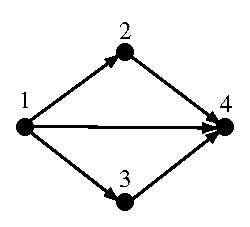
\includegraphics[scale=0.5]{graph1}
\end{center}
%
One way to represent a graph is with a dictionary \hbox{\lstinline/(vertex, vertex list) dictionary/} where
each entry in the dictionary lists the outgoing edges from that vertex.
Assume the following type definitions.

\begin{ocaml}
type vertex = int
type graph = (vertex, vertex list) dictionary
\end{ocaml}
%
Write a function \hbox{\lstinline/reachable : graph -> vertex -> vertex -> bool/}, where
\hbox{\lstinline/reachable graph v1 v2/} is \hbox{\lstinline/true/} iff vertex \hbox{\lstinline/v2/} is
reachable from \hbox{\lstinline/v1/} by following edges only in the forward direction.  Your algorithm should
terminate on all inputs.

\begin{answer}\ifanswers
To ensure that the algorithm terminates, we need to keep track of which vertices have already been
visited using a set \hbox{\lstinline/visited/} of vertices that have already been visited.  The
reachability test can be performed by a depth-first-search.

\begin{ocaml}
let reachable graph v1 v2 =
   let rec search visited v =
      if v = v2 then
         true
      else if set_mem visited v then
         false
      else
         search_list (set_insert visited v) (dict_find graph v)
   and search_list visited = function
      v :: vl -> search visited v || search_list visited vl
    | [] -> false
   in
      search set_empty v1
\end{ocaml}
\fi\end{answer}
\end{exercise}

%%%%%%%%%%%%%%%%%%%%%%%%%%%%%%%%%%%%%%%%%%%%%%%%%%%%%%%%%%%%%%%%%%%%%%%%
% Comparison
%
\begin{exercise}{set-compare}
Consider the function \hbox{\lstinline/insert/} for unbalanced, ordered, binary trees in
Section~\refsection{unbalanced-btree}.  One potential problem with this implementation is that it
uses the builtin comparison \hbox{\lstinline/(<)/}.  Rewrite the definition so the it is parameterized by a
comparison function that, given two elements, returns on of three values
%
\hbox{\lstinline/type comparison = LessThan | Equal | GreaterThan/}.
%
The expression \hbox{\lstinline/insert compare x tree/} inserts an element \hbox{\lstinline/x/} into the tree
\hbox{\lstinline/tree/}.  The type is
%
\hbox{\lstinline/insert : ('a -> 'a -> comparison) -> 'a -> 'a tree -> 'a tree/}.

\begin{answer}\ifanswers
The principal change is to use pattern matching instead of the conditional.

\begin{ocaml}
let rec insert compare x = function
   Leaf -> Node (x, Leaf, Leaf)
 | Node (y, left, right) as node ->
     match compare x y with
        LessThan -> Node (y, insert compare x left, right)
      | Equal -> node
      | GreaterThan -> Node (y, left, insert compare x right)
\end{ocaml}
\fi\end{answer}
\end{exercise}

%%%%%%%%%%%%%%%%%%%%%%%%%%%%%%%%%%%%%%%%%%%%%%%%%%%%%%%%%%%%%%%%%%%%%%%%
% Heaps
%
\begin{exercise}{heap}
A \emph{heap} of integers is a data structure supporting the following operations.

\begin{itemize}
\item \lstinline!makeheap : int -> heap!: create a heap containing a single element,
\item \lstinline!insert : heap -> int -> heap!: add an element to a heap; duplicates are allowed,
\item \lstinline!findmin : heap -> int!: return the smallest element of the heap.
\item \lstinline!deletemin : heap -> heap!: return a new heap that is the same as the original, without the smallest element.
\item \lstinline!meld : heap -> heap -> heap!: join two heaps into a new heap containing the elements of both.
\end{itemize}
%
A heap can be represented as a binary tree, where for any node $a$, if $b$ is a child node of $a$,
then $\ms{label}(a) \le \ms{label}(b)$.  The order of children does not matter.  A \emph{pairing heap} is a
particular implementation where the operations are performed as follows.

\begin{itemize}
\item \lstinline!makeheap i!: produce a single-node tree with \hbox{\lstinline/i/} at the root.
\item \lstinline!insert h i = meld h (makeheap i)!.
\item \lstinline!findmin h!: return the root label.
\item \lstinline!deletemin h!: remove the root, and \hbox{\lstinline/meld/} the subtrees.
\item \lstinline!meld h1 h2!: compare the roots, and make the heap with the larger element a subtree of the other.
\end{itemize}
%
\begin{enumerate}
\item
Define a type \hbox{\lstinline/heap/} and implement the five operations.

\begin{answer}\ifanswers
\begin{ocaml}
type heap = Node of int * heap list

let makeheap i = Node (i, [])

let meld (Node (i1, c1) as h1) (Node (i2, c2) as h2) =
   if i1 < i2 then
      Node (i1, h2 :: c1)
   else
      Node (i2, h1 :: c2)

let insert h i =
   meld h (makeheap i)

let findmin (Node (i, _)) =
   i

let deletemin = function
   Node (_, []) -> raise (Invalid_argument "deletemin")
 | Node (_, [h]) -> h
 | Node (_, h :: t) ->
     let rec meld_all h = function
        x :: t -> meld_all (meld h x) t
      | [] -> h
     in
        meld_all h t
\end{ocaml}
\fi\end{answer}

\item A \emph{heap sort} is performed by inserting the elements to be sorted into a heap,
then the values are extracted from smallest to largest.  Write a function
\hbox{\lstinline/heap_sort : int list -> int list/} that performs a heap sort,
where the result is sorted from largest to smallest.

\begin{answer}\ifanswers
\begin{ocaml}
let insert_list heap = function
   i :: elements -> insert_list (insert heap i) elements
 | [] -> heap

let heap_sort = function
   [] -> []
 | i :: elements ->
     let rec loop sorted heap =
        match heap with
           Node (i, []) -> i :: sorted
         | _ -> loop (findmin heap :: sorted) (deletemin heap)
     in
        loop [] (insert_list (makeheap i) elements)
\end{ocaml}
\fi\end{answer}
\end{enumerate}
\end{exercise}

% -*-
% Local Variables:
% Mode: LaTeX
% fill-column: 100
% TeX-master: "paper"
% TeX-command-default: "LaTeX/dvips Interactive"
% End:
% -*-
% vim:tw=100:fo=tcq:

%
%
%
\exercises

%%%%%%%%%%%%%%%%%%%%%%%%%%%%%%%%%%%%%%%%%%%%%%%%%%%%%%%%%%%%%%%%%%%%%%%%
% Reference cells.
%
\begin{exercise}{ref1}
What is the value of the following expressions?

\begin{enumerate}
\item \lstinline|let x = ref 1 in let y = x in y := 2; !x|

\begin{answer}\ifanswers
The variables \hbox{\lstinline/x/} and \hbox{\lstinline/y/} refer to the same reference cell, so the result is \hbox{\lstinline/2/}.
\fi\end{answer}

\item \lstinline|let x = ref 1 in let y = ref 1 in y := 2|

\begin{answer}\ifanswers
The variables \hbox{\lstinline/x/} and \hbox{\lstinline/y/} refer to different reference cells, so the result is \hbox{\lstinline/1/}.
\fi\end{answer}

\item

\begin{ocamllisting}
let x = ref 1 in
let y = ref x in
!y := 2;
!x
\end{ocamllisting}

\begin{answer}\ifanswers
Since \hbox{\lstinline/y/} refers to \hbox{\lstinline/x/}, assigning to \hbox{\lstinline/!y/} is the same as assigning to \hbox{\lstinline/x/}.
The final value \hbox{\lstinline/!x/} is \hbox{\lstinline/2/}.
\fi\end{answer}

\item

\begin{ocamllisting}
let fst (x, _) = x in
let snd (_, x) = x in
let y = ref 1 in
let x = (y, y) in
fst x := 2;
!(snd x)
\end{ocamllisting}

\begin{answer}\ifanswers
Both elements of the pair \hbox{\lstinline/(y, y)/} refer to the same cell, so the assignment \hbox{\lstinline/fst x := 2/}
effects both parts; the value \hbox{\lstinline/!(snd x)/} is \hbox{\lstinline/2/}.
\fi\end{answer}

\item

\begin{ocamllisting}
let x = ref 0 in
let y = ref [5; 7; 2; 6] in
while !y <> [] do
   x := !x + 1;
   y := List.tl !y
done;
!x
\end{ocamllisting}

\begin{answer}\ifanswers
The variable \hbox{\lstinline/x/} is incremented for each element of the list \hbox{\lstinline/y/}, so the final
value \hbox{\lstinline/!x/} is \hbox{\lstinline/4/}.
\fi\end{answer}

\end{enumerate}
\end{exercise}

%%%%%%%%%%%%%%%%%%%%%%%%%%%%%%%%%%%%%%%%%%%%%%%%%%%%%%%%%%%%%%%%%%%%%%%%
% Lazy values
%
\begin{exercise}{lazy}
\label{keyword:lazy}
\index{lazy value}
A \emph{lazy} value is a computation that is deferred until it is needed; we say that it is
\emph{forced}.  A forced value is memoized, so that subsequent forcings do not reevaluate the
computation.  The OCaml standard library already provides an implementation of lazy values in the
\hbox{\lstinline/Lazy/} module, but we can also construct them ourselves using reference cells and
functions.

\begin{ocaml}
type 'a deferred
val defer : (unit -> 'a) -> 'a deferred
val force : 'a deferred -> 'a
\end{ocaml}
%
Implement the type \hbox{\lstinline/'a deferred/} and the functions \hbox{\lstinline/defer/} and \hbox{\lstinline/force/}.

\begin{answer}\ifanswers
The important part is that the forcing is memoized.  We can use a reference cell to save to computation.

\begin{ocaml}
type 'a deferred_value =
   Deferred of (unit -> 'a)
 | Forced of 'a

type 'a deferred = 'a deferred_value ref

let defer f = ref (Deferred f)

let force cell =
   match !cell with
      Deferred f ->
         let result = f () in
         cell := Forced result;
         result
    | Forced result ->
         result
\end{ocaml}
\fi\end{answer}
\end{exercise}

%%%%%%%%%%%%%%%%%%%%%%%%%%%%%%%%%%%%%%%%%%%%%%%%%%%%%%%%%%%%%%%%%%%%%%%%
% Lazy lists
%
\begin{exercise}{lazy-list}
\index{lazy list}
A lazy list is a list where the tail of the list is a deferred computation (a lazy list is also
called a \emph{stream}).  The type can be defined as follows, where the type \hbox{\lstinline/deferred/} is
defined as in Exercise~\ref{exercise:lazy}.

\begin{ocaml}
type 'a lazy_list =
   Nil
 | Cons of 'a * 'a lazy_list
 | LazyCons of 'a * 'a lazy_list deferred
\end{ocaml}
%
Define the following functions on lazy lists.

\begin{ocamlx}
val nil       : 'a lazy_list
val cons      : 'a -> 'a lazy_list -> 'a lazy_list
val lazy_cons : 'a -> (unit -> 'a lazy_list) -> 'a lazy_list
val is_nil    : 'a lazy_list -> bool
val head      : 'a lazy_list -> 'a
val tail      : 'a lazy_list -> 'a lazy_list
val (@@)      : 'a lazy_list -> 'a lazy_list -> 'a lazy_list
\end{ocamlx}
%
The expression \hbox{\lstinline/$l_1$ @@ $l_2$/} appends two lazy lists in constant time.

\begin{answer}\ifanswers
The implementations are as follows.

\begin{ocamlx}
let nil = Nil
let cons h t = Cons (h, t)
let lazy_cons h f = LazyCons (h, defer f)

let is_nil = function
   Nil -> true
 | Cons _ | LazyCons _ -> false

let head = function
   Nil -> raise (Invalid_argument "head")
 | Cons (h, _)
 | LazyCons (h, _) -> h

let tail = function
   Nil -> raise (Invalid_argument "tail")
 | Cons (_, t) -> t
 | LazyCons (_, f) -> force f

let rec (@@) l1 l2 =
   match l1, l2 with
      Nil, l | l, Nil -> l
    | _ -> lazy_cons (head l1) (fun () -> tail l1 @@ l2)
\end{ocamlx}
\fi\end{answer}
\end{exercise}

%%%%%%%%%%%%%%%%%%%%%%%%%%%%%%%%%%%%%%%%%%%%%%%%%%%%%%%%%%%%%%%%%%%%%%%%
% Queues.
%
\begin{exercise}{fun-queue}
\index{queue!functional}
The FIFO queues described in Section~\ref{section:queues} are imperative; whenever a value is added to
or taken from the queue, the queue is modified by side-effect.  Implement a \emph{persistent} queue
with the following operations.

\begin{ocaml}
val empty : 'a queue
val add   : 'a queue -> 'a -> 'a queue
val take  : 'a queue -> 'a * 'a queue
\end{ocaml}
%
The expression \hbox{\lstinline/add queue e/} produces a new queue, without affecting the contents of the
original queue \hbox{\lstinline/queue/}.  The expression \hbox{\lstinline/take queue/} returns an element of the
queue \hbox{\lstinline/queue/} and a new queue; again, the contents of the original queue \hbox{\lstinline/queue/}
are unaffected.

$\star$ Can you implement the queue so that any sequence of $n$ \hbox{\lstinline/add/} and \hbox{\lstinline/take/}
operations, in any order, take $O(n)$ time?  Hint: consider using lazy lists
(Exercise~\ref{exercise:lazy-list}) to represent the queue, shifting the queue whenever the
$\ms{front}$ is longer than the $\ms{back}$.  See Okasaki~\cite{Oka95}.

\begin{answer}\ifanswers
The queue could simply be represented as a list, but then one of the operations \hbox{\lstinline/add/} or
\hbox{\lstinline/take/} would take time $O(m)$ where $m$ is the length of the queue.

The two list \hbox{\lstinline/($\ms{front}$, $\ms{back}$)/} representation is a little better.  To make the
data structure persistent, the functions \hbox{\lstinline/add/} and \hbox{\lstinline/take/} produce new queues.

\begin{ocamlnum}
type 'a queue = ('a list * 'a list) ref

let empty = ref ([], [])

let add queue x =
   let (front, back) = !queue in
   ref (x :: front, back)

let rec take queue =
   match !queue with
      [], [] -> raise (Invalid_argument "queue")
    | front, x :: back ->
        x, ref (front, back)
    | front, [] ->
        queue := ([], List.rev front);
        take queue
\end{ocamlnum}
%
The side effect on line 15 does not affect persistence because the queue membership is preserved.
However, efficiency is still not optimal.  Consider a sequence of $m$ \hbox{\lstinline/add/}s, followed by $m$ \hbox{\lstinline/take/}s.

\begin{ocaml}
let $q_1$ = add empty 1
let $q_2$ = add $q_1$ 2
...
let $q_m$ = add $q_{m - 1}$ $m$
let $x_m$, _ = take $q_m$
let $x_{m - 1}$, _ = take $q_{m - 1}$
...
let $x_1$, _ = take $q_1$
\end{ocaml}
%
Each operation \hbox{\lstinline/take $q_i$/} shifts $i$ elements of the queue, so the total time is $O(m^2)$.

Okasaki gives an efficient implementation, summarized below in OCaml.  A function
\hbox{\lstinline/maybe_shift/} is used to shift the queue whenever the front becomes longer than the back.
The list lengths are needed, so the queue is a 4-tuple
%
\hbox{\lstinline/($\ms{front}$, $|\ms{front}|$, $\ms{back}$, $|\ms{back}|$)/}.

\begin{ocaml}
type 'a queue = 'a lazy_list * int * 'a lazy_list * int

let empty = (Nil, 0, Nil, 0)

let insert (front, flen, back, blen) x =
   maybe_shift (cons x front) (flen + 1) back blen

let remove (front, flen, back, blen) =
   head back, maybe_shift front flen (tail back) (blen - 1)

let maybe_shift front flen back blen =
   if flen <= blen then
      (front, flen, back, blen)
   else
      (Nil, 0, shift front back [], flen + blen)

let shift front back l =
   if is_nil back then
      cons (head front) l
   else
      lazy_cons (head back) (fun () ->
         shift (tail front) (tail back) (cons (head front) l))
\end{ocaml}
\fi\end{answer}
\end{exercise}

%%%%%%%%%%%%%%%%%%%%%%%%%%%%%%%%%%%%%%%%%%%%%%%%%%%%%%%%%%%%%%%%%%%%%%%%
% Memoization
%
\begin{exercise}{memoization}
\index{memoization!of recursive functions}
One problem with the memoization function \hbox{\lstinline/memo : ('a -> 'b) -> ('a -> 'b)/} in
Section~\ref{section:memoization} is that it ignores recursive definitions.  For example,
the expression \hbox{\lstinline/memo fib $i$/} still takes exponential time in $i$ to compute.

To solve this, we'll need to modify the recursive definition for \hbox{\lstinline/fib/} and perform an
explicit memoization.  Implement the following types and functions, where
%
\hbox{\lstinline/fib = memo_fib (create_memo ())/}.  How fast is the Fibonacci function now?

\begin{ocaml}
type ('a, 'b) memo
val create_memo : unit -> ('a, 'b) memo
val memo_find   : ('a, 'b) memo -> 'a -> 'b option
val memo_add    : ('a, 'b) memo -> 'a -> 'b -> unit
val memo_fib    : (int, int) memo -> int -> int

let fib = memo_fib (create_memo ())
\end{ocaml}

\begin{answer}\ifanswers
The main task here is to separate the parts of the memoization.  We'll use a simple association list
for the memo table.  The expression \hbox{\lstinline/fib $n$/} is computed in quadratic time $O(n^2)$.  A
more efficient implementation of the dictionary would reduct this to no more than $O(n \log n)$
time.

\begin{ocaml}
type ('a, 'b) memo = ('a * 'b) list

let create_memo () = []

let rec memo_find table x =
   match table with
      (x', y) :: _ when x' = x -> Some y
    | _ :: table -> memo_find table x
    | [] -> None

let memo_fib table i =
   match memo_find table i with
      Some j -> j
    | None -> 
        match i with
           0 | 1 -> i
         | _ ->
            let j = memo_fib table (i - 1) + memo_fib table (i - 2) in
            memo_add table i j;
            j
\end{ocaml}
\fi\end{answer}
\end{exercise}

%%%%%%%%%%%%%%%%%%%%%%%%%%%%%%%%%%%%%%%%%%%%%%%%%%%%%%%%%%%%%%%%%%%%%%%%
% Directed graphs
%
\begin{exercise}{dfs}
\index{depth-first search}
One way to represent a directed graph is with an adjacency list stored directly in each vertex.
Each vertex has a label and a list of out-edges; we also include a ``mark'' flag and an integer to
be used by a depth-first-search.

\begin{ocaml}
type 'a vertex =
   (* Vertex (label, out-edges, dfs-mark, dfs-index) *)
   Vertex of 'a * 'a vertex list ref * bool ref * int option ref

type 'a directed_graph = 'a vertex list
\end{ocaml}
%
Depth-first search and breadth-first search are two highly useful graph algorithms.
A depth-first search (DFS) traverses the graph, assigning to each vertex a DFS index and
marking a vertex $v$ when all out-edges of $v$ have been explored.  The DFS search is performed as follows.

Choose an unmarked vertex $u$ in the graph, push out-edges $(u, v)$ onto a stack.  Assign $u$ DFS index 0, set
the DFS counter $c$ to 1, and then repeat the following until the stack is empty.

\begin{enumerate}
\item Pop an edge $(u, v)$ from the stack, and classify it according to the following
table.

\begin{center}
\begin{tabular}{l|l}
Condition & Edge type for $(u, v)$\\
\hline
$v$ does not have a DFS index & tree edge\\
$\ms{DFS}(u) < \ms{DFS}(v)$ & forward edge\\
$\ms{DFS}(u) > \ms{DFS}(v)$ and $v$ not marked & back edge\\
$\ms{DFS}(u) > \ms{DFS}(v)$ and $v$ marked & cross edge
\end{tabular}
\end{center}
%
\item
If $(u, v)$ is a tree edge, assign $v$ the current DFS index $c$, increment $c$, and push all edges
$(v, w)$ onto the stack.
\item
When all edges $(u, v)$ have been considered, mark the vertex $u$.
\end{enumerate}
%
Repeat until all vertices have been marked.
A graph is \emph{cyclic} iff the DFS search found any back-edges.

Implement a DFS search.  You can assume that all vertices are initially unmarked and their DFS index
is \hbox{\lstinline/None/}.

\begin{answer}\ifanswers
We'll keep a flag \hbox{\lstinline/cyclic/} to indicate whether the graph is cyclic.  First, all the mark
bits and DFS counters are cleared, then the function \hbox{\lstinline/search/} is called to perform the DFS
search.  It isn't necessary to keep an explicit stack of edges---in effect, the OCaml runtime stack
is serving as the edge stack.

\begin{ocaml}
let rec dfs graph =
   let cyclic = ref false in
   let dfs_counter = ref 0 in

   (* The main DFS search *)
   let rec search (Vertex (_, u_edges, u_mark, u_index)) =
      if not !u_mark then begin
         let c = !dfs_counter in
         u_index := Some c;
         dfs_counter := c + 1;
         List.iter (fun (Vertex (_, _, v_mark, v_index) as v) ->
            match !v_index with
               Some index ->
                  if index < c && not !v_mark then
                     cyclic := true
             | None ->
                  search v) !u_edges;
         u_mark := true
      end
   in

   (* Reset the graph state *)
   List.iter (fun (Vertex (_, _, mark, index)) ->
      mark := false;
      index := None) graph;

   (* DFS over all the vertices in the graph *)
   List.iter search graph
\end{ocaml}
\fi\end{answer}
\end{exercise}

%%%%%%%%%%%%%%%%%%%%%%%%%%%%%%%%%%%%%%%%%%%%%%%%%%%%%%%%%%%%%%%%%%%%%%%%
% Copying
%
\begin{exercise}{graph-map}
One issue with graph data structures is that some familiar operations are hard to implement.  For
example, consider the following representation (similar to the previous exercise) for a directed graph.

\begin{ocaml}
(* Vertex (label, out-edges) *)
type 'a vertex = Vertex of 'a * 'a vertex list ref
type 'a directed_graph = 'a vertex list
\end{ocaml}
%
Suppose we want to define a polymorphic map function on graphs.

\begin{ocaml}
val graph_map : ('a -> 'b) -> 'a directed_graph -> 'b directed_graph
\end{ocaml}
%
Given an arbitrary function \hbox{\lstinline/f : 'a -> 'b/} and a graph \hbox{\lstinline/g/}, the expression
\hbox{\lstinline/graph_map f g/} should produce a graph isomorphic to \hbox{\lstinline/g/}, but where
\hbox{\lstinline/f/} has been applied to each label.  Is the function \hbox{\lstinline/graph_map/} definable?  If
so, describe the implementation.  If not, explain why not.  Is there another implementation of
graphs where \hbox{\lstinline/graph_map/} can be implemented efficiently?

\begin{answer}\ifanswers
The function \hbox{\lstinline/graph_map/} is definable, but it is difficult to implement it efficiently.
The central issue is that, in order to preserve the structure of the graph, the function
\hbox{\lstinline/graph_map/} must be memoized using physical equality.  The following code gives a simple,
but inefficient, implementation.

\begin{ocamlnum}
let graph_map f graph =
   let memo = ref [] in
   let rec map u = function
      (u', v) :: table when u' == u -> v
    | _ :: table -> map u table
    | [] ->
       let (label, out_edges) = u in
       let new_out_edges = ref [] in
       let new_u = (f label, new_out_edges) in
       memo := (u, new_u) :: !memo;
       new_out_edges := map_list !out_edges
   and map_list edges =
      List.map (fun v -> map v !memo) edges
   in
   map_list graph
\end{ocamlnum}
%
The function \hbox{\lstinline/map/} searches through the memo table in linear order, looking for an entry
that matches with physical equality (\hbox{\lstinline/==/}).  If so, the previous result is returned.
Otherwise, a new vertex is created and added to the memo table.  Note that the new vertex
\hbox{\lstinline/new_u/} is added before following the out-edges recursively, preventing infinite looping
on cyclic graphs.

Given a graph with $n$ vertices and $m$ edges, the function \hbox{\lstinline/map/} examines $n$ vertices worst case, so the total time complexity is of \hbox{\lstinline/graph_map/} is $O(nm)$.

An alternative representation that would support an efficient map is to give vertices unique names,
and refer to them by name rather than referring to them directly.  The penalty is that edge
traversal takes time $O(\log n)$ rather than constant time because of the dictionary lookup.

\begin{ocaml}
(* A name for a vertex *)
type name = int

(* A vertex is (label, out-edges) *)
type 'a vertex = 'a * name list ref

(* A graph is (vertices, vertex dictionary) *)
type 'a graph = name list * (name, 'a vertex) dictionary

let graph_map f (vertices, dict) =
   vertices, dictionary_map f dict
\end{ocaml}
\fi\end{answer}
\end{exercise}

% -*-
% Local Variables:
% Mode: LaTeX
% fill-column: 100
% TeX-master: "paper"
% TeX-command-default: "LaTeX/dvips Interactive"
% End:
% -*-
% vim:tw=100:fo=tcq:

%
%
%
\exercises

%%%%%%%%%%%%%%%%%%%%%%%%%%%%%%%%%%%%%%%%%%%%%%%%%%%%%%%%%%%%%%%%%%%%%%%%
% Reference cells
%
\begin{exercise}{ref-record}
Reference cells are a special case of records, with the following type definition.

\begin{ocaml}
type 'a ref = { mutable contents : 'a }
\end{ocaml}
%
Implement the operations on reference cells.

\begin{ocaml}
val ref  : 'a -> 'a ref
val (!)  : 'a ref -> 'a
val (:=) : 'a ref -> 'a -> unit
\end{ocaml}

\begin{answer}\ifanswers
The operations are implemented with operations on records.

\begin{ocaml}
let ref x = { contents = x }
let (!) cell = cell.contents
let (:=) cell x = cell.contents <- x
\end{ocaml}
\fi\end{answer}
\end{exercise}

%%%%%%%%%%%%%%%%%%%%%%%%%%%%%%%%%%%%%%%%%%%%%%%%%%%%%%%%%%%%%%%%%%%%%%%%
% Value restriction.
%
\begin{exercise}{record-value-restriction}
Consider the following record type definition.

\begin{ocaml}
type ('a, 'b) mpair = { mutable fst : 'a; snd : 'b }
\end{ocaml}
%
What are the types of the following expressions?

\begin{enumerate}
\item \lstinline$[|[]|]$

\begin{answer}\ifanswers
The type is \hbox{\lstinline/[|[]|] : '_a list array/}.
\fi\end{answer}

\item \lstinline+{ fst = []; snd = [] }+

\begin{answer}\ifanswers
Mutable fields are not values, so the field \hbox{\lstinline/fst/} is not polymorphic because of the value restriction.
The type is \hbox{\lstinline/{ fst = []; snd = [] } : ('_a list, 'b list) mpair/}.
\fi\end{answer}

\item \lstinline+{ { fst = (); snd = 2 } with fst = 1 }+

\begin{answer}\ifanswers
During a functional update, it is legal for the types of polymorphic fields to change.
The expression \hbox{\lstinline/{ fst = (); snd = 2 }/} has type \hbox{\lstinline/(unit, int) mpair/},
but the final value is \hbox{\lstinline/{ fst = 1; snd = 2 }/} of type \hbox{\lstinline/(int, int) mpair/}.
\fi\end{answer}
\end{enumerate}
\end{exercise}

%%%%%%%%%%%%%%%%%%%%%%%%%%%%%%%%%%%%%%%%%%%%%%%%%%%%%%%%%%%%%%%%%%%%%%%%
% ADTs
%
\begin{exercise}{record-adt}
Records can be used to implement abstract data structures, where the data structure is viewed as
a record of functions, and the data representation is hidden.  For example, a type definition for a
functional dictionary is as follows.

\begin{ocaml}
type ('key, 'value) dictionary =
   { insert : 'key -> 'value -> ('key, 'value) dictionary;
     find   : 'key -> 'value
   }

val empty : ('key, 'value) dictionary
\end{ocaml}
%
Implement the empty dictionary \hbox{\lstinline/empty/}.  Your implementation should be pure, without side-effects.
You are free to use any internal representation of the dictionary.

\begin{answer}\ifanswers
We'll use association lists.  The function \hbox{\lstinline/insert/} adds to the list, and \hbox{\lstinline/find/}
searches the list.  The function \hbox{\lstinline/new_dictionary/} is used to form a dictionary from
an association list.

\begin{ocaml}
let empty =
   let rec find entries key =
      match entries with
         (key', value) :: _ when key' = key -> value
       | _ :: entries -> find entries key
       | [] -> raise Not_found
   in
   let rec new_dictionary entries =
      { insert = insert entries;
        find = find entries
      }
   and insert entries key value =
      new_dictionary ((key, value) :: entries)
   in
   new_dictionary []
\end{ocaml}
\fi\end{answer}
\end{exercise}

%%%%%%%%%%%%%%%%%%%%%%%%%%%%%%%%%%%%%%%%%%%%%%%%%%%%%%%%%%%%%%%%%%%%%%%%
% Objects
%
\begin{exercise}{record-objects1}
Records can also be used to implement a simple form of object-oriented programming.  Suppose we are
implementing a collection of geometric objects (blobs), where each blob has a position, a function (called a \emph{method}) to
compute the area covered by the blob, and methods to set the position and move the blob.  The
following record defines the methods for a generic object.

\begin{ocaml}
type blob =
   { get    : unit -> float * float;
     area   : unit -> float;
     set    : float * float -> unit;
     move   : float * float -> unit
   }
\end{ocaml}
%
An actual object like a rectangle might be defined as follows.

\begin{ocaml}
let new_rectangle x y w h =
   let pos = ref (x, y) in
   let rec r =
      { get  = (fun () -> !pos);
        area = (fun () -> w *. h);
        set  = (fun loc -> pos := loc);
        move = (fun (dx, dy) ->
                   let (x, y) = r.get () in
                   r.set (x +. dx, y +. dy))
      }
   in
   r
\end{ocaml}
%
The rectangle record is defined recursively so that the method \hbox{\lstinline/move/} can be defined in
terms of \hbox{\lstinline/get/} and \hbox{\lstinline/set/}.

Suppose we have created a new rectangle \hbox{\lstinline/rect1/}, manipulated it, and now we want to fix it
in position.  We might try to do this by redefining the method \hbox{\lstinline/set/}.

\begin{ocaml}
let rect1 = new_rectangle 0.0 0.0 1.0 1.0 in
rect1.move 1.2 3.4; $\cdots$
let rect2 = { rect1 with set = (fun _ -> ()) }
\end{ocaml}
%
\begin{enumerate}
\item What happens to \hbox{\lstinline/rect2/} when \hbox{\lstinline/rect2.move/} is called?  How can you prevent it from moving?
\item What happens to \hbox{\lstinline/rect2/} when \hbox{\lstinline/rect1.set/} is called?
\end{enumerate}

\begin{answer}\ifanswers
The problem is that the method \hbox{\lstinline/move/} refers to the definitions of \hbox{\lstinline/get/} and
\hbox{\lstinline/set/} when the rectangle is first created.  This is called \emph{early binding}, where
true object systems use \emph{late} binding.  Early binding means that the method \hbox{\lstinline/move/}
is not updated when \hbox{\lstinline/set/} is changed.

\begin{enumerate}
\item
The expression \hbox{\lstinline/rect2.move (dx, dy)/} moves \hbox{\lstinline/rect2/} by \hbox{\lstinline/(dx, dy)/}.  To
prevent this from happening, the method \hbox{\lstinline/move/} should be updated as well.

\begin{ocaml}
let rect2 = { rect1 with set = (fun _ -> ()); move = (fun _ -> ()) }
\end{ocaml}

\item The rectangles \hbox{\lstinline/rect2/} and \hbox{\lstinline/rect1/} refer to the same position \hbox{\lstinline/pos/},
so setting the position of \hbox{\lstinline/rect1/} also moves \hbox{\lstinline/rect2/}.
\end{enumerate}
\fi\end{answer}
\end{exercise}

%%%%%%%%%%%%%%%%%%%%%%%%%%%%%%%%%%%%%%%%%%%%%%%%%%%%%%%%%%%%%%%%%%%%%%%%
% Array reversal
%
\begin{exercise}{reverse}
Write a function \hbox{\lstinline/string_reverse : string -> unit/} to reverse a string in-place.

\begin{answer}\ifanswers
\begin{ocaml}
let string_reverse s =
   let len = String.length s in
   for i = 0 to len / 2 - 1 do
      let c = s.[i] in
      s.[i] <- s.[len - i - 1];
      s.[len - i - 1] <- c
   done
\end{ocaml}
\fi\end{answer}
\end{exercise}

%%%%%%%%%%%%%%%%%%%%%%%%%%%%%%%%%%%%%%%%%%%%%%%%%%%%%%%%%%%%%%%%%%%%%%%%
% Blit
%
\begin{exercise}{blit}
What problem might arise with the following implementation of an array blit function?
How can it be fixed?

\begin{ocaml}
let blit src src_off dst dst_off len =
   for i = 0 to len - 1 do
      dst.(dst_off + i) <- src.(src_off + i)
   done
\end{ocaml}

\begin{answer}\ifanswers
There can be a problem if the \hbox{\lstinline/src/} and \hbox{\lstinline/dst/} arrays are the same,
and the ranges to be copied overlap, and \hbox{\lstinline/dst_off > src_off/}.

For example, the following expression duplicates the first element of the array
instead of copying a subrange.

\begin{ocaml}
let data = [|1; 2; 3; 4; 5; 6; 7; 8; 9|];;
@
\begin{topoutput}
val data : int array = [|1; 2; 3; 4; 5; 6; 7; 8; 9|]
\end{topoutput}
@
# blit data 0 data 1 5;;
@
\begin{topoutput}
- : unit = ()
\end{topoutput}
@
# data;;
@
\begin{topoutput}
- : int array = [|1; 1; 1; 1; 1; 1; 7; 8; 9|]
\end{topoutput}
@
\end{ocaml}
%
An easy solution is to copy in reverse direction when \hbox{\lstinline/dst_off > src_off/}.

\begin{ocaml}
let blit src src_off dst dst_off len =
   if dst_off < src_off then
      for i = 0 to len - 1 do
         dst.(dst_off + i) <- src.(src_off + i)
      done
   else
      for i = len - 1 downto 0 do
         dst.(dst_off + i) <- src.(src_off + i)
      done
\end{ocaml}
\fi\end{answer}
\end{exercise}

%%%%%%%%%%%%%%%%%%%%%%%%%%%%%%%%%%%%%%%%%%%%%%%%%%%%%%%%%%%%%%%%%%%%%%%%
% Insertion sort
%
\begin{exercise}{insertion-sort}
\index{insertion sort}

\emph{Insertion sort}
is a sorting algorithm that works by inserting elements one-by-one
into an array of sorted elements.  Although the algorithm takes
$O(n^2)$ time to sort an array of $n$ elements, it is simple, and it
is also efficient when the array to be sorted is small.  The
pseudo-code is as follows.

\begin{ccode}
insert(array a, int i)
    x <- a[i]
    j <- i - 1
    while j >= 0 and a[j] > x
        a[j] <- a[j - 1]
        j = j - 1
    a[j + 1] <- x

insertion_sort(array a)
    i <- 1
    while i < length(a)
        insert(a, i)
        i <- i + 1
\end{ccode}
%
Write this program in OCaml.

\begin{answer}\ifanswers
Each of the constructs in the pseudo-code can be translated directly to OCaml.  However, it is
slightly more efficient to avoid the use of reference cells, and translate the while-loop as a
recursive function.

\begin{ocaml}
let insert a i =
   let x = a.(i) in
   let rec loop j =
      if j >= 0 && a.(j) > x then begin
         a.(j) <- a.(j - 1);
         loop (j - 1)
      end
      else
         j
   in
   let j = loop (i - 1) in
   a.(j) <- x

and insertion_sort a =
   for i = 1 to Array.length a - 1 do
      insert a i
   done
\end{ocaml}
\fi\end{answer}
\end{exercise}

% -*-
% Local Variables:
% Mode: LaTeX
% fill-column: 100
% TeX-master: "paper"
% TeX-command-default: "LaTeX/dvips Interactive"
% End:
% -*-
% vim:tw=100:fo=tcq:

%
%
%
\exercises

%%%%%%%%%%%%%%%%%%%%%%%%%%%%%%%%%%%%%%%%%%%%%%%%%%%%%%%%%%%%%%%%%%%%%%%%
% Exercise
%
\begin{exercise}{exn1}
Which of the following are legal expressions?

\begin{enumerate}
\item \lstinline+exception A+
\item \lstinline+exception b+
\item \lstinline+exception C of string+
\item \lstinline+exception D of exn+
\item \lstinline+exception E of exn let x = E (E (E Not_found))+
\item \lstinline+let f () = exception F raise F+
\end{enumerate}

\begin{answer}\ifanswers
\begin{enumerate}
\item \lstinline+exception A+ is legal.
\item \lstinline+exception b+ is not legal because the name \lstinline+b+ must be capitalized.
\item \lstinline+exception C of string+ is legal.
\item \lstinline+exception D of exn+ is legal, it adds a recursive definition.
\item \lstinline+exception E of exn let x = E (E (E Not_found))+ is also legal, the value \lstinline+x+ has type \lstinline+exn+.
\item \lstinline+let f () = exception F raise F+ is not legal, exceptions can only be declared at the top-level, not
within function bodies.
\end{enumerate}
\fi\end{answer}
\end{exercise}

%%%%%%%%%%%%%%%%%%%%%%%%%%%%%%%%%%%%%%%%%%%%%%%%%%%%%%%%%%%%%%%%%%%%%%%%
% Exercise
%
\begin{exercise}{exn2}
What is the result of evaluating the following programs?

\begin{enumerate}
\item

\begin{ocamllisting}
exception A
try raise A with
   A -> 1
\end{ocamllisting}

\item

\begin{ocamllisting}
exception A of int
let f i =
   raise (A (100 / i));;
let g i =
   try f i with
      A j -> j;;
g 100
\end{ocamllisting}

\item

\begin{ocamllisting}
exception A of int
let rec f i =
   if i = 0 then
      raise (A i)
   else
      g (i - 1)
and g i =
   try f i with
      A i -> i + 1;;
g 2
\end{ocamllisting}
\end{enumerate}

\begin{answer}\ifanswers
\begin{enumerate}
\item 1

\item

When \lstinline+g+ is called, \lstinline+f+ is called with the argument \lstinline+100+, raising the
exception \lstinline+A 1+, passing control back to \lstinline+g+ which returns \lstinline+1+.

\item

The expression \lstinline+g i+ returns 1 for any value $\texttt{i} \ge 0$.  The function \lstinline+f+ always
raises the exception \lstinline+A 0+, which passes control to the \emph{innermost} exception handler for
\lstinline+g+, which then returns 1.  As the call stack unwinds, the return value \lstinline+1+ is passed unchanged.

\end{enumerate}
\fi\end{answer}
\end{exercise}

%%%%%%%%%%%%%%%%%%%%%%%%%%%%%%%%%%%%%%%%%%%%%%%%%%%%%%%%%%%%%%%%%%%%%%%%
% Exercise
%
\begin{exercise}{exn3}
In the following program, the function \lstinline+sum_entries+ sums up the integer values associated with
each name in the list \lstinline+names+.  The \lstinline+List.assoc+ function finds the value associated with
the name, raising the \lstinline+Not_found+ exception if the entry is not found.  For example, the
expression \lstinline+sum_entries 0 ["a"; "c"]+ would evaluate to \lstinline+35+, and the expression
\lstinline+sum_entries 0 ["a"; "d"]+ would raise the \lstinline+Not_found+ exception.

\begin{center}
\begin{ocaml}
let table = [("a", 10); ("b", 20); ("c", 25)]
let rec sum_entries total (names : string list) =
   match names with
      name :: names' ->
         sum_entries (total + List.assoc name table) names'
    | [] ->
         total
\end{ocaml}
\end{center}
%
Suppose we wish to catch the exception, arbitrarily assigning a value of 0 to each unknown entry.
What is the difference between the following two functions?  Which form is preferable?

\begin{enumerate}
\item 
\begin{center}
\begin{ocaml}
let table = [("a", 10); ("b", 20); ("c", 25)]
let rec sum_entries total (names : string list) =
   match names with
      name :: names' ->
         (try sum_entries (total + List.assoc name table) names' with
             Not_found ->
                sum_entries total names')
    | [] ->
         total
\end{ocaml}
\end{center}

\item
\begin{center}
\begin{ocaml}
let table = [("a", 10); ("b", 20); ("c", 25)]
let rec sum_entries total (names : string list) =
   match names with
      name :: names' ->
         let i =
            try List.assoc name table with
               Not_found  ->
                  1
         in
            sum_entries (total + i) names'
    | [] ->
         total
\end{ocaml}
\end{center}
\end{enumerate}

\begin{answer}\ifanswers
The second form is preferable.  The first version is not tail-recursive, and the depth of the
exception stack is linear in the number of entries in the \lstinline+names+ list.  The second version
does not have these problems; it is properly tail-recursive.
\fi\end{answer}
\end{exercise}

%%%%%%%%%%%%%%%%%%%%%%%%%%%%%%%%%%%%%%%%%%%%%%%%%%%%%%%%%%%%%%%%%%%%%%%%
% Exercise
%
\begin{exercise}{exn4}
Suppose we are given a \lstinline+table+ as in the last exercise, and we wish to call some function
\lstinline+f+ on one of the entries, or returning 0 if the entry is not found.  That is, we are given the
function \lstinline+f+, and a name, and we wish to evaluate \lstinline+f (List.assoc table name)+.  What is
the difference between the following functions?

\begin{enumerate}
\item 
\begin{center}
\begin{ocaml}
let callf f name =
   try f (List.assoc table name) with
      Not_found ->
         0
\end{ocaml}
\end{center}

\item
\begin{center}
\begin{ocaml}
let callf f name =
   let i =
      try Some (List.assoc table name) with
         Not_found ->
            None
   in
      match i with
         Some j -> f j
       | None -> 0
\end{ocaml}
\end{center}
\end{enumerate}

\begin{answer}\ifanswers
In the first version, the function \lstinline+f+ is called within the exception handler, which means that
if \lstinline+f+ raises the \lstinline+Not_found+ exception, then \lstinline+callf+ will return 0, the same as if
the \lstinline+List.assoc+ function raises \lstinline+Not_found+.

The second version separates the calls.  If the function \lstinline+f+ raises \lstinline+Not_found+, the
exception will be propagated through the calls to \lstinline+callf+.  The second form is preferable in
situations where exceptions raised from \lstinline+f+ indicate an error, not normal operation.
\fi\end{answer}
\end{exercise}

%%%%%%%%%%%%%%%%%%%%%%%%%%%%%%%%%%%%%%%%%%%%%%%%%%%%%%%%%%%%%%%%%%%%%%%%
% Exercise
%
\begin{exercise}{exn5}
The expression \lstinline+input_line stdin+ reads a line of text from standard input, returning the line
as a string, or raising the exception \lstinline+End_of_file+ if the end of the file has been reached.
Write a function \lstinline+input_lines+ to read all the lines from the channel \lstinline+stdin+, returning a
list of all the lines.  The order of the lines in the list does not matter.

\begin{answer}\ifanswers
The main problem with writing the \lstinline+input_lines+ function is in catching the \lstinline+End_of_file+ exception.
The following program is inefficient, because the exception stack is linear in the length of the input file.
For large files, the stack will likely overflow.

\begin{center}
\begin{ocaml}
let rec input_lines stdin =
    try input_line stdin :: input_lines stdin with
       End_of_file ->
          []
\end{ocaml}
\end{center}
%
The way to code this efficiently is to wrap the \lstinline+input_line+ function to catch the exception.

\begin{center}
\begin{ocaml}
let maybe_input_line stdin =
   try Some (input_line stdin) with
      End_of_file ->
         None

let input_lines stdin =
   let rec input lines =
      match maybe_input_line stdin with
         Some line -> input (line :: lines)
       | None -> List.rev lines
   in
      input []
\end{ocaml}
\end{center}
\fi\end{answer}
\end{exercise}

% -*-
% Local Variables:
% Mode: LaTeX
% fill-column: 100
% TeX-master: "paper"
% TeX-command-default: "LaTeX/dvips Interactive"
% End:
% -*-
% vim:tw=100:fo=tcq:

%
%
%

\exercises

%%%%%%%%%%%%%%%%%%%%%%%%%%%%%%%%%%%%%%%%%%%%%%%%%%%%%%%%%%%%%%%%%%%%%%%%
% Exercise
%
\begin{exercise}{helloworld}
Write a ``Hello world'' program, which prints the
line \hbox{\lstinline+Hello world!+} to the standard output.

\begin{answer}\ifanswers
The \hbox{\lstinline+output_string+} function can be used to print the
line.

\begin{ocaml}
# output_string stdout "Hello world!\n";;
@
\begin{topoutput}
Hello world
\end{topoutput}
@
\end{ocaml}
\fi\end{answer}
\end{exercise}

%%%%%%%%%%%%%%%%%%%%%%%%%%%%%%%%%%%%%%%%%%%%%%%%%%%%%%%%%%%%%%%%%%%%%%%%
% Exercise
%
\begin{exercise}{ioexn1}
The input functions raise the \hbox{\lstinline+End_of_file+} exception
when the end of file is reached, which dictates a style where input
functions are always enclosed in exception handlers.  The following
function is not tail-recursive (see
Section~\reflabelsection{tail-recursion}), which means the stack may
overflow if the file is big.

\begin{ocaml}
let read_lines chan =
   let rec loop lines =
      try loop (input_line chan :: lines) with
         End_of_file -> List.rev lines
   in
   loop []
\end{ocaml}
%
\begin{enumerate}
\item Why isn't the function \lstinline$read_lines$ tail-recursive?
\item How can it be fixed?
\end{enumerate}

\begin{answer}\ifanswers
\begin{enumerate}
\item

The function \lstinline$loop$ is not tail-recursive because the
recursive call is enclosed in the \lstinline$try$ block.

\item

One solution that keeps the general style is to introduce
a function \lstinline$maybe_input_line$ that produces a string
option instead of raising an exception.

\begin{ocaml}
let maybe_input_line chan =
   try Some (input_line chan) with
      End_of_file -> None

let read_lines chan =
   let rec loop lines =
      match maybe_input_line chan with
         Some line -> loop (line :: lines)
       | None -> List.rev lines
   in
   loop []
\end{ocaml}
\end{enumerate}
\fi\end{answer}
\end{exercise}

%%%%%%%%%%%%%%%%%%%%%%%%%%%%%%%%%%%%%%%%%%%%%%%%%%%%%%%%%%%%%%%%%%%%%%%%
% Exercise
%
\begin{exercise}{iofinally}
Exceptions can have adverse interactions with input/output.  In
particular, unexpected exceptions may lead to situations where files
are not closed.  This isn't just bad style, on systems where the
number of open files is limited, this may lead to program failure.
Write a function
%
\hbox{\lstinline+with_in_file : string -> (in_channel -> 'a) -> 'a+}
%
to handle this problem.  When the
expression \hbox{\lstinline+with_in_file filename f+} is evaluated,
the file with the given \hbox{\lstinline+filename+} should be opened,
and the function \hbox{\lstinline+f+} called with the
resulting \hbox{\lstinline+in_channel+}.  The channel should be closed
when \hbox{\lstinline+f+} completes, even if it raises an exception.

\begin{answer}\ifanswers
If the function raises an exception, the exception can be caught with a wildcard exception handler,
the channel closed, and the exception re-raised.
\begin{ocaml}
let with_in_file filename f =
   let in_chan = open_in filename in
   try
      let x = f in_chan in
      close_in in_chan;
      x
   with exn ->
      close_in in_chan;
      raise exn
\end{ocaml}
\fi\end{answer}       
\end{exercise}

%%%%%%%%%%%%%%%%%%%%%%%%%%%%%%%%%%%%%%%%%%%%%%%%%%%%%%%%%%%%%%%%%%%%%%%%
% Exercise
%
\begin{exercise}{ioexchange}
You are given two files \hbox{\lstinline+a.txt+}
and \hbox{\lstinline+b.txt+}, each containing a single character.
Write a function \hbox{\lstinline+exchange+} to exchange the values in
the two files.  Your function should be robust to errors (for example,
if one of the files doesn't exist, or can't be opened).

Is it possible to make the \hbox{\lstinline+exchange+} operation
atomic?  That is, if the operation is successful the contents are
exchanged, but if the operation is unsuccessful the files are left
unchanged?

\begin{answer}\ifanswers
A sensible approach is to read the characters, swap them, and write the results back.
If an error occurs before the values are written, the operation can simply be aborted.

However, once the first file is modified, the second file must be modified as well.  In the
following code, if an error occurs while writing the second file (line 7), the error is caught and
an attempt is made to write character \hbox{\lstinline/c1/} back to the first file.  An error on line 10 is
fatal.  In general is it not possible to make the \hbox{\lstinline/exchange/} operation atomic.

\begin{ocamlnum}
let exchange file1 file2 =
   let c1 = with_in_file file1 input_char in
   let c2 = with_in_file file2 input_char in
   with_out_file file1 (fun chan -> output_char chan c2);
   (* Errors after this line must be handled *)
   try
      with_out_file file2 (fun chan -> output_char chan c1)
   with exn ->
      (* Try to write back c1 to file1 *)
      with_out_file file1 (fun chan -> output_char chan c1);
      raise exn
\end{ocamlnum}
\fi\end{answer}   
\end{exercise}

%%%%%%%%%%%%%%%%%%%%%%%%%%%%%%%%%%%%%%%%%%%%%%%%%%%%%%%%%%%%%%%%%%%%%%%%
% Exercise
%
\begin{exercise}{format}
Suppose you are given a value of the following type, and you want to
produce a string representation of the value.

\begin{ocaml}
type exp =
   Int of int
 | Id of string
 | List of exp list
\end{ocaml}
%
The representation is as follows.
\begin{itemize}
\item \lstinline+Int+ and \hbox{\lstinline+Id+} values print as themselves.
\item

\lstinline+List+
values are enclosed in parentheses, and the elements in the list are
separated by a single space character.
\end{itemize}
%
Write a function \lstinline$print_exp$ to produce the string representation for a value of
type \hbox{\lstinline+exp+}.  The following gives an example.

\begin{ocaml}
# print_exp (List [Int 2; Id "foo"]);;
(2 foo)
\end{ocaml}

\begin{answer}\ifanswers
Here is one version.
\begin{ocaml}
let rec print_exp = function
   Int i -> print_int i
 | String s -> printf "\"%s\"" s
 | List el -> print_char '('; print_exp_list el; print_char ')'

and print_exp_list = function
   [] -> ()
 | [e] -> print_exp e
 | e :: el ->
     print_exp e;
     print_char ' ';
     print_exp_list el
\end{ocaml}
%
The \hbox{\lstinline/printf/}-style functions provide a slightly more concise implementation.

\begin{ocaml}
let rec print_exp out_chan = function
   Int i -> output_int out_chan i
 | String s -> fprintf out "\"%s\"" s
 | List el -> fprintf out "(%a)" print_exp_list el

and print_exp_list out_chan = function
   [] -> ()
 | [e] -> print_exp out_chan e
 | e :: el -> fprintf out_chan "%a %a" print_exp e print_exp_list el
\end{ocaml}
\fi\end{answer}
\end{exercise}

%%%%%%%%%%%%%%%%%%%%%%%%%%%%%%%%%%%%%%%%%%%%%%%%%%%%%%%%%%%%%%%%%%%%%%%%
% Exercise
%
\begin{exercise}{deinterleave-file}
You are given an input file \hbox{\lstinline+data.txt+} containing
lines that begin with a single digit \hbox{\lstinline+1+}
or \hbox{\lstinline+2+}.  Write a function using
the \hbox{\lstinline+Buffer+} module to print the file, without
leading digits, in de-interleaved form.

\begin{center}
\begin{tabular}{lcl}
\hbox{\lstinline+data.txt+} & $\longrightarrow$ & output\\
\hline\\
\begin{minipage}{2in}
\begin{ocamllisting}
2Is
1This
2File
1A
\end{ocamllisting}
\end{minipage}
&
&
\begin{minipage}{2in}
\begin{ocamllisting}
This
Is
A
File
\end{ocamllisting}
\end{minipage}
\end{tabular}
\end{center}
%
For example, given the input on the left, your program should produce
the output on the right.

\begin{answer}\ifanswers
The lines that begin with the digit \hbox{\lstinline+1+} can be
printed immediately, so we need only buffer the lines beginning with
the digit \hbox{\lstinline+2+}.

\begin{ocaml}
let deinterleave () =
   let inc = open_in "data.txt" in
   let buf = Buffer.create 256 in
   try
      while true do
         let line = input_line inc in
         let len = String.length line - 1 in
         if line.[0] = '1' then begin
            output stdout line 1 len;
            output_char stdout '\n'
         end
         else begin
            Buffer.add_substring buf line 1 len;
            Buffer.add_char buf '\n'
         end
   with End_of_file ->
      output_string stdout (Buffer.contents buf)
\end{ocaml}
%
This code is a bit sloppy.  It doesn't deal gracefully with blank
lines, and it assumes that any line not beginning with the
digit \hbox{\lstinline+1+} must begin with a \hbox{\lstinline+2+}.
\fi\end{answer}
\end{exercise}

%%%%%%%%%%%%%%%%%%%%%%%%%%%%%%%%%%%%%%%%%%%%%%%%%%%%%%%%%%%%%%%%%%%%%%%%
% Exercise
%
\begin{exercise}{printf1}
Suppose you are given three values
\hbox{\lstinline+(x, y, z) : string * int * string+}.
Using \hbox{\lstinline+printf+}, print a single line in the following
format.

\begin{itemize}
\item

The string \hbox{\lstinline+x+} should be printed left-justified, with
a minimum column width of 5 characters.
\item

The integer \hbox{\lstinline+y+} should be printed in hex with the
prefix \hbox{\lstinline+0x+}, followed by 8 hexadecimal digits,
followed by a single space.
\item

The third word should be printed right-justified, with a minimum
column width of 3 characters.
\item

The line should be terminated with a newline \hbox{\lstinline+\n+}.
\end{itemize}

\begin{answer}\ifanswers
\begin{ocaml}
let printline (x, y, z) =
   printf "%-5s 0x%08x %3s\n" x y z
\end{ocaml}

Here are some examples.
\begin{ocaml}
# printline ("A", 10, "B");;
@
\begin{topoutput}
A     0x0000000a   B
\end{topoutput}
@
# printline ("abcdefg", 255, "hijk");;
@
\begin{topoutput}
abcdefg 0x000000ff hijk
\end{topoutput}
@
\end{ocaml}
\fi\end{answer}
\end{exercise}

%%%%%%%%%%%%%%%%%%%%%%%%%%%%%%%%%%%%%%%%%%%%%%%%%%%%%%%%%%%%%%%%%%%%%%%%
% Exercise
%
\begin{exercise}{printf2}
Suppose you are given a list of pairs of strings (of
type \hbox{\lstinline+(string * string) list+}.  Write a program to
print out the pairs, separated by white space, in justified columns,
where the width of the first column is equal to the width of the
longest string in the column.  For example, given the
input \hbox{\lstinline+[("a", "b"); ("ab", "cdef")]+} the width of the
first column would be 2.  Can you use \hbox{\lstinline+printf+} to
perform the formatting?

\begin{ocaml}
# print_cols ["a", "b"; "abc", "def"];;
@
\begin{topoutput}
a   b
abc def
\end{topoutput}
@
\end{ocaml}

\begin{answer}\ifanswers
This seems like it would be straightforward
with \hbox{\lstinline+printf+}, we would just calculate the width of
the first column, and produce the right format string.  For example,
if the variable \hbox{\lstinline+words+} contains the word list, and
the width of the first column is computed to be 20 characters, we
would use the following printer.

\begin{ocaml}
List.iter (fun (w1, w2) ->
   printf "%-20s %s\n" w1 w2) words
\end{ocaml}
%
However, this doesn't work in general because the format string must
be computed, and \hbox{\lstinline+printf+} requires a literal string.

\begin{ocaml}
# let fmt = sprintf "%%-%ds %%s\n" 20;;
@
\begin{topoutput}
val fmt : string = "%-20s %s\n"
\end{topoutput}
@
# List.iter (fun (w1, w2) ->
     printf fmt w1 w2) words;;
@
\begin{toperror}
Characters 37-40:
     printf fmt w1 w2) words;;
%           ^^^
This expression has type string but is here used with type
  ('a -> 'b -> 'c, out_channel, unit) format
\end{toperror}
@
\end{ocaml}
%
Instead, we can define a ``padding'' function,
and use it to justify the output, using the \hbox{\lstinline+%a+}
format specifier.

\begin{ocaml}
let pad ochan i =
   for j = 1 to i do
      output_char ochan ' '
   done

let print_cols l =
   let width =
      List.fold_left (fun width (s, _) ->
          max width (String.length s)) 0 l
   in
      List.iter (fun (s1, s2) ->
         printf "%s%a %s\n" s1
            print_pad (width - String.length s1) s2) l
\end{ocaml}
%
As it turns out, there \emph{is} a way to
use \hbox{\lstinline+printf+} directly.  If the width specifier is the
character \hbox{\lstinline+*+}, then \hbox{\lstinline+printf+} expects
the width specifier to be passed as an argument.

\begin{ocaml}
let print_cols l =
   let width =
      List.fold_left (fun width (s, _) ->
          max width (String.length s)) 0 l
   in
      List.iter (fun (s1, s2) ->
         printf "%-*s %s\n" width s1 s2) l
\end{ocaml}
\fi\end{answer}
\end{exercise}


%%%%%%%%%%%%%%%%%%%%%%%%%%%%%%%%%%%%%%%%%%%%%%%%%%%%%%%%%%%%%%%%%%%%%%%%
% Exercise
%
\begin{exercise}{scanf1}
Consider the following program.  The
exception \hbox{\lstinline+Scan_failure+} is raised when the input
cannot be scanned because it doesn't match the format specification.

\begin{ocaml}
try scanf "A%s" (fun s -> s) with
   Scan_failure _ ->
      scanf "B%s" (fun s -> s)
\end{ocaml}
%
What is the behavior of the this program when presented with the
following input?
\begin{enumerate}
\item \lstinline+AA\n+
\item \lstinline+B\n+
\item \lstinline+AB\n+
\item \lstinline+C\n+
\item \lstinline+ABC\n+
\end{enumerate}

\begin{answer}\ifanswers
\begin{enumerate}
\item The program returns the string \hbox{\lstinline+"A"+}.
\item The program returns the empty string.
\item The program returns the string \hbox{\lstinline+"B"+}.
\item The program raises the \hbox{\lstinline+Scan_failure+} exception, removing
the \hbox{\lstinline+C+} from the input channel.
\item

The program returns the string \hbox{\lstinline+"C"+}.  The
first \hbox{\lstinline+scanf+} fails, but removes
the \hbox{\lstinline+A+} from the input stream.  The
second \hbox{\lstinline+scanf+} matches the \hbox{\lstinline+B+}, and
returns the string \hbox{\lstinline+"C"+}.
\end{enumerate}
\fi\end{answer}
\end{exercise}

% -*-
% Local Variables:
% Mode: LaTeX
% fill-column: 100
% TeX-master: "paper"
% TeX-command-default: "LaTeX/dvips Interactive"
% End:
% -*-
% vim:tw=100:fo=tcq:

%
%
%

%%%%%%%%%%%%%%%%%%%%%%%%%%%%%%%%%%%%%%%%%%%%%%%%%%%%%%%%%%%%%%%%%%%%%%%%
% Exercise
%
\exercises

\begin{exercise}{files1}
Consider a file \hbox{\lstinline+f.ml+} with the following contents.
\begin{ocaml}
type t = int
let f x = x
\end{ocaml}
%
Which of the following are legal \hbox{\lstinline+f.mli+} files?

\begin{enumerate}
\item \lstinline+f.mli+ is empty.

\item \lstinline+f.mli+:
\begin{ocaml}
val f : 'a -> 'a
\end{ocaml}

\item \lstinline+f.mli+:
\begin{ocaml}
val f : ('a -> 'b) -> ('a -> 'b)
\end{ocaml}

\item \lstinline+f.mli+:
\begin{ocaml}
val f : t -> t
\end{ocaml}

\item \lstinline+f.mli+:
\begin{ocaml}
type t
val f : t -> t
\end{ocaml}

\item \lstinline+f.mli+:
\begin{ocaml}
type s = int
val f : s -> s
\end{ocaml}
\end{enumerate}

\begin{answer}\ifanswers
\begin{enumerate}
\item

It is always legal for a \hbox{\lstinline+.mli+} file to be empty.
However, this hides all definitions in the \hbox{\lstinline+.ml+}
file, so it has limited usefulness.

\item

The specification \hbox{\lstinline+val f : 'a -> 'a+} is legal.

\item

The specification \hbox{\lstinline+val f : ('a -> 'b) -> ('a -> 'b)+}
is also legal (it is just a refinement of the type
\hbox{\lstinline+'a -> 'a+}).

\item 

The specification \hbox{\lstinline+val f : t -> t+} is not legal
because there is no definition for the type \hbox{\lstinline+t+}.

\item

The specification \hbox{\lstinline+type t val f : t -> t+} is legal.

\item

The specification \hbox{\lstinline+type s = int val f : s -> s+} is
not legal because the type \hbox{\lstinline+s+} must also be defined
in the \hbox{\lstinline+.ml+} file.
\end{enumerate}
\fi\end{answer}
\end{exercise}

%%%%%%%%%%%%%%%%%%%%%%%%%%%%%%%%%%%%%%%%%%%%%%%%%%%%%%%%%%%%%%%%%%%%%%%%
% Exercise
%
\begin{exercise}{hide1}
Consider the following two versions of a list reversal function.

\begin{center}
\begin{tabular}{ll}
\begin{tabular}{l}
rev.mli\\
\hline
\begin{ocaml}
val rev : 'a list -> 'a list
\end{ocaml}
\end{tabular}
\\
\\
\begin{tabular}[t]{l}
rev.ml (version 1)\\
\hline
\begin{minipage}{2in}
\begin{ocamllisting}
let rev l =
   let rec rev_loop l1 l2 =
      match l2 with
         x :: l2 ->
            loop (x :: l1) l2
       | [] ->
            l1
   in
      rev_loop [] l
\end{ocamllisting}
\end{minipage}
\end{tabular}
&
\begin{tabular}[t]{l}
rev.ml (version 2)\\
\hline
\begin{minipage}{2in}
\begin{ocamllisting}
let rec rev_loop l1 l2 =
   match l2 with
      x :: l2 ->
         loop (x :: l1) l2
    | [] ->
         l1

let rev l = rev_loop [] l
\end{ocamllisting}
\end{minipage}
\end{tabular}
\end{tabular}
\end{center}
%
\begin{enumerate}
\item Is there any reason to prefer one version over the other?
\item
In the second version, what would happen if we defined
the \hbox{\lstinline+rev+} function as a partial application?
%
\begin{ocaml}
(* let rev l = rev_loop [] l *)
let rev = rev_loop []
\end{ocaml}
\end{enumerate}

\begin{answer}\ifanswers
\begin{enumerate}
\item

There are differences, but it isn't clear that one version is better
than the other.  In version 1, the variable \hbox{\lstinline+l+} is
bound (and visible) in the \hbox{\lstinline+rev_loop+} function.  Some
typographical errors (for example, if we had
written \hbox{\lstinline+match l with ...+} instead
of \hbox{\lstinline+match l2 with ...+}) will not be caught at compile
time.

Version 2 has a similar problem; the \hbox{\lstinline+rev_loop+}
function is visible in the rest of the file, so it might be used
accidentally.  Note however, that the
signature \hbox{\lstinline+rev.mli+} hides the definition from the
rest of the program.

\item

The partial application \hbox{\lstinline+let rev = rev_loop []+} is
not allowed, as it has type \hbox{\lstinline+'_a -> '_a+},
not \hbox{\lstinline+'a -> 'a+}.  See
Section~\ref{section:value-restriction}, which discusses the value
restriction.

\end{enumerate}
\fi\end{answer}
\end{exercise}

%%%%%%%%%%%%%%%%%%%%%%%%%%%%%%%%%%%%%%%%%%%%%%%%%%%%%%%%%%%%%%%%%%%%%%%%
% Exercise
%
\begin{exercise}{infer1}
\index{interfaces!automatically generating}
When a program is begin developed, it is sometimes convenient to have the
compiler produce a \hbox{\lstinline+.mli+} file automatically, using
the \hbox{\lstinline+-i+} option to \hbox{\lstinline+ocamlc+}.  For
example, suppose we have an implementation
file \hbox{\lstinline+set.ml+} containing the following definitions.

\begin{ocaml}
type 'a set = 'a list
let empty = []
let add x s = x :: s
let mem x s = List.mem x s
\end{ocaml}
%
Inferring types, we obtain the following output.  The output can then
be edited to produce the desired \hbox{\lstinline+set.mli+} file.
\begin{ocaml}
% ocamlc -i set.ml
type 'a set = 'a list
val empty : 'a list
val add : 'a -> 'a list -> 'a list
val mem : 'a -> 'a list -> bool
\end{ocaml}

\begin{enumerate}
\item

The output produced by \hbox{\lstinline+ocamlc -i+} is not abstract---the
declarations use the type
%
\hbox{\lstinline+'a list+},
%
not \hbox{\lstinline+'a set+}.  Instead of editing all the occurrences by hand, is
there a way to get \hbox{\lstinline+ocamlc -i+} to produce the right output
automatically?

\item

In some cases, \hbox{\lstinline+ocamlc -i+} produces illegal output.
What is the inferred interface for the following program?  What is
wrong with it?  Can it be fixed?

\begin{ocaml}
let cell = ref []
let push i = cell := i :: !cell
let pop () =
   match !cell with
      [] -> raise (Invalid_argument "pop")
    | i :: t ->
        cell := t;
        i
\end{ocaml}
\end{enumerate}

\begin{answer}\ifanswers
\begin{enumerate}
\item

One solution is to add explicit type constraints to the source
program.  For example, if we revise the definition
for \hbox{\lstinline+add+} as follows, the correct type for it will be
inferred.
\begin{ocaml}
let add x (s : 'a set) : 'a set = x :: s
\end{ocaml}

\item The inferred type for this program is the following.

\begin{ocaml}
val cell : '_a list ref
val push : '_a -> unit
val pop : unit -> '_a
\end{ocaml}
%
Syntactically, the problem with this signature is the type
variable \hbox{\lstinline+'_a+}, which is not allowed in an interface
file.  The real problem is that the type of the reference cell is
unspecified, but it can only be used with one type.  To fix the
signature, we must choose a specific type for the stack.  For example,
the following is a valid signature that specifies that the stack is a
stack of integers.

\begin{ocaml}
val push : int -> unit
val pop : unit -> int
\end{ocaml}
\end{enumerate}
\fi\end{answer}
\end{exercise}

%%%%%%%%%%%%%%%%%%%%%%%%%%%%%%%%%%%%%%%%%%%%%%%%%%%%%%%%%%%%%%%%%%%%%%%%
% Exercise
%
\begin{exercise}{files3}
One issue we discussed was the need for duplicate type definitions.
If a \hbox{\lstinline+.mli+} provides a definition for a type \hbox{\lstinline+t+}, the the
\hbox{\lstinline+.ml+} file must specify exactly the same definition.  This can be
annoying if the type definition is to be changed.

One solution we discussed is to place the type definition in a
separate file, like \hbox{\lstinline+types.ml+}, with no interface file
\hbox{\lstinline+types.mli+}.  It is also legal to place the type definition in a
file \hbox{\lstinline+types.mli+} with no implementation \hbox{\lstinline+types.ml+}.

Is it ever preferable to use the second form (where \hbox{\lstinline+types.mli+}
exists, but \hbox{\lstinline+types.ml+} doesn't)?

\begin{answer}\ifanswers
The differences between the two include the following.
\begin{itemize}
\item

A \hbox{\lstinline+.mli+} file contains only declarations and type
definitions.  If the file contains a expression definition
(like \hbox{\lstinline+let zero = 0+}), then it must be placed in
a \hbox{\lstinline+.ml+} file.

\item

Components with only a \hbox{\lstinline+.mli+} file need not be
specified during linking.  This is a slight benefit, but it can
slightly simplify program construction in some cases.
\end{itemize}
\fi\end{answer}
\end{exercise}

%%%%%%%%%%%%%%%%%%%%%%%%%%%%%%%%%%%%%%%%%%%%%%%%%%%%%%%%%%%%%%%%%%%%%%%%
% Exercise
%
\begin{exercise}{files4}
The strict-ordering requirement during linking can potentially have a
major effect on the software design.  For example, suppose we were
designing a bi-directional communication protocol, as shown in the
following diagram.

\begin{center}
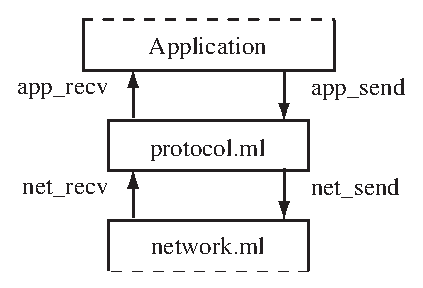
\includegraphics{network_stack}
\end{center}
%
With this design, the \hbox{\lstinline+Network+} component
calls \hbox{\lstinline+Protocol.net_recv+} when a message arrives, and
the \hbox{\lstinline+Protocol+} component
calls \hbox{\lstinline+Network.net_send+} to send a message.  However,
this is not possible if the implementations are in separate
files \hbox{\lstinline+protocol.ml+} and \hbox{\lstinline+network.ml+}
because that would introduce a cyclic dependency.

Describe a method to circumvent this problem, without placing the code
for the two components into a single file.

\begin{answer}\ifanswers
There are a few potential solutions, including the use of recursive
modules (discussed in Section~\ref{section:recursive-modules}) or
objects (Chapter~\ref{chapter:objects}).  In addition here are a few
alternate ways.

\begin{enumerate}
\item

If the design can be partitioned into two separate message streams
without any cycles, the design can be programmed directly.

\begin{center}
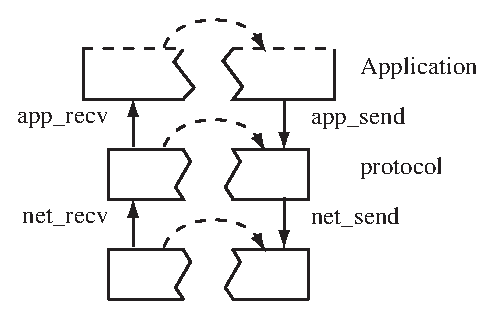
\includegraphics{network_stack2}
\end{center}
%
However, this approach may not be possible, and the changes required
may be unnatural.

\item

A simpler solution is to introduce a third file containing references
that can be set to refer each of the functions.  This solution, while
lacking elegance, is straightforward.

\begin{center}
\begin{tabular}{l}
refs.mli\\
\hline
\begin{minipage}{5in}
\begin{ocaml}
val net_recv_ref : (message -> unit) ref
val net_send_ref : (message -> unit) ref
val app_recv_ref : (message -> unit) ref
val app_send_ref : (message -> unit) ref
\end{ocaml}
\end{minipage}
\end{tabular}
\end{center}
%
The cells are initialized with dummy values.
\begin{ocaml}
let net_recv_ref = ref (fun _ -> raise (Invalid_argument "not initialized"))
...
\end{ocaml}
%
At startup time, the layers set the references to refer to the
appropriate functions.

\begin{center}
\begin{tabular}{l}
protocol.ml\\
\hline
\begin{minipage}{3in}
\begin{ocaml}
let net_recv msg = ...
...
Refs.net_recv_ref := net_recv
\end{ocaml}
\end{minipage}
\end{tabular}
\end{center}

\item

Yet another option is to define a third file,
say \hbox{\lstinline+link.ml+} that builds the recursive definition in
a single file.  Each of the layer functions would take as arguments
the functions that it expects to call.

\begin{ocaml}
let rec net_recv msg =
   Protocol.net_recv net_send app_recv msg
and app_send msg =
   Protocol.app_send net_send app_recv msg
and net_send msg =
   Network.net_send net_recv msg
and app_recv msg =
   Application.app_recv app_send msg
\end{ocaml}
%
This solution is more complicated and may be slightly less efficient
than the solution using reference cells.

\end{enumerate}
\fi\end{answer}
\end{exercise}

% -*-
% Local Variables:
% Mode: LaTeX
% fill-column: 100
% TeX-master: "paper"
% TeX-command-default: "LaTeX/dvips Interactive"
% End:
% -*-
% vim:tw=100:fo=tcq:

%
%
%

%%%%%%%%%%%%%%%%%%%%%%%%%%%%%%%%%%%%%%%%%%%%%%%%%%%%%%%%%%%%%%%%%%%%%%%%
% Exercises
%
\exercises

\begin{exercise}{struct1}
Which of the following are legal programs?  Explain your answers.
\begin{enumerate}
\item

\begin{ocamllisting}
module A : sig
   val x : string
end = struct
   let x = 1
   let x = "x"
end
\end{ocamllisting}

\item

\begin{ocamllisting}
module A : sig
   val x : string
   val x : string
end = struct
   let x = "x"
end
\end{ocamllisting}

\item

\begin{ocamllisting}
module a = struct
   let x = 1
end;;
\end{ocamllisting}

\item

\begin{ocamllisting}
module M : sig
   val f : int -> int
   val g : string -> string
end = struct
   let g x = x
   let f x = g x
end
\end{ocamllisting}

\item

\begin{ocamllisting}
let module X = struct let x = 1 end in X.x
\end{ocamllisting}

\item

\begin{ocamllisting}
module M = struct
   let g x = h x
   let f x = g x
   let h x = x + 1
end
\end{ocamllisting}

\item

\begin{ocamllisting}
module rec M : sig
   val f : int -> int
   val h : int -> int
end = struct
   open M
   let g x = h x
   let f x = g x
   let h x = x + 1
end
\end{ocamllisting}

\item

\begin{ocamllisting}
module rec M : sig
   val f : int -> int
end = struct
   let f = M.f
end
\end{ocamllisting}

\item

\begin{ocamllisting}
type 'a t = { set : 'a -> unit; get : unit -> 'a }
let f x =
   let cell = ref x in
   let module M = struct
      let s i = cell := i
      let g () = !cell
      let r = { set = s; get = g }
   end
   in
      M.r
\end{ocamllisting}

\item

\begin{ocamllisting}
let f x =
   let cell = ref x in
   let module M = struct
      type 'a t = { set : 'a -> unit; get : unit -> 'a }
      let s i = cell := i
      let g () = !cell
      let r = { set = s; get = g }
   end
   in
      M.r
\end{ocamllisting}

\item

\begin{ocamllisting}
module type ASig = sig type s  val f : int -> s end
module type BSig = sig type t  val g : t -> int end
module C : sig
   module A : ASig
   module B : BSig with type t = A.s
end = struct
   type u = string
   module A = struct type s = u  let f = string_of_int end
   module B = struct type t = u  let g = int_of_string end
end
include C
let i = B.g (A.f ())
\end{ocamllisting}   

\item

\begin{ocamllisting}
module type ASig = sig type t end
module type BSig = sig val x : int end
module A : ASig with type t = int
   = struct type t = int end
module B : BSig = struct let x = 1 end
module C : sig
   include ASig
   val x : t
end = struct
   include A
   include B
end
\end{ocamllisting}
\end{enumerate}

\begin{answer}\ifanswers
\begin{enumerate}
\item

Legal; the value associated with a variable is specified by the last
definition in the module.
\item 

Legal; the duplicate type definition is legal.  What would happen if
the type definitions differ?
\item 

Not legal; the module name must begin with an uppercase letter.
\item 

Legal; within the structure body the function \hbox{\lstinline/g/} has
type \hbox{\lstinline$'a -> 'a$}.  The type constraint is
applied \emph{after} the structure is formed.
\item 

Legal; the value is \hbox{\lstinline$1$}.
\item 

Not legal; the function \hbox{\lstinline/h/} must be defined before \hbox{\lstinline/g/}.
\item 

Legal; the forward reference to \hbox{\lstinline$h x$} is allowed
because the module is recursive.
\item 

Legal; however a application of the function \hbox{\lstinline/f/} will fail at
runtime because the value cannot be resolved.
\item 

Legal; \hbox{\lstinline/f/} has type \hbox{\lstinline$f : 'a -> 'a t$}.
\item

Not legal; OCaml produces the error message ``In this type, the
locally bound module name M escapes its scope.''  This is because the
the function \hbox{\lstinline/f/} produces a value of type \hbox{\lstinline$M.t$},
but \hbox{\lstinline$M$} is defined only in the body of \hbox{\lstinline/f/}.

\item

Legal; the modules \hbox{\lstinline/A/} and \hbox{\lstinline/B/} share a common (abstract) type,
so it is legal to pass the result of \lstinline $A.f$
t \hbox{\lstinline$B.g$}.

\item

Legal; the \hbox{\lstinline$include$} directive is like textual inclusion,
subject to signature constraints.  After expansion, the module \hbox{\lstinline/C/}
has the following form.

\begin{ocaml}
module C : sig
   type t
   val x : t
end = struct
   type t = int (* sig type t = int *)
   let x = 1    (* sig val x : int *)
end
\end{ocaml}
%
This is a legal module definition.
\end{enumerate}
\fi\end{answer}
\end{exercise}

%%%%%%%%%%%%%%%%%%%%%%%%%%%%%%%%%%%%%%%%%%%%%%%%%%%%%%%%%%%%%%%%%%%%%%%%
%
%
\begin{exercise}{struct1}
In OCaml, programs are usually written ``bottom-up,'' meaning that
programs are constructed piece-by-piece, and the last function is a
file is likely to be the most important.  Many programmers prefer a
top-down style, where the most important functions are defined first
in a file, and supporting definitions are placed later in the file.
Can you use the module system to allow top-down programming?

\begin{answer}\ifanswers
Recursive modules can be used for the top-down programming style.  The
code is wrapped in a module, and all forward references must be
declared in the module signature.  To illustrate, suppose we have a
function \hbox{\lstinline$main$} that calls
functions \hbox{\lstinline$f$} and \hbox{\lstinline$g$}, using an
intermediate type \hbox{\lstinline$t$}.

\begin{ocaml}
module rec Body : sig
   type t = V of int
   val main : int -> int
   val f : int -> t
   val g : t -> int
end = struct
   open Body

   let main i = g (f i)
   let f i = V i
   let g (V i) = i
   type t = V of int
end
\end{ocaml}
%
This approach has the usual disadvantage that types must be defined
twice, once in the signature and once in the structure.  However, the
type definition can be defined before the module.  This is common
style even in top-down programming.
\fi\end{answer}
\end{exercise}

%%%%%%%%%%%%%%%%%%%%%%%%%%%%%%%%%%%%%%%%%%%%%%%%%%%%%%%%%%%%%%%%%%%%%%%%
% 
%
\begin{exercise}{struct2}
One could argue that sharing constraints are never necessary for
unparameterized modules like the ones in this chapter. In the example
of Figure~\reffigure{xmset8}, there are at least two other solutions
that allow the \hbox{\lstinline/Set2/} and \hbox{\lstinline/Set/}
modules to share values, without having to use sharing
constraints. Present two alternate solutions without sharing
constraints.
\end{exercise}

\begin{exercise}{struct3}
In OCaml, signatures can apparently contain multiple declarations for the same value.

\begin{ocaml}
# module type ASig = sig
   val f : 'a -> 'a
   val f : int -> int
  end;;
@
\begin{topoutput}
module type ASig = sig val f : 'a -> 'a val f : int -> int end
\end{topoutput}
@
\end{ocaml}
%
In any structure that is given this signature, the
function \hbox{\lstinline$f$} must have \emph{all} the types listed.
If \hbox{\lstinline$f$} is not allowed to raise an exception, what is
the only sensible definition for it?

\begin{answer}\ifanswers
Instead of using a sharing constraint, we can add the type definition
directly in the signature.

\begin{ocaml}
module type Set2Sig = sig
   type 'a set = 'a Set.set
   val empty : 'a set
   ...
end
\end{ocaml}
%
In fact, we don't even need to define a separate type.

\begin{ocaml}
module type Set2Sig = sig
   val empty : 'a Set.set
   val add : 'a Set.set -> 'a -> 'a Set.set
   val mem : 'a -> 'a Set.set -> bool
end
\end{ocaml}
\fi\end{answer}
\end{exercise}

%%%%%%%%%%%%%%%%%%%%%%%%%%%%%%%%%%%%%%%%%%%%%%%%%%%%%%%%%%%%%%%%%%%%%%%%
% 
%
\begin{exercise}{struct4}
Unlike \hbox{\lstinline/val/} declarations, \hbox{\lstinline/type/}
declarations must have distinct names in any structure or signature.

\begin{ocaml}
# module type ASig = sig
     type t = int
     type t = bool
  end;;
@
\begin{toperror}
Multiple definition of the type name t.
Names must be unique in a given structure or signature.
\end{toperror}
@
\end{ocaml}
%
While this particular example may seem silly, the real problem is that
all modules included with \lstinline$include$ must have disjoint type
names.

\begin{ocaml}
# module type XSig = sig
     type t
     val x : t
  end;;
# module A : XSig = struct
     type t = int
     let x = 0
  end;;
# module B : XSig = struct
     type t = int
     let x = 1
  end;;
# module C = struct
     include A
     include B
  end;;
@
\begin{toperror}
Multiple definition of the type name t.
Names must be unique in a given structure or signature.
\end{toperror}
@
\end{ocaml}
%
Is this a problem?  If it is not, argue that conflicting includes
should not be allowed in practice.  If it is, propose a possible
solution to the problem (possibly by changing the language).

\begin{answer}\ifanswers
The type \hbox{\lstinline$'a -> 'a$} is more general than the
type \hbox{\lstinline$int -> int$}.  That is, any value with the
former type can also be given the latter type; the inverse does not
hold.  This means that the value must have
\hbox{\lstinline$'a -> 'a$}.
The only sensible value with this type is the identity function.

\begin{ocaml}
module A : ASig = struct
   let f x = x
end
\end{ocaml}
\end{answer}

\begin{answer}{struct4}
\fi\end{answer}
\end{exercise}

% -*-
% Local Variables:
% Mode: LaTeX
% fill-column: 100
% TeX-master: "paper"
% TeX-command-default: "LaTeX/dvips Interactive"
% End:
% -*-
% vim:tw=100:fo=tcq:

%
%
%
\exercises

%%%%%%%%%%%%%%%%%%%%%%%%%%%%%%%%%%%%%%%%%%%%%%%%%%%%%%%%%%%%%%%%%%%%%%%%
% Exercises
%
\begin{exercise}{functor1}
Which of the following are legal programs?  Explain your answers.

\begin{enumerate}
\item

\begin{ocamllisting}
module type XSig = sig val i : int end
module F (X : XSig) = X
\end{ocamllisting}

\item

\begin{ocamllisting}
module type S = sig end
module Apply (F : functor (A : S) -> S) (A : S) = F (A)
\end{ocamllisting}

\item

\begin{ocamllisting}
module type ISig = sig val i : int end
module F (I : ISig) : ISig = struct let i = I.i + 1 end
let j = F(struct let i = 1 end).i
\end{ocamllisting}

\item

\begin{ocamllisting}
module X = struct type t = int end
module F (X) = struct type t = X.t end
\end{ocamllisting}

\item

\begin{ocamllisting}
module F (X : sig type t = A | B end) : sig type t = A | B end = X
\end{ocamllisting}

\item

\begin{ocamllisting}
module F (X : sig type t = A | B end) : sig type t = A | B end =
struct type t = A | B end
\end{ocamllisting}

\item

\begin{ocamllisting}
module F (X : sig type t = A | B end) : sig type t = A | B end =
struct type t = X.t end
\end{ocamllisting}

\end{enumerate}

\begin{answer}\ifanswers
\begin{enumerate}
\item

Legal; the functor \hbox{\lstinline$F$} is the identity functor.
\item

Legal; the module expression \hbox{\lstinline$Apply (F) (A)$} is
equivalent to \hbox{\lstinline$F (A)$}.
\item

Not legal; the module expression
\hbox{\lstinline$F(struct let i = 1 end)$}
is not an expression.
\item

Not legal; the module parameter \hbox{\lstinline$X$} must have a
signature (as in $F (X : XSig)$).
\item

Legal; the module \hbox{\lstinline$X$} has the specified
signature \hbox{\lstinline$sig type t = A | B end$}.
\item

Legal; the structure \hbox{\lstinline$struct type t = A | B end$} has
signature \hbox{\lstinline$sig type t = A | B end$}.
\item

Not legal; the types \hbox{\lstinline$X.t$} and
\hbox{\lstinline$type t = X.t$}
are different types.
\end{enumerate}
\fi\end{answer}
\end{exercise}

%%%%%%%%%%%%%%%%%%%%%%%%%%%%%%%%%%%%%%%%%%%%%%%%%%%%%%%%%%%%%%%%%%%%%%%%
% 
%
\begin{exercise}{functor2}
Consider the following well-typed program.

\begin{ocaml}
module type T = sig type t val x : t end
module A = struct type t = int let x = 0 end
module B = struct type t = int let x = 0 end
module C = A
module F (X : T) = X
module G (X : T) : T = X
module D1 = F (A)
module D2 = F (B)
module D3 = F (C)
module E1 = G (A)
module E2 = G (B)
module E3 = G (C)
\end{ocaml}
%
Which of the following expressions are legal?  Which have type errors?

\begin{enumerate}
\item

\begin{ocamllisting}
D1.x + 1
\end{ocamllisting}

\item

\begin{ocamllisting}
D1.x = D2.x
\end{ocamllisting}

\item

\begin{ocamllisting}
D1.x = D3.x
\end{ocamllisting}

\item

\begin{ocamllisting}
E1.x + 1
\end{ocamllisting}

\item

\begin{ocamllisting}
E1.x = E2.x
\end{ocamllisting}

\item

\begin{ocamllisting}
E1.x = E3.x
\end{ocamllisting}

\item

\begin{ocamllisting}
D1.x = E1.x
\end{ocamllisting}
\end{enumerate}

\begin{answer}\ifanswers
The first three expressions are legal because, in each of
the \hbox{\lstinline$D$} modules, the type \hbox{\lstinline$t$}
is \hbox{\lstinline$int$}.  For the remaining four expressions, the
functor \hbox{\lstinline$G$} produces a module with
signature \hbox{\lstinline$T$}, where the type \hbox{\lstinline$t$} is
abstract.  In part 6, the expressions have types
%
\hbox{\lstinline$E1.x : G(A).t$} and \hbox{\lstinline$E3.x : G(C).x$}.
%
The types \hbox{\lstinline$G(A).t$} and $G(C).t$ are different, even
though modules \hbox{\lstinline$A$} and \hbox{\lstinline$C$} are
equal.
\fi\end{answer}
\end{exercise}

%%%%%%%%%%%%%%%%%%%%%%%%%%%%%%%%%%%%%%%%%%%%%%%%%%%%%%%%%%%%%%%%%%%%%%%%
%
%
\begin{exercise}{functor3}
How many lines of output does the following program produce?

\begin{ocaml}
module type S = sig val x : bool ref end

module F (A : S) =
struct
   let x = ref true;;
   if !A.x then begin
       print_string "A.x is true\n";
       A.x := false
   end
end

module G = F (F (F (struct let x = ref true end)))
\end{ocaml}

\begin{answer}\ifanswers
The body of a functor is not evaluated until the functor is applied.
Thus, the program prints one line of output for each functor
application (so there are three lines of output).
\fi\end{answer}
\end{exercise}

%%%%%%%%%%%%%%%%%%%%%%%%%%%%%%%%%%%%%%%%%%%%%%%%%%%%%%%%%%%%%%%%%%%%%%%%
%
%
\begin{exercise}{functor4}
\index{modules!vs records@\textit{vs.}~records}
It is sometimes better to define a data structure as a record instead
of a module.  For example, the record type for the finite sets in this
chapter might be defined as follows, where the
type \hbox{\lstinline$'elt t$} is the set representation for sets with
elements of type \hbox{\lstinline$'elt$}.

\begin{ocaml}
type 'elt t = $\cdots$
type 'elt set =
   { empty : 'elt t;
     add   : 'elt -> 'elt t -> 'elt t;
     mem   : 'elt -> 'elt t -> bool;
     find  : 'elt -> 'elt t -> 'elt
   }
\end{ocaml}
%
\begin{enumerate}
\item

Write a function
%
\hbox{\lstinline$make_set : ('elt -> 'elt -> bool) -> 'elt set$}
%
that corresponds to the \hbox{\lstinline$MakeSet$} functor on
page~\pageref{page:mset1} (the argument to \hbox{\lstinline$make_set$}
is the equality function).  Can you hide the definition of the type
%
\hbox{\lstinline$'elt t$}
%
from the rest of the program?

\item

Is it possible to implement sets two different ways such that both
implementations use the same \hbox{\lstinline$'elt set$} type, but
different \hbox{\lstinline$'elt t$} representations?

\item

Consider an alternative definition for sets, where the record type is
also parameterized by the set representation.

\begin{ocaml}
type ('elt, 't) set =
   { empty : 't;
     add   : 'elt -> 't -> 'elt;
     mem   : 'elt -> 't -> bool;
     find  : 'elt -> 't -> 'elt
   }
\end{ocaml}
%
Write the function \hbox{\lstinline$make_set$} for this new type.  What is
the type of the \hbox{\lstinline$make_set$} function?

\item

What are some advantages of using the record representation?  What are
some advantages of using the functor representation?
\end{enumerate}

\begin{answer}\ifanswers
\begin{enumerate}
\item

The definition is a direct translation of the
functor \hbox{\lstinline$MakeSet$}.

\begin{ocaml}
type 'elt t = 'elt list
let make_set equal =
   { empty = [];
     add = (::);
     mem = (fun x s -> List.mem (equal x) s);
     find = (fun x s -> List.find (equal x) s)
   }
\end{ocaml}
%
To keep the type \hbox{\lstinline$'elt t$} abstract, we must enclose the
definition in a module.

\begin{ocaml}
module Set : sig
   type 'elt t
   type 'elt set = $\cdots$
   val make_set : ('elt -> 'elt -> bool) -> 'elt set
end = struct
   type 'elt t = 'elt list
   type 'elt set = $\cdots$
   let make_set equal = $\cdots$
end
\end{ocaml}

\item

No.  The type \hbox{\lstinline$'elt t$} is fixed for all sets (of
type \hbox{\lstinline$'elt set$}).

\item

The implementation of the function \hbox{\lstinline$make_set$} is
unchanged.  It has the following type.

\begin{ocaml}
type 'elt set_repr = 'elt list
$\cdots$
val make_set : ('elt -> 'elt -> bool) -> ('elt, 'elt set_repr) set
\end{ocaml}
%
The type \hbox{\lstinline$set_repr$} is the representation for sets; the type
definition can be hidden the usual way.

\item

The main advantage of the record representation is that it
is \emph{first class}, meaning that values of
type \hbox{\lstinline$'elt set$} can be passed as arguments, stored in
data structures, etc.  There are several disadvantages.  Among them,
type expressions are larger.  In the worst case, the type definition
requires a parameter for each type that would be abstract in the
module.  In addition, there is a slight performance penalty for
calling a function in the \hbox{\lstinline$set$} record; the functor
does not have this penalty penalty because references are resolved at
compile time.

\end{enumerate}
\fi\end{answer}
\end{exercise}

%%%%%%%%%%%%%%%%%%%%%%%%%%%%%%%%%%%%%%%%%%%%%%%%%%%%%%%%%%%%%%%%%%%%%%%%
%
%
\begin{exercise}{functor5}
Suppose you wish to write a program that defines two
mutually-recursive functions \hbox{\lstinline$f : int -> int$}
and \hbox{\lstinline$g : int -> int$}.  To keep the design modular,
you wish to write the code for the two functions in separate
files \hbox{\lstinline$f.ml$} and \hbox{\lstinline$g.ml$}.  Describe
how to use recursive modules to accomplish the task.

\begin{answer}\ifanswers
Each function can be defined in its own file using a functor, where the
functor argument defines both functions.

\begin{ocaml}
module type RSig = sig
   val f : int -> int
   val g : int -> int
end

module FFun (R : RSig) = struct
   open R
   let rec f i = $\cdots$
end
\end{ocaml}
%
The glue code can be placed in a third file, using recursive modules
to ``tie the knot.''

\begin{ocaml}
module rec F : sig val f : int -> int end = FFun (R)
and F : sig val g : int -> int end = GFun (R)
and R : RSig = struct
   let f = F.f
   let g = G.g
end
\end{ocaml}
\fi\end{answer}
\end{exercise}

%%%%%%%%%%%%%%%%%%%%%%%%%%%%%%%%%%%%%%%%%%%%%%%%%%%%%%%%%%%%%%%%%%%%%%%%
%
%
\begin{exercise}{functor6}
\index{pipelines}
In Unix-style systems\footnote{UNIX\textregistered{} is a registered
trademark of The Open Group.} a \emph{pipeline} is a series of
processes \hbox{\lstinline/$p_1$ | $p_2$ | $\cdots$ | $p_n$/} that
interact through communication channels, where the input of process
$p_{i + 1}$ is the output of process $p_i$.

We can use a similar architecture within a program to connect modules,
which we will call \emph{filters}, giving them the
signature \hbox{\lstinline$Filter$}.  The pipeline itself is given the
signature \hbox{\lstinline$Pipeline$}, where the type of elements
passed into the pipeline have type \hbox{\lstinline$Pipeline.t$}.

\begin{ocaml}
module type Pipeline = sig
   type t
   val f : t -> unit
end

module type Filter = functor (P : Pipeline) -> Pipeline
\end{ocaml}
%
For example, the following pipeline \hbox{\lstinline$CatFile$}
prints the contents of a file to the terminal, one line at a time.

\begin{ocaml}
module Print = struct
   type t = string
   let f s = print_string s; print_char '\n'
end

module Cat (Stdout : Pipeline with type t = string) =
struct
   type t = string

   let f filename =
      let fin = open_in filename in
      try
         while true do Stdout.f (input_line fin) done
      with End_of_file -> close_in fin
end

module CatFile = Cat (Print)
\end{ocaml}

\begin{enumerate}
\item

Write a \hbox{\lstinline$Uniq$} filter that, given a sequence of input
lines, discards lines that are equal to their immediate predecessors.
All other lines should be passed to the output.

\item

Write a \hbox{\lstinline$Grep$} filter that, given a regular
expression and a sequence of input lines, outputs only those lines
that match the regular expression.  For regular expression matching,
you can use the \hbox{\lstinline$Str$} library.  The function
\hbox{\lstinline$Str.regexp : string -> regexp$}
compiles a regular expression presented as a string; the
expression \hbox{\lstinline$Str.string_match r s 0$} tests whether a
string $s$ matches a regular expression $r$.

\item

Write a function \hbox{\lstinline$grep : string -> string -> unit$},
where the expression \hbox{\lstinline$grep regex filename$} prints the
lines of the file \hbox{\lstinline/filename/} that match the pattern specified by
the string \hbox{\lstinline/regex/}, using the pipeline construction and the
module \hbox{\lstinline$Grep$} from the previous part.

\item

Sometimes it is more convenient for filters to operate over individual
characters instead of strings.  For example, the following filter
translates a character stream to lowercase.

\begin{ocaml}
module Lowercase (Stdout with type t = char) =
struct
   type t = char
   let f c = Stdout.f (Char.lowercase c)
end
\end{ocaml}
%
Write a filter \hbox{\lstinline$StringOfChar$} that converts a
character-based pipeline to a string-based pipeline.
%
\begin{ocaml}
StringOfChar : functor (P : Pipeline with type t = char) ->
   Pipeline with type t = string
\end{ocaml}

\item

The pipeline signatures, as defined, seem to require that pipelines be
constructed from the end toward the beginning, as a module expression
of the form \hbox{\lstinline/P1 (P2 $\cdots$ (Pn) $\cdots$)/}.  Write
a functor \hbox{\lstinline$Compose$} that takes two filters and
produces a new one that passes the output of the first to the second.
What is the signature of the \hbox{\lstinline$Compose$} functor?
(Hint: consider redefining the signature for filters.)
\end{enumerate}

\begin{answer}\ifanswers
\begin{enumerate}
\item

For the \hbox{\lstinline$Uniq$} filter, we can use a reference cell to
keep track of lines as they are read.  We ``cheat'' in this
solution---since we know the input never contains a newline, we
initialize the \misspelled{refcell} to an impossible value.  A better solution
would be for the cell to be initialized to \hbox{\lstinline$None$}
(and thus be of type \hbox{\lstinline$string option$}).

\begin{ocaml}
module Uniq (Stdout : Pipeline with type t = string)
 : Pipeline with type t = string =
struct
   type t = string
   let last_line = ref "\n"
   let f s =
      if s <> !last_line then
         Stdout.f s;
      last_line := s
end
\end{ocaml}

\item

The main problem in defining the \hbox{\lstinline$Grep$} filter is
that it takes a regular expression as an argument.  It is possible to
pass the regular expression in its own module, but this will mean that
the \hbox{\lstinline$Grep$} module works for only one regular
expression.  (The next part illustrates another solution to this
problem.)

\begin{ocaml}
module Grep
 (R : sig val regex : string end)
 (P : Pipeline with type t = string) =
struct
   type t = string
   let regexp = Str.regexp R.regex
   let f s =
      if Str.string_match regexp s 0 then
         P.f s
end
\end{ocaml}

\item

One easy way to define the \hbox{\lstinline$grep$} function is to use
a \hbox{\lstinline$let module$} construction to define the pipeline
within the function body.

\begin{ocaml}
let grep regex filename =
   let module P = Cat (Grep (struct let regex = regex end) (Print)) in
   P.f filename
\end{ocaml}

\item

The \hbox{\lstinline$StringOfChar$} module simply iterates through each
character of the input string.

\begin{ocaml}
module StringOfChar (P : Pipeline with type t = char)
 : Pipeline with type t = string =
struct
   type t = string
   let f s = String.iter P.f s
end
\end{ocaml}

\item

The \hbox{\lstinline$Compose$} functor takes three arguments, the
first filter \hbox{\lstinline$F1$}, the second
filter \hbox{\lstinline$F2$}, and the rest of the
pipeline \hbox{\lstinline$P3$}, where 
\hbox{\lstinline$Compose (F1) (F2) (P3) = F1 (F2 (P3))$}.
Thus, a partial application \hbox{\lstinline$Compose (F1) (F2)$} will
yield a filter.

The main issue with constructing the filter is with the constraints
about compatibility of the filters' types.  These sharing constraints
are not obvious.  Suppose filter \hbox{\lstinline$F1$} takes values of
type $t_1$, filter \hbox{\lstinline$F2$} takes values of type $t_2$,
and the rest of the pipeline \hbox{\lstinline$P3$} takes values of
type $t_3$.  For illustration, we would have the following
constraints.

\begin{ocaml}
module Compose
 (F1 : (P : Pipeline with type t = $t_2$) -> Pipeline with type t = $t_1$)
 (F2 : (P : Pipeline with type t = $t_3$) -> Pipeline with type t = $t_2$)
 (P3 : Pipeline with type t = $t_3$) = F1 (F2 (P3))
\end{ocaml}
%
The proper types are then as follows $t_3
= \hbox{\hbox{\lstinline/P3.t/}}$, $t_2
= \hbox{\lstinline{F2(P3).t}}$, and $t_1
= \hbox{\lstinline{F1(F2(P3)).t}}$.  However, using these definitions
directly is not possible because it would create forward references in
the type definition.  For example, the signature
for \hbox{\lstinline$F1$} would refer forward to the
modules \hbox{\lstinline$F2$} and \hbox{\lstinline$P3$}.  We could
reorder the arguments to eliminate the forward references, but then
the partial application would not work as we wish.

Arguably, the best solution is to redefine the signature for filters so
that they specify the types for both input and output.

\begin{ocaml}
module type Filter = sig
   type t_in
   type t_out
   module F : functor (P : Pipeline with type t = t_out) ->
      Pipeline with type t = t_in
end
\end{ocaml}
%
The filters themselves are not much different.  For example, here is
the filter \hbox{\lstinline$StringOfChar$}.

\begin{ocaml}
module StringOfChar
 : Filter with type t_in = string and type t_out = char =
struct
   type t_in = string
   type t_out = char
   module F (X : Pipeline with type t = char) = struct
      type t = string
      let f s = String.iter X.f s
   end
end
\end{ocaml}
%
The sharing constraints for the \hbox{\lstinline$Compose$} functor are
now easy to express.

\begin{ocaml}
module Compose
 (F1 : Filter)
 (F2 : Filter with type t_in = F1.t_out)
 : Filter with type t_in = F1.t_in and type t_out = F2.t_out =
struct
   type t_in = F1.t_in
   type t_out = F2.t_out
   module F (P3 : Pipeline with type t = t_out) = struct
      module Pipe = F1.F (F2.F (P3))
      type t = t_in
      let f = Pipe.f
   end
end
\end{ocaml}
%
The signature can be represented as follows.

\begin{ocaml}
Compose : functor (F1 : Filter) ->
  functor (F2 : Filter with type t_in = F1.t_out) ->
  Filter with type t_in = F1.t_in and type t_out = F2.t_out
\end{ocaml}
\end{enumerate}
\fi\end{answer}
\end{exercise}

% -*-
% Local Variables:
% Mode: LaTeX
% fill-column: 100
% TeX-master: "paper"
% TeX-command-default: "LaTeX/dvips Interactive"
% End:
% -*-
% vim:tw=100:fo=tcq:

\exercises

%%%%%%%%%%%%%%%%%%%%%%%%%%%%%%%%%%%%%%%%%%%%%%%%%%%%%%%%%%%%%%%%%%%%%%%%
% Constructor methods
%
\begin{exercise}{object1}
In Section~\ref{section:objects-functional-update} we implemented the three factory
functions \hbox{\lstinline/new_scale/}, \hbox{\lstinline/new_rotate/}, and \hbox{\lstinline/new_translate/} as methods,
claiming that it would avoid code duplication.  Write one of the factory functions as a normal
function (not a method).  How can you avoid code duplication?

\begin{answer}\ifanswers
Let's implement \hbox{\lstinline/new_scale/} as a normal function.

\begin{ocaml}
let new_scale sx sy =
   object
      val matrix = (sx, 0., 0., sy, 0., 0.)
      method transform (x, y) = $\cdots$
      method multiply matrix2 = $\cdots$
   end;;
\end{ocaml}
%
If the other functions were implemented the same way, the code for the methods \hbox{\lstinline/transform/}
and \hbox{\lstinline/multiply/} would be duplicated.  We can avoid this by creating a generic constructor
function that takes the entire matrix as an argument.

\begin{ocaml}
let new_transform matrix =
   object
      val matrix = matrix
      method transform (x, y) = $\cdots$
      method multiply matrix2 = $\cdots$
   end

let new_scale sx sy = new_matrix (sx, 0., 0., sy, 0., 0.)
let new_translate dx dy = new_matrix (1., 0., dx, 0., 1., dy)
let new_rotate theta =
   let s, c = sin theta, cos theta in
   new_transform (c, -.s, 0., s, c, 0.)
\end{ocaml}
\fi\end{answer}
\end{exercise}

%%%%%%%%%%%%%%%%%%%%%%%%%%%%%%%%%%%%%%%%%%%%%%%%%%%%%%%%%%%%%%%%%%%%%%%%
% Silly field definitions
%
\begin{exercise}{object2}
In Section~\ref{section:objects-factories} the factory functions include some apparently silly field
definitions.  For example, the function \hbox{\lstinline/new_poly/} includes the field
\hbox{\lstinline/val vertices = vertices/}.
What is the purpose of the field definition?  What would happen if it were
omitted?

\begin{answer}\ifanswers
The purpose of the code is to allow the functional update
\hbox{\lstinline/{< vertices = Array.map matrix#transform vertices >}/};
for this to work, \hbox{\lstinline/vertices/} must be a field of the object.
If the field definition were omitted, the functional update would fail.
\fi\end{answer}
\end{exercise}

%%%%%%%%%%%%%%%%%%%%%%%%%%%%%%%%%%%%%%%%%%%%%%%%%%%%%%%%%%%%%%%%%%%%%%%%
% Uniqueness
%
\begin{exercise}{object4}
Suppose we wish to enforce the fact that a program contains only one copy of an object.  For
example, the object may be an accounting object, and we wish to make sure the object is never copied
or forged.

The standard library module \hbox{\lstinline/Oo/} contains a function that copies any object.

\begin{ocaml}
   val copy : (< .. > as 'a) -> 'a
\end{ocaml}
%
Modify the following object so that it refuses to work after being copied.

\begin{ocaml}
let my_account =
object
   val mutable balance = 100
   method withdraw =
      if balance = 0 then
         raise (Failure "account is empty");
      balance <- balance - 1
end
\end{ocaml}

\begin{answer}\ifanswers
  The object is initially created with a reference \lstinline/self1/ to itself, using the \lstinline/self/ parameter,
  and the value of \lstinline/self/ is checked (with pointer equality) before the withdraw operation
  is allowed.  The value for \lstinline/self1/ has to be set in an initializer (when the value of \lstinline/self/ is known).
  For simplicity, we use the empty object \lstinline/object end/ for the initial value of \lstinline/self1/.
\begin{ocaml}
let my_account =
object (self : 'self)
    val mutable balance = 100
    val mutable self1 : < > = object end
    initializer self1 <- (self :> < >)
    method withdraw =
        if (self :> < >) != self1 then
           raise (Failure "object has been copied");
        if balance = 0 then
           raise (Failure "account is empty");
        balance <- balance - 1
end
\end{ocaml}
\fi\end{answer}
\end{exercise}

%%%%%%%%%%%%%%%%%%%%%%%%%%%%%%%%%%%%%%%%%%%%%%%%%%%%%%%%%%%%%%%%%%%%%%%%
% Subtyping
%
\begin{exercise}{classes-subtype1}
For each of the following instances of types $t_1$ and $t_2$,
determine whether $t_1$ is a subtype of $t_2$---that is, whether $t_1 \subtype t_2$.
Assume the following class declarations and relations.

\begin{center}
\begin{tabular}{|l|}
\hline
Subtyping relations\\
\hline
\hbox{\lstinline/dog $\subtype$ animal/}\\
\hbox{\lstinline/cat $\subtype$ animal/}\\
\hline
\end{tabular}
\end{center}

\begin{enumerate}
\item

\begin{ocamllisting}
type $t_1$ = animal -> cat
type $t_2$ = dog -> animal
\end{ocamllisting}

\item

\begin{ocamllisting}
type $t_1$ = animal ref
type $t_2$ = cat ref
\end{ocamllisting}

\item

\begin{ocamllisting}
type 'a cl = < f : 'a -> 'a >
type $t_1$ = dog cl
type $t_2$ = animal cl
\end{ocamllisting}

\item

\begin{ocamllisting}
type 'a cl = < x : 'a ref >
type $t_1$ = dog cl
type $t_2$ = animal cl
\end{ocamllisting}

\item

\begin{ocamllisting}
type 'a c1 = < f : 'a -> unit; g : unit -> 'a >
type 'a c2 = < f : 'a -> unit >
type $t_1$ = animal c1
type $t_2$ = cat c2
\end{ocamllisting}

\item

\begin{ocamllisting}
type $t_1$ = ((animal -> animal) -> animal) -> animal
type $t_2$ = ((cat -> animal) -> dog) -> animal
\end{ocamllisting}

\end{enumerate}

\begin{answer}\ifanswers
\begin{enumerate}
\item $t_1 \subtype t_2$, because \hbox{\lstinline/dog $\subtype$ animal/} and \hbox{\lstinline/cat $\subtype$ animal/}.
\item $t_1 \not\subtype t_2$, because \hbox{\lstinline$'a refcell$} is invariant in \hbox{\lstinline$'a$}.
\item $t_1 \not\subtype t_2$, the class \hbox{\lstinline$'a cl$} is invariant in \hbox{\lstinline$'a$}.
\item $t_1 \not\subtype t_2$, because \hbox{\lstinline$'a refcell$} is invariant in \hbox{\lstinline$'a$}.
\item $t_1 \subtype t_2$, because \hbox{\lstinline$'a c2$} is contravariant in \hbox{\lstinline$'a$}.
\item $t_1 \subtype t_2$, because the type \hbox{\lstinline$(('a -> animal) -> 'b) -> animal$}
is contravariant in \hbox{\lstinline$'a$} and \hbox{\lstinline$'b$}.
\end{enumerate}
\fi\end{answer}
\end{exercise}

%%%%%%%%%%%%%%%%%%%%%%%%%%%%%%%%%%%%%%%%%%%%%%%%%%%%%%%%%%%%%%%%%%%%%%%%
% Narrowing
%
\begin{exercise}{narrowing-with-polymorphic-variants}
Let's reimplement the narrowing example from page~\pageref{page:narrowing-with-exceptions} in terms of
polymorphic variants instead of exceptions.  The type definitions can be given as follows.

\begin{ocaml}
type 'a animal = < actual : 'a; eat : unit >
type 'a dog = < actual : 'a; eat : unit; bark : unit >
type 'a cat = < actual : 'a; eat : unit; meow : unit >

type 'a tag = [> `Dog of 'a tag dog | `Cat of 'a tag cat ] as 'a
\end{ocaml}
%
\begin{enumerate}
\item Implement the rest of the example, including the function \hbox{\lstinline/chorus/}.
\item What does the type variable \hbox{\lstinline/'a/} represent?
\item What must be changed when a new type of animals is added, say \hbox{\lstinline/'a lizard/},
for lizards that eat but don't vocalize?
\end{enumerate}

\begin{answer}\ifanswers
\begin{enumerate}
\item
The complete solution is mainly unchanged from the code that uses exceptions.

\begin{ocaml}
type 'a animal = < actual : 'a; eat : unit >
type 'a dog = < actual : 'a; eat : unit; bark : unit >
type 'a cat = < actual : 'a; eat : unit; meow : unit >

type 'a tag = [> `Dog of 'a tag dog | `Cat of 'a tag cat ] as 'a

let fido : 'a tag dog =
object (self)
   method actual = `Dog self
   method eat = ()
   method bark = ()
end;;

let daphne : 'a tag cat =
object (self)
   method actual = `Cat self
   method eat = ()
   method meow = ()
end;;

let animals = [(fido :> 'a tag animal); (daphne :> 'a tag animal)];;

let chorus (animals : 'a tag animal list) =
   List.iter (fun animal ->
      match animal#actual with
         `Dog dog -> dog#bark
       | `Cat cat -> cat#meow
       | _ -> ()) animals
\end{ocaml}

\item The type variable \hbox{\lstinline/'a/} stands for the real type of tags.
The tag type contains at least the tags \hbox{\lstinline/`Dog/} and \hbox{\lstinline/`Cat/}, but it is an open
type, so the actual type \hbox{\lstinline/'a/} may contain additional constructors.

\item Since lizards don't vocalize, we really don't need to change any of the existing
code.  We simple add the new object with a new tag.

\begin{ocaml}
let fred : 'a tag lizard =
object (self)
   method actual = `Lizard self
   method eat = ()
end;;
\end{ocaml}
\end{enumerate}
\fi\end{answer}
\end{exercise}

\begin{exercise}{narrowing2}
The narrowing technique on page~\pageref{page:narrowing-with-exceptions} skirts an important
problem---what if the inheritance hierarchy has multiple levels?  For example, we might have the
following relationships.

\begin{ocaml}
hound $\subtype$ dog $\subtype$ animal
tabby $\subtype$ cat $\subtype$ animal
\end{ocaml}
%
In a \misspelled{na\"\i{}ve} implementation, typecases would have to be updated whenever a new tag is added.  For example, the
\hbox{\lstinline/chorus/} function might require at least four cases.

\begin{ocaml}
let chorus (animals : animal list) =
   List.iter (fun animal ->
      match animal#actual with
         Dog dog -> dog#bark
       | Hound hound -> hound#bark
       | Cat cat -> cat#meow
       | Tabby tabby -> tabby#meow
       | _ -> ()) animals
\end{ocaml}
%
This is undesirable of course, since the \hbox{\lstinline/chorus/} function cares only about the general
cases \hbox{\lstinline/dog/} and \hbox{\lstinline/cat/}.

Modify the implementation so that the method \hbox{\lstinline/actual/} takes a list of acceptable tags as
an argument.  For example, for a hound \hbox{\lstinline/hound/}, the expression
\hbox{\lstinline/hound#actual [CatTag; DogTag]/} would evaluate to \hbox{\lstinline/Dog hound/};
but \hbox{\lstinline/hound#actual [HoundTag; DogTag; CatTag]/} would evaluate to \hbox{\lstinline/Hound hound/}.

\begin{answer}\ifanswers
To keep it simple, we'll use exceptions both as tags and actual values.

\begin{ocaml}
type actual = exn list -> exn
type animal = < actual : actual; eat : unit >
type dog = < actual : actual; eat : unit; bark : unit >
type cat = < actual : actual; eat : unit; meow : unit >
type hound = < actual : actual; eat : unit; bark : unit; howl : unit >

exception DogTag
exception CatTag
exception HoundTag

exception Dog of dog
exception Cat of cat
exception Hound of hound

let fido : hound =
object (self)
   method actual tags =
      match tags with
         HoundTag :: _ -> Hound self
       | DogTag :: _ -> Dog (self :> dog)
       | _ :: tags -> self#actual tags
       | [] -> Not_found
   method eat = ()
   method bark = ()
   method howl = ()
end;;

let chorus (animals : animal list) =
   List.iter (fun animal ->
      match animal#actual [DogTag; CatTag] with
         Dog dog -> dog#bark
       | Cat cat -> cat#meow
       | _ -> ()) animals
\end{ocaml}
\fi\end{answer}
\end{exercise}

%%%%%%%%%%%%%%%%%%%%%%%%%%%%%%%%%%%%%%%%%%%%%%%%%%%%%%%%%%%%%%%%%%%%%%%%
% Representation
%
\begin{exercise}{objects-implementation}
In OCaml, an object of type $t_1$ can be coerced to any supertype $t_2$, regardless of whether type $t_2$
has a name.  This differs from some other languages.  For example, in C++, an object can safely be
coerced to any of its superclasses, but arbitrary supertypes are not allowed.  This is mainly
because objects in C++ are represented as a sequence of fields and methods (for space efficiency, methods
are usually represented in a separate array called a \misspelled{\emph{vtable}}).  For instance, if class $C$ is
a subclass of two independent classes $A$ and $B$, their representations are laid out in order.

\begin{center}
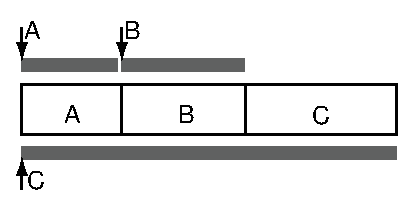
\includegraphics[scale=0.75]{c++-object}
\end{center}
%
The object $A$ is laid out first, followed by $B$, then any additional fields in $C$.  A pointer to
a $C$ object is also a pointer to an $A$, so this coercion has no runtime cost.  The coercion from
$C$ to $B$ is also allowed with a bit of pointer arithmetic.

In OCaml, the situation is quite different.  The order of methods and fields in an object doesn't
matter, coercions to arbitrary supertypes are allowed, and coercions never have a runtime cost.  To
help understand how this works, let's build a model of objects using polymorphic variants.

Abstractly, an object is just a thing that reacts to messages that are sent to it---in other words,
it is a function on method names.  Given an object $o$ with method names $m_1, m_2, \ldots, m_n$, the
names are given variant labels \hbox{\lstinline/`L_m1/}, \hbox{\lstinline/`L_m2/}, $\ldots$, \hbox{\lstinline/`L_mn/}.  The
object becomes a pattern match over method labels, and the fields become let-definitions.
Here is a dog object together with the corresponding model.

\begin{center}
\begin{tabular}{c|c}
Object & Model\\
\hline
\begin{minipage}[t]{2.2in}
\begin{ocamllisting}
type dog =
   < eat : unit;
     bark : unit;
     chase : string -> unit
   >

let dog s =
object (self)
   val name = s
   method eat = printf "%s eats\n" name
   method bark = printf "%s barks\n" name
   method chase s =
      self#bark;
      printf "%s chases %s\n" name s
end
\end{ocamllisting}
\end{minipage}
&
\begin{minipage}[t]{2.2in}
\begin{ocamllisting}
! type model_dog =
!    l:[`L_eat | `L_bark | `L_chase] -> 
!       (match l with
!           `L_eat | `L_bark -> unit
!         | `L_chase -> (string -> unit))

let model_dog s =
   let name = s in
   let rec self = function
      `L_eat -> printf "%s eats\n" name
    | `L_bark -> printf "%s barks\n" name
    | `L_chase -> (fun s ->
          self `L_bark;
          printf "%s chases %s\n" name s)
   in
   self
\end{ocamllisting}
\end{minipage}
\end{tabular}
\end{center}
%
The recursive function \hbox{\lstinline/self/} represents the object.  It takes a method label, and returns
the method value.  The type \hbox{\lstinline/model_dog/} can't be defined in OCaml, because it is
a \emph{dependent} type.  Informally it says that a \hbox{\lstinline/model_dog/} is a function that takes a
label \hbox{\lstinline/l/}.  If \hbox{\lstinline/l/} is \hbox{\lstinline/`L_eat/} or \hbox{\lstinline/`L_bark/}, then the result
type is \hbox{\lstinline/unit/}.  If the label is \hbox{\lstinline/`L_chase/}, the result type
is \hbox{\lstinline/string -> unit/}.

\begin{enumerate}
\item Suppose an animal object is defined as follows.

\begin{ocaml}
type animal = < eat : unit >
let animal s = object method eat = printf "%s eats\n" s end
\end{ocaml}
%
Write the model \hbox{\lstinline/model_animal/} for an animal object.

\item
Given a \hbox{\lstinline/model_dog/} $e$, how is a coercion \hbox{\lstinline/($e$ : model_dog :> model_animal)/} implemented?

\item
How is a coercion \hbox{\lstinline/($e$ : dog :> < chase : string -> unit >)/} implemented in the model?
\end{enumerate}
%
Suppose that, instead of representing fields as individual let-definitions, the fields of an object
are collected in a record, with the compiler inserting the appropriate projections.  For example,
here is a revised \hbox{\lstinline/model_dog/}.

\begin{ocaml}
type dog_fields = { name : string }

let model_dog s =
   let rec self fields = function
      `L_eat -> printf "%s eats\n" fields.name
    | `L_bark -> printf "%s barks\n" fields.name
    | `L_chase -> (fun s ->
          self fields `L_bark;
          printf "%s chases %s\n" fields.name s)
   in
   self { name = s }
\end{ocaml}
%
\begin{enumerate}
\item[4.] In this revised version, how is a functional update implemented?
Explain your answer by giving the model for a new method

\begin{ocaml}
method new_dog s = {< name = s >}.
\end{ocaml}

\item[5.]
What is the complexity of method dispatch?  Meaning, given an arbitrary method label, how long does
it take to perform the pattern match?
\end{enumerate}
%
Suppose the pattern match is hoisted out of the object into a separate function \hbox{\lstinline/vtable/}.

\begin{ocaml}
let model_dog s =
   let vtable = function
      `L_eat -> (fun self fields -> printf "%s eats\n" fields.name)
    | `L_bark -> (fun self fields -> printf "%s barks\n" fields.name)
    | `L_chase -> (fun self fields s ->
          self fields `L_bark;
          printf "%s chases %s\n" fields.name s)
   in
   let rec self fields label =
      vtable label self fields
   in
   self { name = s }
\end{ocaml}
%
\begin{enumerate}
\item[6.]  What are the advantages of the separate \hbox{\lstinline/vtable/}?  What are some disadvantages?
\end{enumerate}

\begin{answer}\ifanswers
\begin{enumerate}
\item 

\begin{ocaml}
let animal_model s =
   let rec self = function
      `L_eat -> printf "%s eats\n" s
   in
   self
\end{ocaml}

\item

A \hbox{\lstinline/model_dog/} has all the methods of a \hbox{\lstinline/model_animal/} so it can be used as an
animal unchanged.  The coercion returns the dog without change.  To be more precise, consider the
types.

\begin{ocaml}
type model_dog = l:[`L_eat | `L_bark | `L_chase] -> $\cdots$
type model_animal = l:[`L_eat] -> $\cdots$
\end{ocaml}
%
The relation \hbox{\lstinline/model_dog $\subtype$ model_animal/} holds because
\hbox{\lstinline/[`L_eat] $\subtype$ [`L_eat | `L_bark | `L_chase]/}.

\item 

A \hbox{\lstinline/model_dog/} can be used as a model-\hbox{\lstinline/< chase : string -> unit>/} without change.

\item

A functional update becomes a record update.
The new method \hbox{\lstinline/new_dog/} is modeled as follows.

\begin{ocaml}
let model_dog s =
   let rec self fields = function
      $\cdots$
    | `L_new_dog s ->
        self { fields with name = s }
   in
   self { name = s }
\end{ocaml}

\item

The pattern match is really just a table lookup, so it can be implemented in $O(\log n)$ time, where
$n$ is the number of labels.  However, the number of labels in the program is fixed, so the pattern
match can be implemented in constant time.

\item

The advantage of hoisting the \hbox{\lstinline/vtable/} is that it can be shared by multiple dog objects.
The disadvantage is that it may be slightly more expensive because of the extra function call.
\end{enumerate}
\fi\end{answer}      
\end{exercise}

% -*-
% Local Variables:
% Mode: LaTeX
% fill-column: 100
% TeX-master: "paper"
% TeX-command-default: "LaTeX/dvips Interactive"
% End:
% -*-
% vim:tw=100:fo=tcq:

\exercises

%%%%%%%%%%%%%%%%%%%%%%%%%%%%%%%%%%%%%%%%%%%%%%%%%%%%%%%%%%%%%%%%%%%%%%%%
% Class types
%
\begin{exercise}{class-types1}
What are the class types for the following classes?

\begin{enumerate}
\item

\begin{ocamllisting}
class c1 =
object
   val x = 1
   method get = x
end
\end{ocamllisting}

\begin{answer}\ifanswers
\begin{ocamllisting}
class c1 :
object
   val x : int
   method get : int
end
\end{ocamllisting}
\fi\end{answer}

\item

\begin{ocamllisting}
class c2 =
object
   method copy = {< >}
end
\end{ocamllisting}

\begin{answer}\ifanswers
\begin{ocamllisting}
class c2 :
object ('self)
   method copy : 'self
end
\end{ocamllisting}
\fi\end{answer}

\item

\begin{ocamllisting}
class c3 y =
object (self1)
   method f x =
      object (self2)
         val x = x
         method h = self1#g + x
      end
   method g = y
end
\end{ocamllisting}

\begin{answer}\ifanswers
\begin{ocamllisting}
class c3 : int ->
object
   method f : int -> < h : int >
   method g : int
end
\end{ocamllisting}
\fi\end{answer}

\item

\begin{ocamllisting}
class c4 =
object (self : < x : int; .. > as 'self)
   method private x = 1
end
\end{ocamllisting}

\begin{answer}\ifanswers
The type constraint removes the private status of the method \hbox{\lstinline/x/}.
\begin{ocamllisting}
class c4 :
object 
   method x : int
end
\end{ocamllisting}
\fi\end{answer}
\end{enumerate}
\end{exercise}

%%%%%%%%%%%%%%%%%%%%%%%%%%%%%%%%%%%%%%%%%%%%%%%%%%%%%%%%%%%%%%%%%%%%%%%%
% Initializer order
%
\begin{exercise}{classes-initializer-order}
What does the following program print out?

\begin{ocaml}
class a (i : int) =
let () = print_string "A let\n" in
object
   initializer print_string "A init\n"
end;;

class b (i : int) =
let () = print_string "B let\n" in
object
   inherit a i
   initializer print_string "B init\n"
end;;

new b 0;;
\end{ocaml}

\begin{answer}\ifanswers
The order of the let-expressions and initializers follows the textual order.
Class \hbox{\lstinline/a/} is nested within \hbox{\lstinline/b/}, but before \hbox{\lstinline/b/}'s initializer.
The sequence is the following.

\begin{ocaml}
B let
A let
A init
B init
\end{ocaml}
\fi\end{answer}
\end{exercise}

%%%%%%%%%%%%%%%%%%%%%%%%%%%%%%%%%%%%%%%%%%%%%%%%%%%%%%%%%%%%%%%%%%%%%%%%
% Inverted inheritance
%
\begin{exercise}{classes1}
Normally, we would consider a square to be a subtype of rectangle.
Consider the following class \hbox{\lstinline/square/} that implements a square,

\begin{ocaml}
class square x y w =
object
   val x = x
   val y = y
   method area = w * w
   method draw = Graphics.fill_rect x y w w
   method move dx dy = {< x = x + dx; y = y + dy >}
end
\end{ocaml}
%
Write a class \hbox{\lstinline/rectangle/} that implements a rectangle by inheriting from \hbox{\lstinline/square/}.
Is it appropriate to say that a \hbox{\lstinline/rectangle/} is a \hbox{\lstinline/square/}?

\begin{answer}\ifanswers
The class \hbox{\lstinline/rectangle/} adds a new dimension \hbox{\lstinline/h/}.
\begin{ocaml}
class rectangle x y w h =
object
   inherit square
   method area = w * h
   method draw = Graphics.fill_rect x y w h
end
\end{ocaml}
%
It is appropriate to say that the \emph{representation} of a rectangle includes the representation
of a square.  The is-a relationships in the program are defined by the programmer.  They don't have
to correspond to real-life relationships.
\fi\end{answer}
\end{exercise}

%%%%%%%%%%%%%%%%%%%%%%%%%%%%%%%%%%%%%%%%%%%%%%%%%%%%%%%%%%%%%%%%%%%%%%%%
% Lists
%
\begin{exercise}{classes-lists}
A mutable list of integers can be represented in object-oriented form with the following class type.

\begin{ocaml}
class type int_list =
object
    method is_nil : bool
    method hd : int
    method tl : int_list
    method set_hd : int -> unit
    method set_tl : int_list -> unit
end
\end{ocaml}
%
\begin{enumerate}
\item
Define classes \hbox{\lstinline/nil/} and \hbox{\lstinline/cons/} that implement the usual list constructors.

\begin{ocaml}
class nil : int_list
class cons : int -> int_list -> int_list
\end{ocaml}

\begin{answer}\ifanswers
The class \hbox{\lstinline/nil/} returns \hbox{\lstinline/true/} for the method \hbox{\lstinline/is_nil/},
and it raises an exception on all other operations.

\begin{ocaml}
class nil : int_list =
object (_ : #int_list as 'self)
   method is_nil = true
   method hd = raise (Invalid_argument "hd")
   method tl = raise (Invalid_argument "tl")
   method set_hd _ = raise (Invalid_argument "set_hd")
   method set_tl _ = raise (Invalid_argument "set_tl")
end
\end{ocaml}
%
The class \hbox{\lstinline/cons/} implements the mutable cons-cell.
The constraint \hbox{\lstinline/_ : #int_list as 'self/} is used to simplify
the types.

\begin{ocaml}
class cons hd tl =
object (_ : #int_list as 'self)
   val mutable hd = hd
   val mutable tl = tl
   method is_nil = false
   method hd = hd
   method tl = tl
   method set_hd x = hd <- x
   method set_tl l = tl <- l
end
\end{ocaml}
\fi\end{answer}

\item

The class type \hbox{\lstinline/int_list/} is a recursive type.  Can it be generalized to the following type?

\begin{ocaml}
class type gen_int_list =
object ('self)
    method is_nil : bool
    method hd : int
    method tl : 'self
    method set_hd : int -> unit
    method set_tl : 'self -> unit
end
\end{ocaml}

\begin{answer}\ifanswers
No, it is not possible to generalize the type, at least not easily.
The problem is that the class \hbox{\lstinline/cons/} takes the \hbox{\lstinline/tl/} as an argument.
If we try to implement it, we get the error ``Self type cannot escape its class,''
because the argument \hbox{\lstinline/tl/} has the same type as the class being defined.

\begin{ocaml}
class cons hd tl =
object (_ : #gen_int_list as 'self)
$\cdots$
end
@
\begin{topoutput}
      This expression has type 'a but is here used with type
        < hd : int; is_nil : bool; set_hd : int -> unit; set_tl : 'b -> unit;
          tl : 'b; .. >
        as 'b
      Self type cannot escape its class
\end{topoutput}
@
\end{ocaml}
\fi\end{answer}

\item

The class type \hbox{\lstinline/int_list/} should also include the usual list functions.

\begin{ocaml}
class type int_list =
object
    method is_nil : bool
    method hd : int
    method tl : int_list
    method set_hd : int -> unit
    method set_tl : int_list -> unit
    method iter : (int -> unit) -> unit
    method map  : (int -> int) -> int_list
    method fold : 'a. ('a -> int -> 'a) -> 'a -> 'a
end
\end{ocaml}
%
Implement the methods \hbox{\lstinline/iter/}, \hbox{\lstinline/map/}, and \hbox{\lstinline/fold/} for the
classes \hbox{\lstinline/nil/} and \hbox{\lstinline/cons/}.

\begin{answer}\ifanswers
Here are the complete class definitions.
\begin{ocaml}
class nil =
object (self : #int_list as 'self)
   method is_nil = true
   method hd = raise (Invalid_argument "hd")
   method tl = raise (Invalid_argument "tl")
   method set_hd (_ : int) = raise (Invalid_argument "set_hd")
   method set_tl (_ : int_list) = raise (Invalid_argument "set_tl")
   method iter f = ()
   method map f = (self :> int_list)
   method fold f x = x
end

class cons hd tl =
object (self : #int_list as 'self)
   val mutable hd = hd
   val mutable tl = tl
   method is_nil = false
   method hd = hd
   method tl = tl
   method set_hd x = hd <- x
   method set_tl l = tl <- l
   method iter f = f hd; tl#iter f
   method map f = ({< hd = f hd; tl = tl#map f >} :> int_list)
   method fold f x = tl#fold f (f x hd)
end
\end{ocaml}
\fi\end{answer}
\end{enumerate}
\end{exercise}

%%%%%%%%%%%%%%%%%%%%%%%%%%%%%%%%%%%%%%%%%%%%%%%%%%%%%%%%%%%%%%%%%%%%%%%%
% Stack->queue
%
\begin{exercise}{classes-stack-queue}
Consider the following definition of a stack of integers, implemented using the
imperative lists of Exercise~\ref{exercise:classes-lists}.

\begin{ocaml}
class int_stack =
object
    val mutable items = new nil
    method add x = items <- new cons x items
    method take =
        let i = items#hd in
        items <- items#tl;
        i
end
\end{ocaml}
%
\begin{enumerate}
\item

Define a class \hbox{\lstinline/int_queue/} that implements a queue, by inheriting from
the class \hbox{\lstinline/int_stack/}, without overriding the method \hbox{\lstinline/take/}.

\begin{answer}\ifanswers
The queue can be defined by keeping track of the last element in the list of items,
so that the method \hbox{\lstinline/add/} adds the new element at the end of the list,
instead of at the beginning.

\begin{ocamllisting}
class int_queue =
let nil = new nil in
object
   inherit int_stack

   val mutable last = nil

   method add i =
      let new_last = new cons i nil in
      if last#is_nil then
         items <- new_last
      else
         last#set_tl new_last;
      last <- new_last
end
\end{ocamllisting}
\fi\end{answer}

\item Is it appropriate to say that a queue is-a stack?
\begin{answer}\ifanswers
The two data structures have the same type but they are semantically different.
A queue refines the stack implementation, but it does not behave like a stack.
We would not normally say that a queue is-a stack.
\fi\end{answer}
\end{enumerate}
\end{exercise}

%%%%%%%%%%%%%%%%%%%%%%%%%%%%%%%%%%%%%%%%%%%%%%%%%%%%%%%%%%%%%%%%%%%%%%%%
% Expressions
%
\begin{exercise}{classes-expressions}
The following type definition uses polymorphic variants to specify an open type for simple
arithmetic expressions with variables.

\begin{ocaml}
type 'a exp =
 [> `Int of int
  | `Var of string
  | `Add of 'a exp * 'a exp
  | `Sub of 'a exp * 'a exp ] as 'a
\end{ocaml}
%
\begin{enumerate}
\item
Build an object-oriented version of expressions, where class type \hbox{\lstinline/exp/} includes an
evaluator that computes the value of the expression.

\begin{ocaml}
class type env =
object ('self)
   method add : string -> int -> 'self
   method find : string -> int
end

class type exp =
object
   method eval : 'a. (#env as 'a) -> int
end
\end{ocaml}
%
The classes should have the following types.

\begin{ocaml}
class int_exp : int -> exp
class var_exp : string -> exp
class add_exp : #exp -> #exp -> exp
class sub_exp : #exp -> #exp -> exp
\end{ocaml}

\begin{answer}\ifanswers
The class definitions are pretty simple; they each implement an evaluator.

\begin{ocaml}
class int_exp i =
object (_ : #exp as 'self)
   method eval env = i
end

class binary_exp op (e1 : #exp) (e2 : #exp) =
object
   method eval : 'a. (#env as 'a) -> int =
      (fun env -> op (e1#eval env) (e2#eval env))
end

class add_exp e1 e2 = binary_exp (+) e1 e2
class sub_exp e1 e2 = binary_exp (-) e1 e2

class var_exp v =
object
   method eval : 'a. (#env as 'a) -> int = (fun env -> env#find v)
end
\end{ocaml}
\fi\end{answer}

\item

Implement a new kind of expression \hbox{\lstinline/`Let of string * exp * exp/},
where \hbox{\lstinline/`Let (v, e1, e2)/} represents a let-expression
\hbox{\lstinline/let v = e1 in e2/}.

\begin{answer}\ifanswers
\begin{ocaml}
class let_exp v (e1 : #exp) (e2 : #exp) =
object
   method eval : 'a. (#env as 'a) -> int =
      (fun env -> e2#eval (env#add v (e1#eval env)))
end
\end{ocaml}
\fi\end{answer}

\item

Suppose that, in addition to being able to evaluate an expression, we wish to check whether it
is \emph{closed}, meaning that it has no undefined variables.  For the polymorphic variant form, the
definition can be expressed concisely.

\begin{ocaml}
let rec closed defined_vars = function
   `Int _ -> true
 | `Var v -> List.mem v defined_vars
 | `Add (e1, e2)
 | `Sub (e1, e2) -> closed defined_vars e1 && closed defined_vars e2
 | `Let (v, e1, e2) ->
     closed defined_vars e1 && closed (v :: defined_vars) e2
\end{ocaml}
%
Implement a method \hbox{\lstinline/closed : bool/} for the expression classes.
Any new classes should be defined by inheriting from the existing ones.
How many new classes need to be defined?

\begin{answer}\ifanswers
Unfortunately, all the classes need to be extended.

\begin{ocaml}
class type exp2 =
object
   inherit exp
   method closed : string list -> bool
end

class int_exp2 i =
object (_ : #exp2 as 'self)
   inherit int_exp i
   method closed _ = true
end

class binary_exp2 op e1 e2 =
object (_ : #exp2 as 'self)
   inherit binary_exp op e1 e2
   method closed defined_vars =
      e1#closed defined_vars && e2#closed defined_vars
end

class add_exp2 e1 e2 = binary_exp2 (+) e1 e2
class sub_exp2 e1 e2 = binary_exp2 (-) e1 e2

class let_exp2 v e1 e2 =
object (_ : #exp2 as 'self)
   inherit let_exp v e1 e2
   method closed defined_vars =
      e1#closed defined_vars && e2#closed (v :: defined_vars)
end
\end{ocaml}
\fi\end{answer}
\end{enumerate}
\end{exercise}

%%%%%%%%%%%%%%%%%%%%%%%%%%%%%%%%%%%%%%%%%%%%%%%%%%%%%%%%%%%%%%%%%%%%%%%%
% Simulation
%
\begin{exercise}{circuit-simulation}
Object-oriented programming originated in the Simula, a language designed by Dahl
and Nygaard~\cite{ND81} for the purpose of simulation.  In this exercise, we'll build a simple circuit simulator
using objects in OCaml.

A logic circuit is constructed from \emph{gates} and \emph{wires}.  A gate has one or more inputs and an
output that is a computed as a Boolean function of the inputs.  A wire connects the output of a gate
to one or more input \emph{terminals}, where a terminal has a method \hbox{\lstinline/set : bool -> unit/} to
set the value of the terminal.  Here are the definitions of the classes \hbox{\lstinline/terminal/} and \hbox{\lstinline/wire/}.

\begin{ocaml}
type terminal = < set : bool -> unit >

class wire =
object
   val mutable terminals : terminal list = []
   val mutable value = false
   method add_terminal t = terminals <- t :: terminals
   method set x =
      if x <> value then (value <- x; List.iter (fun t -> t#set x) terminals)
end

let dummy_wire = new wire
\end{ocaml}
%
There are many kinds of gates, so we'll build an inheritance hierarchy.
A generic gate has a single output, connected to a wire.  It also has
a virtual method \hbox{\lstinline/compute_value/} that defines the function
computed by the gate.

\begin{ocaml}
class virtual gate =
object (self : 'self)
   val mutable output_wire = dummy_wire
   method connect_output wire = output_wire <- wire
   method private set_output =  output_wire#set self#compute_value
   method private virtual compute_value : unit -> bool
end
\end{ocaml}
%
A \hbox{\lstinline/two_input_gate/} is a gate that has two inputs.

\begin{ocaml}
class virtual two_input_gate =
object (self : 'self)
   inherit gate
   val mutable a = false
   val mutable b = false
   method private set_input_a x = a <- x; self#set_output
   method private set_input_b x = b <- x; self#set_output
   method connect_input_a wire = $\cdots$
   method connect_input_b wire = $\cdots$
end
\end{ocaml}
%
With the boilerplate defined, we can build some standard gates.

\begin{center}
\begin{tabular}{ll}
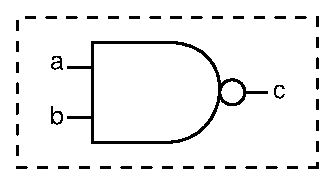
\includegraphics[scale=0.5]{nand2}
&
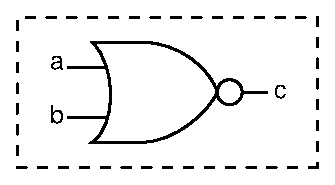
\includegraphics[scale=0.5]{nor2}
\\
\begin{minipage}[b]{2.5in}
\begin{ocamllisting}
class nand2 =
object
   inherit two_input_gate
   method compute_value = not (a && b)
end
\end{ocamllisting}
\end{minipage}
&
\begin{minipage}[b]{2.5in}
\begin{ocamllisting}
class nor2 =
object
   inherit two_input_gate
   method compute_value = not (a || b)
end
\end{ocamllisting}
\end{minipage}
\end{tabular}
\end{center}
%
\begin{enumerate}
\item 
Fill in the definitions of the methods \hbox{\lstinline/connect_input_a/} and \hbox{\lstinline/connect_input_b/}.

\begin{answer}\ifanswers
For the methods \hbox{\lstinline/connect_input_a/} we need to construct a terminal object
that performs the appropriate action.
\begin{ocaml}
   method connect_input_a (wire : wire) =
       wire#add_terminal (object method set x = self#set_input_a x end)
\end{ocaml}
\fi\end{answer}

\item
Define a class \hbox{\lstinline/three_input_gate/} (for gates with three inputs) by inheriting
from \hbox{\lstinline/two_input_gate/}.
\begin{answer}\ifanswers
\begin{ocaml}
class three_input_gate =
object
   inherit two_input_gate
   val mutable c = false
   method private set_input_c x = c <- x; self#set_output
   method connect_input_c (wire : wire) =
       wire#add_terminal (object method set x = self#set_input_c x end)
\end{ocaml}
\fi\end{answer}
   
\item
Would the definition be simpler if the type \hbox{\lstinline/terminal/} were a function instead of an
object (where \hbox{\lstinline/type terminal = bool -> unit/})?

\begin{answer}\ifanswers
It would be slightly simpler because the input terminal could be set without the intermediate terminal object.
The connect methods would have the following form.

\begin{ocaml}
   method connect_input_a (wire : wire) =
      wire#add_terminal self#set_input_a
\end{ocaml}
\fi\end{answer}

\item
What is the purpose of the conditional \hbox{\lstinline/if x <> value then $\cdots$/} in the class \hbox{\lstinline/wire/}?

\begin{answer}\ifanswers
The conditional prevents activity from propagating if it does not change the circuit values.
It also means that the simulation will terminate, even for cyclic circuits, if the circuit becomes quiescent.
\fi\end{answer}

\item
Write a program for the following circuit, called a \emph{SR latch}.
\begin{center}
\begin{tabular}{cc}
\begin{tabular}[b]{cc|c}
S & R & Action\\
\hline
0 & 0 & Keep state\\
0 & 1 & $Q = 0$\\
1 & 0 & $Q = 1$\\
1 & 1 & $Q = 0, \overline{Q} = 0$\\
\\
\end{tabular}
&
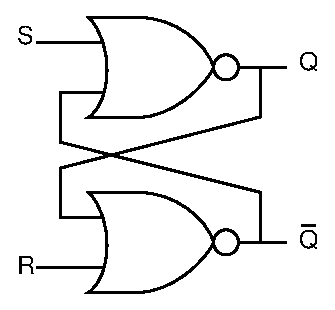
\includegraphics[scale=0.5]{latch}
\end{tabular}
\end{center}

\begin{answer}\ifanswers
\begin{ocaml}
let gate1 = new nor2;;
let gate2 = new nor2;;
let wire1 = new wire;;
let wire2 = new wire;;
gate1#connect_output wire1;;
gate2#connect_output wire2;;
gate1#connect_input_b wire2;;
gate2#connect_input_a wire1;;
\end{ocaml}
\fi\end{answer}
\end{enumerate}
\end{exercise}
   
\begin{exercise}{event-driven-simulator}
The simulator in Exercise~\ref{exercise:circuit-simulation}
has a problem with some cyclic circuits.  For example, the following circuit,
called a \emph{ring oscillator}, oscillates indefinitely, overflowing the stack during simulation.

\begin{center}
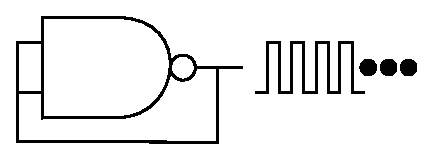
\includegraphics[scale=0.5]{ring}
\end{center}
%
The simulation can be executed in constant stack space by implementing an \emph{event-driven
simulator}.  In the circuit context, an \emph{event} occurs whenever the value on a terminal is set.
An event-driven simulator uses a scheduler to manage events.  When the value of a terminal is set,
the terminal is scheduled, but not executed yet.  When scheduled, the terminal is removed from the
scheduling queue and executed.

Define an event driven simulator by implementing a scheduler.  You can use a scheduling policy of
your choice, but it should be fair, meaning that if a terminal is scheduled, it will eventually be
executed.  

The scheduler should include a method \hbox{\lstinline/main : unit/} that runs until there are no more
events (perhaps forever).  The type \hbox{\lstinline/terminal/} should be defined as follows.
The method \hbox{\lstinline/set/} schedules the terminal, and the method \hbox{\lstinline/execute/} executes it.

\begin{ocaml}
type terminal = < set : bool -> unit; execute : unit >
\end{ocaml}

\begin{answer}\ifanswers
The scheduling queue can be implemented using the \hbox{\lstinline/Queue/} standard library.
This will use a FIFO policy, which is fair.

The scheduler has two methods.  The method \hbox{\lstinline/main/} runs the simulation until the
queue is empty.  The method \hbox{\lstinline/connect_input/} takes a wire and a function, creates
a terminal object, and add the object to the wire.  When the terminal is set, it gets
added to the scheduling queue.  Note that the field \hbox{\lstinline/event_queue/} is accessible
in the inner terminal object.

\begin{ocaml}
type terminal = < set : bool -> unit; execute : unit >

class scheduler =
object (self : 'self)
   val event_queue : terminal Queue.t = Queue.create ()

   method main =
       while not (Queue.is_empty event_queue) do
          (Queue.take event_queue)#execute
       done
   method connect_input (wire : wire) (f : bool -> unit) =
      let term =
         object (term_self)
            val mutable value = false
            method set x =
               value <- x;
               Queue.add term_self event_queue
            method execute = f value
         end
      in
      wire#add_terminal term
end;;

let the_scheduler = new scheduler;;
\end{ocaml}
%
The only other change to the simulation is to the methods \hbox{\lstinline/connect_input_?/}.

\begin{ocaml}
class virtual two_input_gate =
object (self : 'self)
   inherit gate
   val mutable a = false
   val mutable b = false
   method private set_input_a x = a <- x; self#set_output
   method private set_input_b x = b <- x; self#set_output
   method connect_input_a (wire : wire) =
      the_scheduler#connect_input wire self#set_input_a
   method connect_input_b (wire : wire) =
      the_scheduler#connect_input wire self#set_input_b
end
\end{ocaml}
\fi\end{answer}
\end{exercise}

% -*-
% Local Variables:
% Mode: LaTeX
% fill-column: 100
% TeX-master: "paper"
% TeX-command-default: "LaTeX/dvips Interactive"
% End:
% -*-
% vim:tw=100:fo=tcq:

\exercises

%%%%%%%%%%%%%%%%%%%%%%%%%%%%%%%%%%%%%%%%%%%%%%%%%%%%%%%%%%%%%%%%%%%%%%%%
% Names
%
\begin{exercise}{person-name}
Assume there is a class \hbox{\lstinline/name/} that represents the
name of a person.  We would normally say that a \hbox{\lstinline/person/} is-a \hbox{\lstinline/human/} and has-a \hbox{\lstinline/name/},

\begin{ocaml}
class person (n : name) = object inherit human val name = n $\cdots$ end
\end{ocaml}
%
Suppose that instead, the class \hbox{\lstinline/person/} inherits from both.

\begin{ocaml}
class person (s : string) =
object
   inherit human
   inherit name s
   $\cdots$
end
\end{ocaml}
%
What is the difference?  Under what conditions would the different
representations be preferred?

\begin{answer}\ifanswers
In the former case, a person is not a name, and can't be used as a
name.  With multiple inheritance, the person \emph{can} be used as a
name.  Multiple inheritance is more likely to be used in a situation
where the name of a person and the person himself are treated as the
same thing.  The former is more likely when the name is just a symbol
for the person.
\fi\end{answer}
\end{exercise}

%%%%%%%%%%%%%%%%%%%%%%%%%%%%%%%%%%%%%%%%%%%%%%%%%%%%%%%%%%%%%%%%%%%%%%%%
% Reference counting
%
\begin{exercise}{reference-counting}
Consider the following class, which implements a persistent
reference-counted value stored in a file.  When there are no more
references, the file is removed.

\begin{ocaml}
class persistent_refcounted_value filename =
object (self)
    (* persistent_value *)
    val mutable x : int list =
       let fin = open_in_bin filename in
       let x = input_value fin in
       close_in fin;
       x
    method get = x
    method set y = x <- y; self#save
    method private save =
       let fout = open_out_bin filename in
       output_value fout x;
       close_out fout

    (* refcounted_value *)
    val mutable ref_count = 1
    method add_ref = ref_count <- ref_count + 1
    method rm_ref =
       ref_count <- ref_count - 1;
       if ref_count = 0 then
          Sys.remove filename
end
\end{ocaml}
%
\begin{enumerate}
\item Partition the class into three classes: \hbox{\lstinline/persistent_value/} implements
persistent values stored in files, \hbox{\lstinline/refcounted_value/} implements generic reference
counted objects, and \hbox{\lstinline/persistent_refcounted_value/} inherits from both.

\item What is the advantage in partitioning the class?
\end{enumerate}

\begin{answer}\ifanswers
\begin{enumerate}
\item
The class is simply split down the middle.  The details of deletion must be implemented by
the value, not the reference counting class, so the virtual method \hbox{\lstinline/delete/} is
used to connect the two objects.

\begin{ocaml}
class persistent_value filename =
object (self)
    val mutable x : int list =
       let fin = open_in_bin filename in
       let x = input_value fin in
       close_in fin;
       x
    method get = x
    method set y = x <- y; self#save
    method private save =
       let fout = open_out_bin filename in
       output_value fout x;
       close_out fout
    method private delete = Sys.remove filename
end

class virtual ref_value =
object (self)
    val mutable ref_count = 1
    method add_ref = ref_count <- ref_count + 1
    method rm_ref =
       ref_count <- ref_count - 1;
       if ref_count = 0 then self#delete
    method private virtual delete : unit
end

class persistent_ref_value2 filename =
object
   inherit persistent_value filename
   inherit ref_value
end
\end{ocaml}

\item The advantage of splitting the class is that we now have two more generic classes.
For example, reference counting is general concept that can be re-used elsewhere in the program.
\end{enumerate}
\fi\end{answer}
\end{exercise}

%%%%%%%%%%%%%%%%%%%%%%%%%%%%%%%%%%%%%%%%%%%%%%%%%%%%%%%%%%%%%%%%%%%%%%%%
% Programmer
%
\begin{exercise}{french-programmer}
In the French programmer example, the \hbox{\lstinline/programmer/} has a
field \hbox{\lstinline/favorite_language/} and so does
the \hbox{\lstinline/french_person/}.  Can the inheritance hierarchy be
modified so that these are available
as \hbox{\lstinline/favorite_programming_language/}
and \hbox{\lstinline/favorite_natural_language/}, without
modifying the classes \hbox{\lstinline/programmer/} and \hbox{\lstinline/french_person/}?

\begin{answer}\ifanswers
OCaml doesn't provide a way to rename fields, so the only thing we can
do is to hide the field and use methods to access it.  Suppose the
class \hbox{\lstinline/programmer/} is defined as follows.

\begin{ocaml}
class programmer =
object
   inherit person
   val favorite_language = "OCaml"
end
\end{ocaml}
%
The renamed class \hbox{\lstinline/programmer'/} could be defined as follows.

\begin{ocaml}
class type programmer_type' =
object
   val name : string
   val address : string
   method favorite_programming_language : string
end

class programmer' : programmer_type' =
object
   inherit programmer
   method favorite_programming_language = favorite_language
end
\end{ocaml}
\fi\end{answer}
\end{exercise}

%%%%%%%%%%%%%%%%%%%%%%%%%%%%%%%%%%%%%%%%%%%%%%%%%%%%%%%%%%%%%%%%%%%%%%%%
% Lists
%
\begin{exercise}{multiple-list}
You are given the following functor that defines a class \hbox{\lstinline/cell/}
containing a value of type \hbox{\lstinline/T.t/}.

\begin{ocaml}
module MakeCell (T : sig type t end) =
struct
    class cell x =
    object
        val mutable x : T.t = x
        method private get = x
        method private set y = x <- y
    end
end
\end{ocaml}
%
Define a singly-linked list of integers by inheriting from the class \hbox{\lstinline/cell/}
twice.  Your class should have the type \hbox{\lstinline/int_cons/}.

\begin{ocaml}
class type int_cons =
object
   method hd : int
   method tl : int_cons option
   method set_hd : int -> unit
   method set_tl : int_cons option -> unit
end

type int_list = int_cons option
\end{ocaml}

\begin{answer}\ifanswers
Inheriting from the \hbox{\lstinline/cell/} twice would override the
methods \hbox{\lstinline/get/} and \hbox{\lstinline/set/}, which is not what we
want.  We need to \emph{rename} the methods first.  For this list, it
is sufficient to rename the methods in just one of the classes.  Note
that the cell value is hidden so that it is not overridden.

\begin{ocaml}
module IntCell =
struct
   module Cell = MakeCell (struct type t = int end);;

   class type cell_type =
   object
      method private get_int : int
      method private set_int : int -> unit
   end

   class cell i : cell_type =
   object (self)
      inherit Cell.cell i
      method private get_int = self#get
      method private set_int = self#set
   end
end

module ListCell = MakeCell (struct type t = int_list end);;

class cons i : int_cons =
object
    inherit IntCell.cell i as value
    inherit ListCell.cell None as link

    method hd = value#get_int
    method tl = link#get
    method set_hd = value#set_int
    method set_tl = link#set
end
\end{ocaml}
\fi\end{answer}
\end{exercise}    
    
%%%%%%%%%%%%%%%%%%%%%%%%%%%%%%%%%%%%%%%%%%%%%%%%%%%%%%%%%%%%%%%%%%%%%%%%
% Recursive functions
%
\begin{exercise}{multiple-recursive-functions}
Suppose we have several mutually-recursive functions 
\hbox{\lstinline/$f_1$ : int -> int/}, $\ldots$, \hbox{\lstinline/$f_n$ : int -> int/}
that we want to define in separate files.  In
Exercise~\ref{exercise:functor5} we did this with recursive modules.
Do it with multiple inheritance instead.  Is there any advantage to
using classes over recursive modules?

\begin{answer}\ifanswers
Each function $f_i : int -> int$ would be defined in a separate class,
where all the other functions are virtual.

\begin{ocaml}
class virtual fun_$i$ =
object
   method virtual $f_1$ : int -> int
   $\cdots$
   method virtual $f_{i - 1}$ : int -> int
   method $f_i$ i = $\cdots$
   $\cdots$
   method virtual $f_n$ : int -> int
end
\end{ocaml}
%
The final class would use multiple inheritance to tie the recursive knot.
%
\begin{ocaml}
class everything =
object
   inherit fun_$1$ $\cdots$ inherit fun_$n$
end
\end{ocaml}
%
To reduce the amount of code, a single shared base class could be used
to declare all the functions.

\begin{ocaml}
class virtual declarations =
object
   method virtual $f_1$ : int -> int
   $\cdots$
   method virtual $f_n$ : int -> int
end

class virtual fun_$i$ =
object
   inherit declarations
   method $f_i$ i = $\cdots$
end
\end{ocaml}
%
An advantage of the class representation is that the text required
for the declarations is \emph{much} smaller than needed for recursive
modules.
\fi\end{answer}
\end{exercise}

% -*-
% Local Variables:
% Mode: LaTeX
% fill-column: 100
% TeX-master: "paper"
% TeX-command-default: "LaTeX/dvips Interactive"
% End:
% -*-
% vim:tw=100:fo=tcq:

%
%
%
%%%%%%%%%%%%%%%%%%%%%%%%%%%%%%%%%%%%%%%%%%%%%%%%%%%%%%%%%%%%%%%%%%%%%%%%
% Exercises
%

\exercises

\begin{exercise}{poly-fields}
The restriction about free type variables applies only to non-private method
types.  Which of the following definitions are legal?  For those that
are legal, give their types.  For those that are not legal, explain
why.

\begin{enumerate}
\item

\begin{ocamllisting}
class c1 = object val x = [] end;;
\end{ocamllisting}

\item

\begin{ocamllisting}
class c2 = object val x = ref [] end;;
\end{ocamllisting}

\item

\begin{ocamllisting}
class c3 x = object val y = x end
\end{ocamllisting}

\item

\begin{ocamllisting}
class c4 x = object val y = x method z = y end
\end{ocamllisting}

\item

\begin{ocamllisting}
class c5 x = object val y = x + 1 method z = y end
\end{ocamllisting}

\item

\begin{ocamllisting}
class c6 (x : 'a) = object constraint 'a = int method y = x end;;
\end{ocamllisting}
\end{enumerate}

\begin{answer}\ifanswers
\begin{enumerate}
\item

Legal; the type is \hbox{\lstinline$class c1 : object val x : 'a list end$}

\item

Legal; the type produced by the toploop is

\begin{ocaml}
class c2 : object val x : 'a list ref end
\end{ocaml}
%
This typing seems a little strange, since \hbox{\lstinline$x$} is not truly
polymorphic (its type should be \hbox{\lstinline$'_a list ref$}).

\item

Legal; the type is \hbox{\lstinline$class c3 : 'a -> object val y : 'a end$}.

\item

Not legal; the method \hbox{\lstinline$z$} has a polymorphic
type \hbox{\lstinline$'a$}, which is not a parameter of the class definition.

\item

Legal; the type is
\hbox{\lstinline$class c5 : int -> object val y : int method z : int end$}.

\item

Legal; the constraint means the class type is not polymorphic.  The type
is \hbox{\lstinline$class c6 : int -> object method y : int end$}.
\end{enumerate}
\fi\end{answer}
\end{exercise}

%%%%%%%%%%%%%%%%%%%%%%%%%%%%%%%%%%%%%%%%%%%%%%%%%%%%%%%%%%%%%%%%%%%%%%%%

\begin{exercise}{poly-imperative-map}
Write an imperative version of a polymorphic map.  A newly-created map
should be empty.  The class should have the following type.

\begin{ocaml}
class ['a, 'b] imp_map : ('a -> 'a -> ordering) ->
  object
    method find   : 'a -> 'b
    method insert : 'a -> 'b -> unit
  end
\end{ocaml}

\begin{answer}\ifanswers
Here is one implementation.

\begin{ocaml}
class ['key, 'value] imp_map (compare : 'key -> 'key -> comparison) =
   let equal key1 (key2, _) = compare key1 key2 = Equal in
   object (self : 'self)
      val mutable elements : ('key * 'value) list = []
      method insert key value = elements <- (key, value) :: elements
      method find key = snd (List.find (equal key) elements)
   end;;
\end{ocaml}
\fi\end{answer}
\end{exercise}

%%%%%%%%%%%%%%%%%%%%%%%%%%%%%%%%%%%%%%%%%%%%%%%%%%%%%%%%%%%%%%%%%%%%%%%%

\begin{exercise}{virtual-compare1}
Reimplement the polymorphic map class from page~\pageref{page:poly-map}
so that the class takes no arguments, and \hbox{\lstinline$compare$} is a
virtual method.  Define a specific class \hbox{\lstinline$int_map$} where
the keys have type \hbox{\lstinline$int$} with the usual ordering.

\begin{answer}\ifanswers
When \hbox{\lstinline$compare$} is implemented as a method, the equality
function \hbox{\lstinline$equal$} must also be a method.  

\begin{ocaml}
class virtual ['key, 'value] map =
  object (self : 'self)
    val elements : ('key * 'value)
    method add key value = {< elements = (key, value) :: elements >}
    method find key = snd (List.find (self#equal key) elements)

    method private equal key1 (key2, _) = compare key1 key2 = Equal
    method private virtual compare : 'key -> 'key -> ordering
  end;;

class ['value] int_map =
  object (self : 'self)
    inherit [int, 'value] map

    method private compare i j =
      if i < j then Smaller
      else if i > j then Larger
      else Equal
  end
\end{ocaml}
\fi\end{answer}
\end{exercise}

%%%%%%%%%%%%%%%%%%%%%%%%%%%%%%%%%%%%%%%%%%%%%%%%%%%%%%%%%%%%%%%%%%%%%%%%

\begin{exercise}{polyclasses-self1}
In the class type definition \hbox{\lstinline$['a] tree$} on
page~\pageref{page:poly-tree}, the method \hbox{\lstinline$add$} has
type \hbox{\lstinline$'a -> 'a tree$}.  What would happen if we defined the
class type as follows?

\begin{ocaml}
class type ['a] self_tree =
  object ('self)
    method add : 'a -> 'self
    method mem : 'a -> bool
  end
\end{ocaml}

\begin{answer}\ifanswers
The alternate definition, using \hbox{\lstinline$'self$} does not work because
the class \hbox{\lstinline$leaf$} must create a new internal node.  The expression
\hbox{\lstinline$new node x (self :> 'a tree) (self : 'a tree)$} has type
\hbox{\lstinline$'a tree$}.  It doesn't have type \hbox{\lstinline$'self$}.
\fi\end{answer}
\end{exercise}

%%%%%%%%%%%%%%%%%%%%%%%%%%%%%%%%%%%%%%%%%%%%%%%%%%%%%%%%%%%%%%%%%%%%%%%%

\begin{exercise}{object-tree-compare}
In the implementations for the \hbox{\lstinline$['a] node$}
and \hbox{\lstinline$['a] leaf$} classes in
Section~\reflabelsection{polymorphic-class-types}, the
function \hbox{\lstinline$compare$} is threaded through the class
definitions.  Implement a functor \hbox{\lstinline$MakeTree$},
specified as follows.

\begin{ocaml}
type ordering = Smaller | Equal | Larger

module type CompareSig = sig
   type t
   val compare : t -> t -> ordering
end;;

class type ['a] tree =
  object ('self)
    method add : 'a -> 'a tree
    method mem : 'a -> bool
  end;;

module MakeTree (Compare : CompareSig)
  : sig val empty : Compare.t tree end =
struct $\cdots$ end
\end{ocaml}

\begin{answer}\ifanswers
\begin{ocaml}
module MakeTree (Compare : CompareSig)
  : sig val empty : Compare.t tree end =
struct
   open Compare
   type key = Compare.t
   type t = key tree

   class node x (l : t) (r : t) =
     object (self : 'self)
       val label = x
       val left = l
       val right = r
       method mem x =
         match compare x label with
            Smaller -> left#mem x
          | Larger -> right#mem x
          | Equal -> true
       method add x =
         match compare x label with
            Smaller -> {< left = left#add x >}
          | Larger -> {< right = right#add x >}
          | Equal -> self
   end;;

   class leaf =
     object (self : 'self)
       method mem _ = false
       method add x = new node x (self :> t) (self :> t)
     end;;

   let empty = new leaf;;
end;;
\end{ocaml}
\fi\end{answer}
\end{exercise}

%%%%%%%%%%%%%%%%%%%%%%%%%%%%%%%%%%%%%%%%%%%%%%%%%%%%%%%%%%%%%%%%%%%%%%%%

\begin{exercise}{object-tree-virtual}
Instead of defining a class type \hbox{\lstinline$class type ['a] tree$},
we could have specified it as a virtual class like the following.

\begin{ocaml}
class virtual ['a] virtual_tree =
  object (self : 'self)
    method virtual add : 'a -> 'a virtual_tree
    method virtual mem : 'a -> bool
  end;;
\end{ocaml}
%
Are there any advantages or disadvantages to this approach?

\begin{answer}\ifanswers
The new definition is nearly the same.  However, class definitions,
even virtual ones, are not allowed in signatures or interfaces
(\hbox{\lstinline$.mli$} files), so there is a disadvantage to using the
virtual class specification.
\fi\end{answer}
\end{exercise}

%%%%%%%%%%%%%%%%%%%%%%%%%%%%%%%%%%%%%%%%%%%%%%%%%%%%%%%%%%%%%%%%%%%%%%%%

\begin{exercise}{variance-annotations1}
Which of the following class definitions are legal?  Explain your answers.

\begin{enumerate}
\item

\begin{ocamllisting}
class [+'a] cl (x : 'a) =
  object (self : 'self)
    val f : 'a -> unit = fun x -> ()
    method value : unit -> 'a = fun () -> x
  end
\end{ocamllisting}

\item 

\begin{ocamllisting}
class [+'a] cl =
  object (self : 'self)
    method f : 'a -> unit = fun x -> ()
  end
\end{ocamllisting}

\item

\begin{ocamllisting}
class [+'a] cl =
  object (self : 'self)
    method private f : 'a -> unit = fun x -> ()
  end
\end{ocamllisting}

\item

\begin{ocamllisting}
class [+'a] cl =
  object (self : 'a)
    method copy : 'a = {< >}
  end
\end{ocamllisting}

\item

\begin{ocamllisting}
class [-'a] cl (x : 'a) =
  object (self : 'self)
    val mutable y = x
    method f x = y <- x
  end;;
\end{ocamllisting}

\item

\begin{ocamllisting}
class foo = object end
class ['a] cl (x : 'a) =
  object
    constraint 'a = #foo
    method value : #foo = x
  end
\end{ocamllisting}

\item

\begin{ocamllisting}
class foo = object end
class [-'a] cl (x : #foo as 'a) =
  object
    method value : #foo = x
  end
\end{ocamllisting}

\end{enumerate}

\begin{answer}\ifanswers
\begin{enumerate}
\item The annotation is legal, because fields are not part of the variance calculation.
\item The annotation is not legal, the type variable \hbox{\lstinline$'a$} occurs negatively.
\item The annotation is legal, because private methods are not part of the variance calculation.
\item The annotation is legal.
\item The annotation is legal, because \hbox{\lstinline$'a$} occurs only negatively in the type of the method \hbox{\lstinline$f$}.
\item The annotation is legal.
\item The annotation is not legal, because the type \hbox{\lstinline$#foo$} must be covariant.
\end{enumerate}
\fi\end{answer}
\end{exercise}

%%%%%%%%%%%%%%%%%%%%%%%%%%%%%%%%%%%%%%%%%%%%%%%%%%%%%%%%%%%%%%%%%%%%%%%%

\begin{exercise}{animal-pair1}
Consider the following class definitions.

\begin{center}
\begin{tabular}{cc}
\begin{minipage}[t]{2.8in}
\begin{ocamllisting}
class ['a] alt_animal_pair1 (p : 'a) =
  object (self : 'self)
    constraint 'a = ('b, 'b) #pair
    constraint 'b = #animal
    method sleep =
      let a1, a2 = p#value in
      a1#sleep; a2#sleep
  end;;
\end{ocamllisting}
\end{minipage}
&
\begin{minipage}[t]{2.2in}
\begin{ocamllisting}
class ['a] alt_animal_pair2
  (a1 : 'b) (a2 : 'c) =
  object (self : 'self)
    inherit ['b, 'c] pair a1 a2
    constraint 'a = 'b * 'c
    constraint 'b = #animal
    constraint 'c = #animal
    method sleep =
      a1#sleep; a2#sleep
  end;;
\end{ocamllisting}
\end{minipage}
\end{tabular}
\end{center}
%
\begin{enumerate}
\item

The type variable \hbox{\lstinline$'b$} is not a type parameter
of \hbox{\lstinline$alt_animal_pair1$}.  Why is the definition legal?

\item

Is the type \hbox{\lstinline$['a] alt_animal_pair1$} covariant, contravariant, or invariant in \hbox{\lstinline$'a$}?

\item

Suppose we have a class \hbox{\lstinline$cat$} that is a subtype of \hbox{\lstinline$animal$}.
What is the type of the following expression?

\begin{ocaml}
new alt_animal_pair2 (new dog "Spot") (new cat "Fifi");;
\end{ocaml}

\item

What happens if the line \hbox{\lstinline$constraint 'a = 'b * 'c$} is left out
of the class definition for \hbox{\lstinline$alt_animal_pair2$}?

\item

What if the line is replaced with \hbox{\lstinline$constraint 'a = 'b -> 'c$}?

\item

In principle, is it ever necessary for a class to have more than one
type parameter?
\end{enumerate}

\begin{answer}\ifanswers
\begin{enumerate}
\item 

The definition is legal because the type variable \hbox{\lstinline$'b$} is
included as a part of \hbox{\lstinline$'a$}, so \hbox{\lstinline$'b$} is not free in
the definition.

\item

Technically, all three annotations \hbox{\lstinline$+'a$}, \hbox{\lstinline$-'a$},
and \hbox{\lstinline$'a$} are accepted.  However, since the
type \hbox{\lstinline$('b, 'b) pair$} is covariant in \hbox{\lstinline$'b$}, the
definition is also covariant in \hbox{\lstinline$'a$}.

\item

The type is \hbox{\lstinline$(dog * cat) alt_animal_pair2$}.  Note that the
type \hbox{\lstinline$dog * cat$} is artificial, it has nothing to do
with whether the class represents a pair.

\item

If the constraint is left out, the type variables \hbox{\lstinline$'b$}
and \hbox{\lstinline$'c$} become free in the class definition, so the
definition is rejected.

\item

The constraint \hbox{\lstinline$constraint 'a = 'b -> 'c$} is also legal, but
it means that the definition is no longer covariant in \hbox{\lstinline$'a$}.

\item

Strictly speaking, it isn't necessary.  Suppose we have a class type
\hbox{\lstinline/[-'a1, $\ldots$, -'an, +'b1, $\ldots$, +'bm] cl/}.
We can replace it with a single constraint \hbox{\lstinline/['c] cl/}
and the following constraint.

\begin{ocaml}
constraint 'c = ('a1 * $\cdots$ * 'an) -> ('b1 * $\cdots$ * 'bn)
\end{ocaml}
%
We can't specify the variance of \hbox{\lstinline$'c$}, but the constraint
enforces the variance.
\end{enumerate}
\fi\end{answer}
\end{exercise}

%%%%%%%%%%%%%%%%%%%%%%%%%%%%%%%%%%%%%%%%%%%%%%%%%%%%%%%%%%%%%%%%%%%%%%%%

\begin{exercise}{env-variance}
In the object implementation of the evaluator in
Figure~\reffigure{implementing-evaluator}, the method \hbox{\lstinline$eval$}
takes an environment of exact type \hbox{\lstinline$int env$}.  Suppose we
try to change it to the following definition.

\begin{ocaml}
class type exp =
  object ('self)
    method eval : int #env -> int
  end

class int_exp (i : int) : exp =
  object (self : 'self)
    method eval (_ : int #env) = i
  end;;
$\cdots$
\end{ocaml}
%
\begin{enumerate}
\item

The new type definition is accepted, but the class
definition \hbox{\lstinline$int_exp$} is rejected.  How can it be fixed?

\item Are there any advantages to the new definition?
\end{enumerate}

\begin{answer}\ifanswers
\begin{enumerate}
\item

The problem is that the type \hbox{\lstinline$#env$} is polymorphic.
We can fix the definition by using a polymorphic method type.

\begin{ocaml}
class int_exp (i : int) : exp =
  object (self : 'self)
    method eval : 'a. (int #env as 'a) -> int = (fun _ -> i)
  end;;
\end{ocaml}

\item

There isn't really any reason to use the new definition, because 
an environment of type \hbox{\lstinline$int #env$} is no more useful than
an environment of type \hbox{\lstinline$int env$}.  The only savings is
in the outermost call to the evaluator, where is may be possible
to omit a coercion.
\end{enumerate}
\fi\end{answer}
\end{exercise}

%%%%%%%%%%%%%%%%%%%%%%%%%%%%%%%%%%%%%%%%%%%%%%%%%%%%%%%%%%%%%%%%%%%%%%%%

\begin{exercise}{monoclasses}
Consider the following class definition.

\begin{ocaml}
# class type ['a] c1 = object method f : c2 -> 'a end
  and c2 = object method g : int c1 end;;
@
\begin{topoutput}
class type ['a] c1 = object constraint 'a = int method f : c2 -> 'a end
and c2 = object method g : int c1 end
\end{topoutput}
@
\end{ocaml}
%
Unfortunately, even though the class type \lstinline$['a] c1$ should
be polymorphic in \hbox{\lstinline$'a$}, a type constraint is inferred
that \hbox{\lstinline$'a = int$}.  The problem is that polymorphic
type definitions are not polymorphic \emph{within} a recursive
definition.

\begin{enumerate}
\item

Suggest a solution to the problem, where class type \lstinline$c1$ is
truly polymorphic.

\item

The following definition is rejected.

\begin{ocaml}
# class type ['a] c1 = object method f : c2 -> 'a end
  and c2 = object method g : 'a. 'a c1 -> 'a end;;
@
\begin{toperror}
Characters 79-94:
and c2 = object method g : 'a. 'a c1 -> 'a end;;
                           ^^^^^^^^^^^^^^^
This type scheme cannot quantify 'a :
it escapes this scope.
\end{toperror}
@
\end{ocaml}
%
The problem arises from the same issue---the class \lstinline$['a] c1$
is not polymorphic within the recursive definition, so the
type \lstinline$'a. 'a c1 -> 'a$ is rejected.

Suggest a solution to this problem.
\end{enumerate}

\begin{answer}\ifanswers
The solution in both cases is to break apart the recursive definition
by adding a type parameter to the class type \lstinline$c1$ that represents
the class \hbox{\lstinline$c2$}.

\begin{ocaml}
class type ['a, 'c2] pre_c1 = object method f : 'c2 -> 'a end
\end{ocaml}
%
The solutions are then as follows.

\begin{enumerate}
\item

\begin{ocamllisting}
class type c2 = object method g : (int, c2) pre_c1 end
class type ['a] c1 = ['a, c2] pre_c1
\end{ocamllisting}

\item

\begin{ocamllisting}
class type c2 = object method g : 'a. ('a, c2) pre_c1 -> 'a end
class type ['a] c1 = ['a, c2] pre_c1
\end{ocamllisting}
\end{enumerate}
\fi\end{answer}
\end{exercise}

%%%%%%%%%%%%%%%%%%%%%%%%%%%%%%%%%%%%%%%%%%%%%%%%%%%%%%%%%%%%%%%%%%%%%%%%

\begin{exercise}{visitor-pattern}
As discussed in
Section~\reflabelsection{comparing-objects-and-modules}, one problem
with object-oriented implementations is that adding a new functionality
to a class hierarchy might require modifying all the classes
in the hierarchy.  \emph{Visitor design patterns} are one way in
which this problem can be addressed.

A \emph{visitor} is defined as an object with a method for each of the
kinds of data.  For the type \hbox{\lstinline$exp$}, a visitor would have the
following type.

\begin{ocaml}
class type visitor =
  object ('self)
    method visit_int : int_exp -> unit
    method visit_var : var_exp -> unit
    method visit_add : add_exp -> unit
    method visit_if  : if_exp  -> unit
    method visit_let : let_exp -> unit
  end;;
\end{ocaml}
%
The class type \hbox{\lstinline$exp$} is augmented with a
method \hbox{\lstinline$accept : visitor -> unit$} that guides the
visitor through an expression, visiting every subexpression in turn.
Here is a fragment of the code.

\begin{ocaml}
class type exp =
  object ('self)
    method eval : int env -> int
    method accept : visitor -> unit
  end;;

class int_exp (i : int) =
  object (self : 'self)
    method eval (_ : int env) = i
    method accept visitor = visitor#visit_int (self :> int_exp)
  end

class add_exp (e1 : #exp) (e2 : #exp) =
  object (self : 'self)
    method eval env = e1#eval env + e2#eval env
    method accept visitor =
      visitor#visit (self :> add_exp);
      e1#accept visitor;
      e2#accept visitor
  end
$\cdots$
\end{ocaml}

\begin{enumerate}
\item[1.]

One problem with this approach is the order of definitions.  For
example, the class type \hbox{\lstinline$visitor$} refers to the
class \hbox{\lstinline$add_exp$}, which refers back to
the \hbox{\lstinline$visitor$} type in the definition of the
method \hbox{\lstinline$accept$}.

\begin{enumerate}
\item We could simplify the types.  Would the following definition be acceptable?

\begin{ocaml}
class type exp =
  object ('self)
    method eval : int env -> int
    method accept : visitor -> unit
  end

and visitor =
  object ('self)
    method visit_int : exp -> unit
    method visit_var : exp -> unit
    $\cdots$
  end
\end{ocaml}

\item

What is a better way to solve this problem?
\end{enumerate}

\item[2.]

The class type \hbox{\lstinline$visitor$} has one method for each specific
kind of expression.  What must be done when a new kind of expression
is added?
\end{enumerate}
%
As defined, the visitor pattern is not very useful because the classes
do not provide any additional information about themselves.  Suppose
we add a method \hbox{\lstinline$explode$} that presents the contents
of the object as a tuple.  Here is a fragment.

\begin{ocaml}
class type exp = object $\cdots$ end
and visitor = object $\cdots$ end

and int_exp_type =
  object ('self)
    inherit exp
    method explode : int
  end

and add_exp_type =
  object ('self)
    inherit exp
    method explode : exp * exp
  end
$\cdots$
\end{ocaml}

\begin{enumerate}
\item[3.]

Since the method \hbox{\lstinline$explode$} exposes the internal representation,
it isn't really necessary for the \hbox{\lstinline$accept$} methods to perform the
recursive calls.  For example, we could make the following definition,
and assume that the visitor will handle the recursive calls itself.

\begin{ocaml}
class add_exp (e1 : #env) (e2 : #env) : add_exp_type =
  object (self : 'self)
    method eval env = e1#eval env + e2#eval env
    method accept visitor = visitor#visit_add (self :> add_exp_type)
    method explode = e1, e2
  end
\end{ocaml}
%
What are the advantages of this approach?  What are its disadvantages?

\item[4.]

Another approach is, instead of passing the objects directly to the
visitor, to pass the exploded values as arguments.  Here is the new visitor
type definition.

\begin{ocaml}
class type visitor =
  object ('self)
    method visit_int : int -> unit
    method visit_add : exp -> exp -> unit
    $\cdots$
  end
\end{ocaml}
%
What are the advantages of this approach?  What are its disadvantages?

\item[5.]

Write a visitor to print out an expression.
\end{enumerate}
%
The visitors we have specified are imperative.  It is also possible to
write pure visitors that compute without side-effects.  The visitor
has a polymorphic class type parameterized over the type of values it
computes.  As discussed in Exercise~\ref{exercise:monoclasses}, a recursive
definition does not work, so we break apart the recursive definition.

\begin{ocaml}
class type ['a, 'exp] pre_visitor =
  object ('self)
    method visit_int : int -> 'a
    method visit_var : string -> 'a
    method visit_add : 'exp -> 'exp -> 'a
    method visit_if  : 'exp -> 'exp -> 'exp -> 'a
    method visit_let : string -> 'exp -> 'exp -> 'a
  end;;

class type exp =
  object ('self)
    method eval   : int env -> int
    method accept : 'a. ('a, exp) pre_visitor -> 'a
  end

class type ['a] visitor = ['a, exp] pre_visitor
\end{ocaml}

\begin{enumerate}
\item[6.]

Rewrite the class definitions to implement the new \hbox{\lstinline$accept$} methods.

\item[7.]

Write an evaluator as a pure visitor \hbox{\lstinline$eval_visitor$}.
The \hbox{\lstinline$eval_visitor$} is not allowed to call the
method \hbox{\lstinline$eval$}, and it is not allowed to use assignment or
any other form of side-effect.
\end{enumerate}

\begin{answer}\ifanswers
\begin{enumerate}
\item

\begin{enumerate}
\item
The simplified class type \hbox{\lstinline$visitor$} is not acceptable because the
visitor methods are called with a plain expression \hbox{\lstinline$exp$}, which
isn't enough to do deconstruction.

\item

A better way is to define class types for each of the kinds of
expressions.  For example, an object of class \hbox{\lstinline$add_exp$}
might have a class type definition \hbox{\lstinline$add_exp_type$} that
includes a method \hbox{\lstinline$subterms$} to allow the visitor to
decompose the sum.

\begin{ocaml}
class type add_exp_type =
  object ('self)
    inherit exp
    method subterms : exp * exp
  end

class add_exp (e1 : exp) (e2 : exp) =
  object (self : 'self)
    $\cdots$
    method subterms = e1, e2
  end
\end{ocaml}
\end{enumerate}

\item

When a new kind of expression is added, the class type \lstinline$visitor$ must
be extended with a new method definition, and all visitors must be updated
to implement the new method.  This is the same issue that appears when adding
a new expression to the union representation.

\item 

The advantages of the approach is that the visitor can choose how to visit,
and in what order.  For example, the visitor might choose to visit an
expression from the bottom up, or from the top down.

The disadvantages are that the burden of traversal is shifted onto the
visitor, which means 1) each kind visitor must duplicate the traversal code,
and 2) the traversal code may become out of date as the original definitions
are modified.

One intermediate approach is to define virtual classes that provide
code for the common traversals.  Specific visitors would become
subclasses of some version of a traversal class.

\item 

Some advantages are that the new code may be slightly more efficient
because the visitor doesn't have to call the
method \hbox{\lstinline$explode$} to decompose the object.  In many cases,
the code may also be easier to write.  The principal disadvantage is
the the visitor no longer has access to the original object, which may
be required if, for example, the visitor wishes to modify the object
in-place.

\item

Here is an example printer, based on the exploded visitor definition from part 3.

\begin{ocaml}
class print_visitor : visitor =
  object (self : 'self)
    method visit_int (e : int_exp_type) =
       print_int e#explode
    method visit_var (e : var_exp_type) =
       print_string e#explode
    method visit_add (e : add_exp_type) =
       let e1, e2 = e#explode in
       print_string "(";
       e1#accept (self :> visitor);
       print_string " + ";
       e2#accept (self :> visitor);
       print_string ")"
    method visit_if (e : if_exp_type) =
       let e1, e2, e3 = e#explode in
       print_string "(if ";
       e1#accept (self :> visitor);
       print_string " then ";
       e2#accept (self :> visitor);
       print_string " else ";
       e3#accept (self :> visitor);
       print_string ")"
    method visit_let (e : let_exp_type) =
       let v, e1, e2 = e#explode in
       printf "(let %s = " v;
       e1#accept (self :> visitor);
       print_string " in ";
       e2#accept (self :> visitor);
       print_string ")"
  end;;
\end{ocaml}

\item 

Here are the definitions of the expression classes.  We change
the type of the method \hbox{\lstinline$accept$} slightly so that it is
possible to pass a subtype of a \hbox{\lstinline$visitor$} without coercing.
The method \hbox{\lstinline$eval$} has been omitted (we'll define it
as a visitor in the next part).

\begin{ocaml}
class type ['a, 'exp] visitor =
  object ('self)
    method visit_int : int -> 'a
    method visit_var : string -> 'a
    method visit_add : 'exp -> 'exp -> 'a
    method visit_if  : 'exp -> 'exp -> 'exp -> 'a
    method visit_let : string -> 'exp -> 'exp -> 'a
  end;;

class type exp =
  object ('self)
    method accept : 'a 'b. (('a, exp) #visitor as 'b) -> 'a
  end

class int_exp (i : int) =
  object (self : 'self)
    method accept : 'a 'b. (('a, exp) #visitor as 'b) -> 'a =
      fun visitor -> visitor#visit_int i
  end

class var_exp v =
  object (self : 'self)
    method accept : 'a 'b. (('a, exp) #visitor as 'b) -> 'a =
      fun visitor -> visitor#visit_var v
  end

class add_exp (e1 : #exp) (e2 : #exp) =
  object (self : 'self)
    method accept : 'a 'b. (('a, exp) #visitor as 'b) -> 'a =
      fun visitor -> visitor#visit_add e1 e2
  end

class if_exp (e1 : #exp) (e2 : #exp) (e3 : #exp) =
  object (self : 'self)
    method accept : 'a 'b. (('a, exp) #visitor as 'b) -> 'a =
      fun visitor -> visitor#visit_if e1 e2 e3
  end

class let_exp (v : string) (e1 : #exp) (e2 : #exp) =
  object (self : 'self)
    method accept : 'a 'b. (('a, exp) #visitor as 'b) -> 'a =
      fun visitor -> visitor#visit_let v e1 e2
  end;;
\end{ocaml}

\item

The evaluator object needs to include the environment so that
variables can be evaluated.  Here is a completely pure implementation.

\begin{ocaml}
class eval_visitor : [int, exp] visitor =
  object (self : 'self)
    val env = new env

    method visit_int (i : int) =
       i
    method visit_var v =
       env#find v
    method visit_add (e1 : exp) (e2 : exp) =
       e1#accept self + e2#accept self
    method visit_if (e1 : exp) (e2 : exp) (e3 : exp) =
       if e1#accept self <> 0
       then e2#accept self
       else e3#accept self
    method visit_let v (e1 : exp) (e2 : exp) =
       e2#accept {< env = env#add v (e1#accept self) >}
  end;;
\end{ocaml}
%
Note that this code is nearly as concise as the version defined over
the union representation of expressions.
\end{enumerate}
\fi\end{answer}
\end{exercise}

%%%%%%%%%%%%%%%%%%%%%%%%%%%%%%%%%%%%%%%%%%%%%%%%%%%%%%%%%%%%%%%%%%%%%%%%

\begin{exercise}{variants1}
We also stated in
Section~\reflabelsection{comparing-objects-and-modules} that one
problem with the traditional functional representation is that it is hard to add a
new case to a union, because each of the functions that operate on the
data must also be updated.

One way to address this is through the use of \emph{polymorphic
variants}, discussed in Section~\reflabelsection{open-union-types}.
Polymorphic variants can be defined as ``open'' types that can be
later extended.  For the evaluator example, here is how we might
define the initial type of expressions.

\begin{ocaml}
type 'a exp1 = 'a constraint 'a =
 [> `Int of int
  | `Var of string
  | `Add of 'a * 'a
  | `If  of 'a * 'a * 'a
  | `Let of string * 'a * 'a ]
\end{ocaml}
%
The type \lstinline$'a exp$ is an open type that includes at least
the cases specified in the type definition.
The type of an evaluator is defined as follows, where the
module \lstinline$Env$ is defined on
page~\pageref{page:polyclasses-env}.

\begin{ocaml}
type 'a evaluator = int Env.t -> 'a -> int
\end{ocaml}
%
\begin{enumerate}
\item[1.]

Write an evaluator (of type \hbox{\lstinline$'a exp evaluator$}).
\end{enumerate}
%
We can extend the type of expressions by adding an additional constraint
that specifies the new kinds of expressions.  For example, this is how we might
add products as a kind of expression.

\begin{ocaml}
type 'a exp2 = 'a
   constraint 'a = 'a exp1
   constraint 'a = [> `Mul of 'a * 'a ]
\end{ocaml}
%
The next step is to define an evaluator of type
\hbox{\lstinline$'a exp2 evaluator$}.
However, we don't want to reimplement it
completely---we would like to be able to re-use the previous
implementation.  For this, we need a kind of ``open recursion.''
Let's define a \emph{pre-evaluator} as a function of the following
type.  That is, a pre-evaluator takes an evaluator as an argument
for computing values of subterms.

\begin{ocaml}
type 'a pre_evaluator = 'a evaluator -> 'a evaluator

let pre_eval1 eval_subterm env = function
   `Add (e1, e2) -> eval_subterm env e1 + eval_subterm env e2
 | $\cdots$
\end{ocaml}
%
The function has type \hbox{\lstinline$pre_eval1 : 'a exp1 pre_evaluator$}.

\begin{enumerate}
\item[2.]

Write the complete definition of \lstinline$pre_eval1$.

\item[3.]

Write a function \lstinline$make_eval$ that turns a pre-evaluator into
an evaluator.  Hint: this is a kind of ``fixpoint'' definition, explored
in Exercise~\ref{exercise:tims-and-jasons-y-combinator}.

\begin{ocaml}
val make_eval : 'a pre_evaluator -> 'a evaluator
\end{ocaml}

\item[4.]

The pre-evaluator \hbox{\lstinline$pre_eval2 : 'a exp2 pre_evaluator$}
can be implemented as follows.

\begin{ocaml}
let pre_eval2 eval_subterm env = function
   `Mul (e1, e2) -> eval_subterm env e1 * eval_subterm env e2
 | e -> pre_eval1 eval_subterm env e
\end{ocaml}
%
Implement the evaluator \hbox{\lstinline$eval2 : 'a exp2 evaluator$}
in terms of \hbox{\lstinline$pre_eval2$}.
\end{enumerate}

\begin{answer}\ifanswers
\begin{enumerate}
\item

Here is a complete definition.  Since the type is open, there is a
wildcard case for unknown expressions.

\begin{ocaml}
let rec eval1 env = function
   `Int i -> i
 | `Var v -> Env.find env v
 | `Add (e1, e2) -> eval1 env e1 + eval1 env e2
 | `If (e1, e2, e3) ->
      if eval1 env e1 <> 0
      then eval1 env e2
      else eval1 env e3
 | `Let (v, e1, e2) ->
      let i = eval1 env e1 in
      let env' = Env.add env v i in
      eval1 env' e2
 | _ ->
      raise (Failure "eval")
\end{ocaml}

\item

The pre-evaluator \lstinline$pre_eval1$ is very similar
to \hbox{\lstinline$eval1$}, but it is not directly recursive.

\begin{ocaml}
let pre_eval1 eval_subterm env = function
   `Int i -> i
 | `Var v -> Env.find env v
 | `Add (e1, e2) ->
      eval_subterm env e1 + eval_subterm env e2
 | `If (e1, e2, e3) ->
      if eval_subterm env e1 <> 0
      then eval_subterm env e2
      else eval_subterm env e3
 | `Let (v, e1, e2) ->
      let i = eval_subterm env e1 in
      let env' = Env.add env v i in
      eval_subterm env' e2
 | _ ->
      raise (Failure "eval")
\end{ocaml}

\item

The function \lstinline$make_eval$ wraps the pre-evaluator in a
fixpoint definition.

\begin{ocaml}
let rec make_eval pre_eval env e =
   pre_eval (make_eval pre_eval) env e
\end{ocaml}

\item

The evaluator can be constructed using the function \lstinline$make_eval$.

\begin{ocaml}
let eval2 env e = make_eval pre_eval2 env e
\end{ocaml}
\end{enumerate}
\fi\end{answer}
\end{exercise}

% -*-
% Local Variables:
% Mode: LaTeX
% fill-column: 100
% TeX-master: "paper"
% TeX-command-default: "LaTeX/dvips Interactive"
% End:
% -*-
% vim:tw=100:fo=tcq:


\bibliographystyle{plain}
\bibliography{rc}

\end{document}
